\documentclass[12pt]{thesis}

\usepackage{graphicx}
\usepackage{cite}
\usepackage{lscape}
\usepackage{indentfirst}
\usepackage{latexsym}
\usepackage{multirow}
\usepackage{tabls}
\usepackage{wrapfig}
\usepackage{paralist}
\usepackage{color}
%\usepackage{slashbox}
%\usepackage{longtable}
%\usepackage{supertabular}
%\usepackage{subeqn}
%\usepackage{subfigure}

\usepackage{setspace}
\usepackage{amsmath, amsthm, amssymb}
\usepackage{mathrsfs}
%\usepackage{/Users/anjor/Documents/macros/anjor_phy}
\usepackage{mymacros}

\newcommand{\tbsp}{\rule{0pt}{18pt}} %used to get a vertical distance after \hline
\renewcommand{\baselinestretch}{2}
\setlength{\textwidth}{5.9in}
\setlength{\textheight}{9in}
\setlength{\topmargin}{-.50in}
%\setlength{\topmargin}{0in}    %use this setting if the printer makes the the top margin 1/2 inch instead of 1 inch
\setlength{\oddsidemargin}{.55in}
\setlength{\parindent}{.4in}
\pagestyle{empty}

\renewcommand{\thefootnote}{\fnsymbol{footnote}}

\begin{document}

%Abstract Page 
\hbox{\ }

\renewcommand{\baselinestretch}{1}
\small \normalsize

\begin{center}
\large{{ABSTRACT}} 

\vspace{3em} 

\end{center}
\hspace{-.15in}
\begin{tabular}{ll}
Title of dissertation:    & {\large  Phase mixing in Turbulent}\\
&                          {\large   Magnetized Plasmas } \\
\ \\
&                          {\large  Anjor Vishwas Kanekar, } \\
&                          {\large  Doctor of Philosophy, 2014 } \\
\ \\
Dissertation directed by: & {\large  Professor William Dorland} \\
&  				{\large	 Department of Physics } \\
\end{tabular}

\vspace{3em}

\renewcommand{\baselinestretch}{2}
\large \normalsize

Landau damping (phase mixing) is perhaps the most salient feature of weakly collisional 
plasmas. Phase mixing plays a crucial role in kinetic plasma turbulence---it transfers
energy to small velocity space scales, and provides a route to dissipation to the
turbulent cascade. Phase mixing has been well understood in the linear limit for nearly
seventy years, however, we do not yet fully understand the behavior of phase mixing
in presence of a fluid-like turbulent cascade---a common scenario in weakly
collisional systems.

In this thesis, we consider simple models for kinetic passive scalar turbulence that simultaneously incorporate
phase mixing and turbulent cascade, in order to study the effects of turbulence on phase mixing.
 We show that the nonlinear cascade scatters energy in the phase space
so as to generate a turbulent version of the plasma echo.
We find that this \textit{stochastic
plasma echo} suppresses phase mixing by reducing the net flux to
small velocity space scales.

Further, we study the problem of compressive fluctuations in the solar wind at scales
larger than the ion Larmor radius (the so-called inertial range). The compressive
perturbations at these scales are passively mixed by the Alfv\'{e}nic turbulence. Hence, the general results
regarding kinetic passive scalar turbulence are directly applicable to this problem. We
find that the suppression of phase mixing by the stochastic plasma echo is key to the persistence of
the turbulent cascade of compressive fluctuations at scales where these
fluctuations are expected to be strongly damped.

A new code, \Gand\ was developed for the GPU architecture using the CUDA platform in order to study
these systems, in particular to study solar wind turbulence
in the inertial range. 
 %(must be first, required, non-numbered)
%Titlepage

\thispagestyle{empty}
\hbox{\ }
\vspace{1in}
\renewcommand{\baselinestretch}{1}
\small\normalsize
\begin{center}

\large{{Phase mixing in Turbulent \\
Magnetized Plasmas}}\\
\ \\
\ \\
\large{by} \\
\ \\
\large{Anjor Vishwas Kanekar}%Your full name as it appears in University records.
\ \\
\ \\
\ \\
\ \\
\normalsize
Dissertation submitted to the Faculty of the Graduate School of the \\
University of Maryland, College Park in partial fulfillment \\
of the requirements for the degree of \\
Doctor of Philosophy \\
2014
\end{center}

\vspace{7.5em}

\noindent Advisory Committee: \\
Professor William Dorland, Chair/Advisor \\
Professor Thomas Antonsen \\
Professor Ramani Duraiswami \\
Professor Adil Hassam \\
Professor Edward Ott 
 %(must follow Abstract, required, non-numbered)
\include{Copyright} %(highly recommended, non-numbered)

%Pages from this point start at lower-case Roman number ii)
\pagestyle{plain}
\pagenumbering{roman}
\setcounter{page}{2}

%\include{Preface}  %(if present, start at lower-case Roman number ii)
%\include{Foreword} %(if present, lower-case Roman)
\include{Dedication} %(if present, lower-case Roman)
%Acknowledgments

\renewcommand{\baselinestretch}{2}
\small\normalsize
\hbox{\ }
 
\vspace{-.65in}

\begin{center}
\large{Acknowledgments} 
\end{center} 

I am deeply grateful to my advisor, Prof. William Dorland. Bill has been a tremendous
support, as a physicist, and more importantly, as a friend. None of this work could have
been possible without his help. I am indebted to Prof. Alexander Schekochihin who played a
vital role in the completion of this thesis. I have learned a lot from Alex, and hope to
continue doing so in coming years. I am thankful to the extended research-family I have been fortunate enough to be a part of. This includes Dr. Nuno Loureiro, Prof.
Greg Hammett, Prof. Steven Cowley, Dr. Ian Abel, Dr. Edmund Highcock, George Wilkie, Wrick Sengupta,
Dr. Jason TenBarge, Prof.
Greg Howes, Dr. Matthew Kunz, Prof. Michael Barnes, Dr. Gabe Plunk, Prof. Felix Parra, Prof. Tomo Tatsuno,
Prof. Ryusuke Numata, among others. I would like to specially mention ``the
tome"\cite{tome}, a paper which started me off on the path of plasma physics.

I have benefited considerably from the support of my friends and colleagues in
Maryland---Jonathan Hoffman, Matthew Reed, Kristen Voigt, Evan Berkowitz, Eric Kuo, David
Green, Shane Squires to name a few. Rufus Reed deserves a special mention in this category
for being the most affectionate Vizsla, who often cheered me up when it was required.

Finally, I am eternally thankful to my loving and supportive wife, Jui. This dissertation
would not have been possible without her support.

\vspace{1ex}

 %(if present, lower-case Roman)
%%%%%%%%%%%%%%%%%%%%%%%%%%%%%%%%%%%%%%%%%%%%%%%%%%%%%%%%%%%%%%%%%%%%%%%%%%%%%%%%%%%%%%

\renewcommand{\baselinestretch}{1}
\small\normalsize
\tableofcontents %(required, lower-case Roman)
\newpage
%\listoftables %(if present, lower-case Roman)
%\newpage
\listoffigures %(if present, lower-case Roman)
\newpage
% LIST OF ABBREVIATIONS
%\addcontentsline{toc}{chapter}{List of Abbreviations}
%\include{Abbreviations}

%%%%%%%%%%%%%%%%%%%%%%%%%%%%%%%%%%%%%%%%%%%%%%%%%%%%%%%%%%%%%%%%%%%%%%%%%%%%%%%%%%%%%%
\newpage
\setlength{\parskip}{0em}
\renewcommand{\baselinestretch}{2}
\small\normalsize

%%%%%%%%%%%%%%%%%%%%%%%%%%%%%%%%%%%%%%%%%%%%%%%%%%%%%%%%%%%%%%%%%%%%%%%%%%%%%%%%%%%%%%
%Pages from this point start at Arabic numeral 1
\setcounter{page}{1}
\pagenumbering{arabic}
\chapter{Introduction}
\label{chap:intro}
    
    \section{Phase mixing}
    \label{intro:sec:phmix}

     Weakly collisional plasmas are quite common in nature---the solar
     wind, the interstellar medium, the core of fusion devices like tokamaks being a few examples of such plasmas. Since collisions are rare,
     the particle velocity distribution functions $f(v)$ of these plasmas are not necessarily Maxwellian.
     Hence, a
     kinetic description that evolves $f(v)$  may be required to
     describe some phenomena accurately. 

	 One of
     the most important features of these systems is Landau damping, a property of
     weakly collisional plasmas whereby waves in the plasma get damped as
     non-Maxwellian structure in the distribution function is generated.  
     In his original paper, Landau \cite{landau46} considered the longitudinal
     electron oscillations \cite{tonks29} in the collisionless limit as an initial value problem, and solved it using a Laplace
     transform technique. A different approach was used by Van Kampen
     \cite{vankampen55}, in which he solved the same problem by means of a
     normal mode expansion, and found a larger set of solutions (beyond the ones that
	 satisfy the dispersion relation). Case \cite{case59} demonstrated the equivalence of these two
     approaches\footnote{He modified the Landau approach slightly, in order to derive the full set of Van
     Kampen's solutions.}, and showed that Landau damping is fundamentally a phase mixing
     process,
     %\footnote{Well known in galactic dynamics \cite{binney11}.}
     where a plane wave perturbation, written as a linear combination of the eigenmodes,
	 is damped due to the systematic smearing of the normal modes.

     \begin{figure}
     \begin{center}
        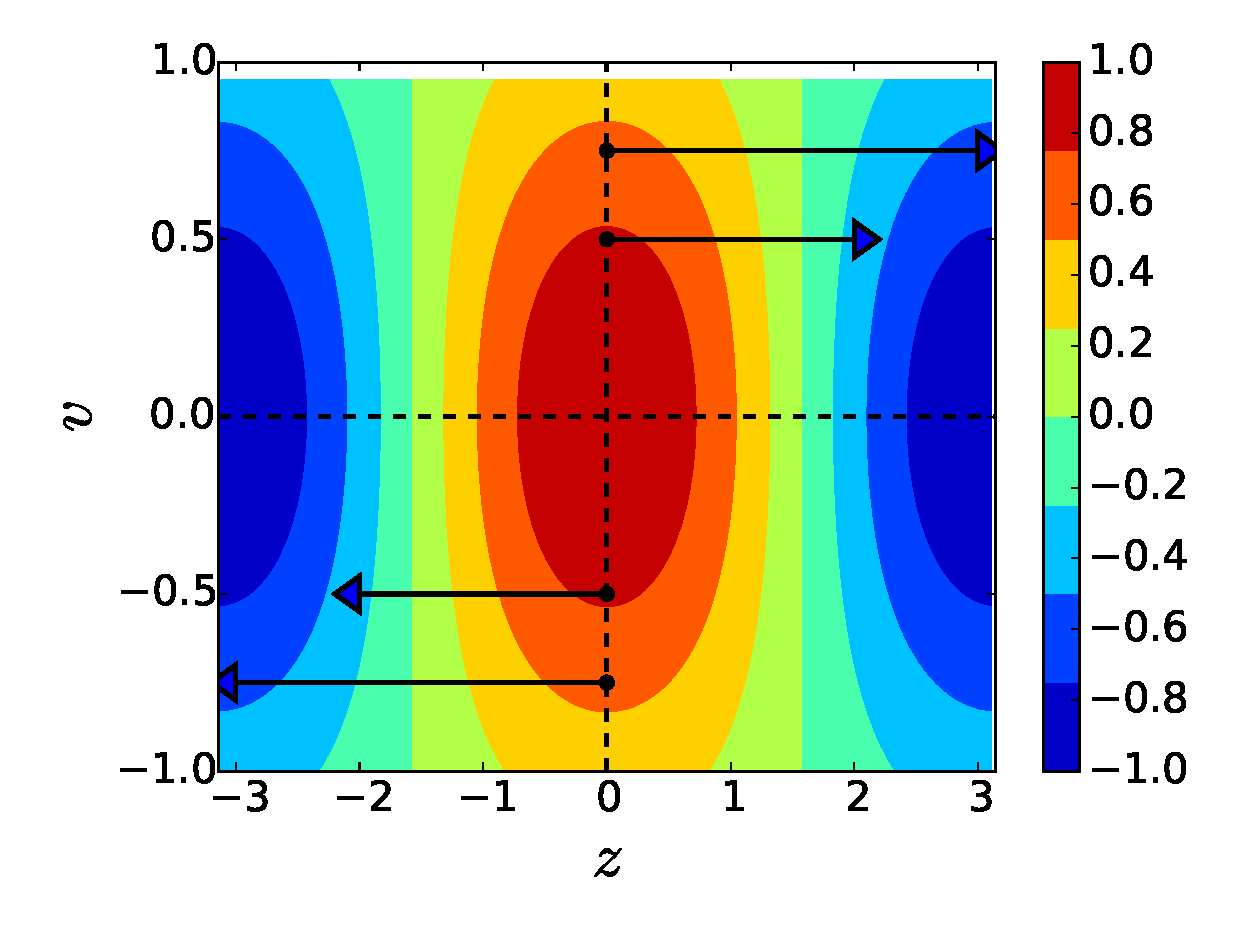
\includegraphics[width=7.4cm]{figs/intro/phmixt0.eps}
        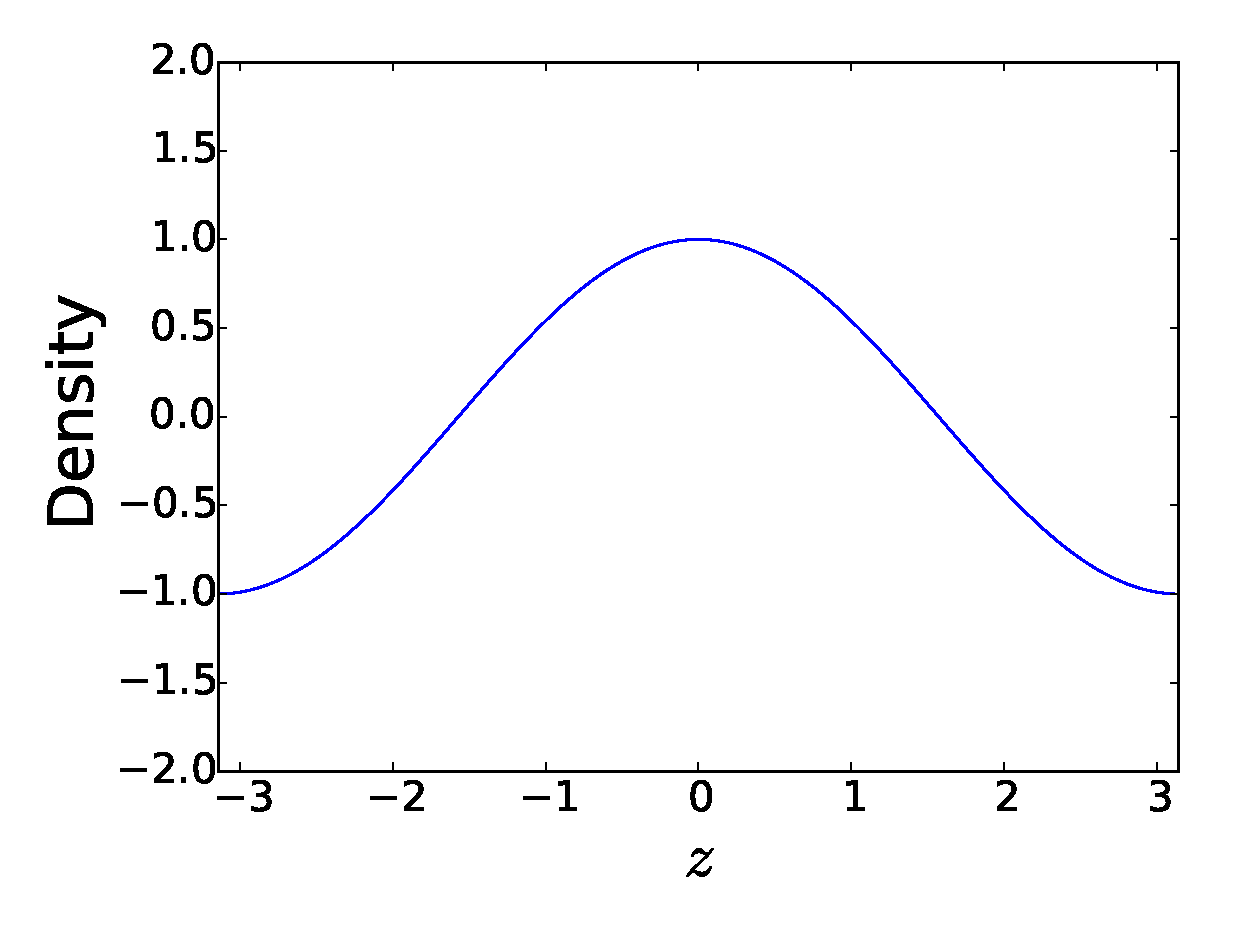
\includegraphics[width=7.4cm]{figs/intro/denst0.eps}
        \caption{The initial perturbed distribution function (left), and the corresponding density
        perturbation (right). }
        \label{intro:fig:t0}
     \end{center}
     \end{figure}

     \begin{figure}
     \begin{center}
        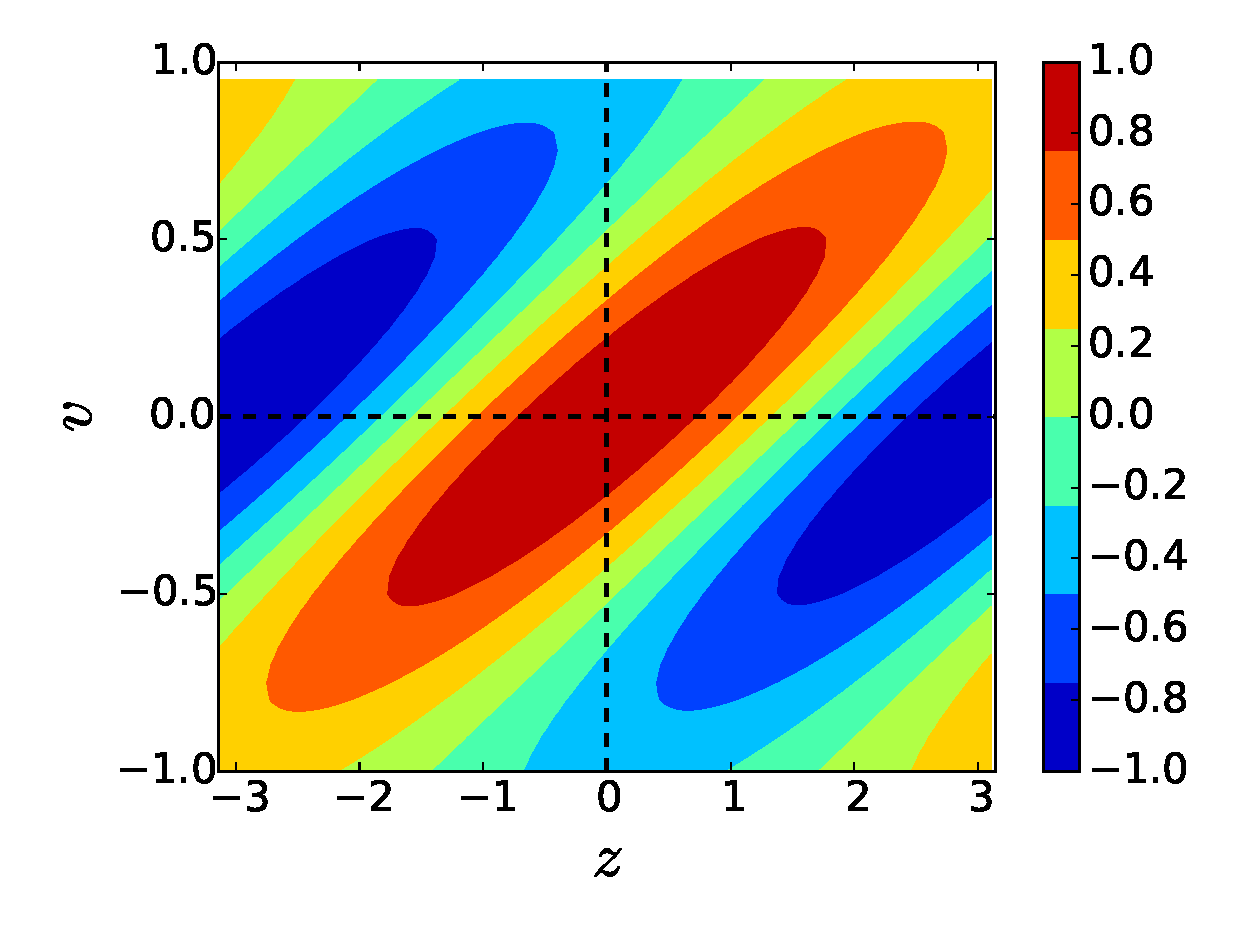
\includegraphics[width=7.4cm]{figs/intro/phmixt4.eps}
        \includegraphics[width=7.4cm]{figs/intro/denst4.eps}
        \caption{The perturbed distribution function (left), and the corresponding density
        perturbation (right) at time $t$.}
        \label{intro:fig:tt}
     \end{center}
     \end{figure}

     For a simple illustration of phase mixing, consider a
     homogeneous 1D plasma in equilibrium, with a perturbed ion distribution function
     $\delta f$: 
     \beq
        \delta f(z, v, t=0) = \cos(k z) F_0(v). \label{intro:eq:df:0}
     \eeq
     Here, the perturbation is assumed to be a cosine in the spatial direction $z$, and
     Maxwellian in velocity space, $F_0(v) = \exp\lt(-v^2/\vth^2\rt)/\sqrt{\pi}\vth$, where
     $\vth=\sqrt{2T/m}$ is the thermal velocity of the ions, $T$ is the ion temperature,
     and $m$ is the ion mass.
     This perturbed distribution function corresponds to a density perturbation $\delta n$: 
     \beq
        \delta n (z, t=0)  = \cos(k z), \label{intro:eq:dn:0}
     \eeq
     where $\delta n = \int dv\, \delta f$. The initial condition given by
     \eqsdash{intro:eq:df:0}{intro:eq:dn:0} is plotted in
     \figref{intro:fig:t0}.
     Ignoring electromagnetic effects, as time evolves, ions with different
     velocities move to different locations in space, generating structure in the
     perturbed distribution function with respect to $v$ at a
     constant $z$:
     \beq
        \delta f (z, v, t) = \cos(k z - k v t) F_0(v). \label{intro:eq:df:t}
     \eeq
     Since density is the integral of the distribution
     function over velocity ($\delta n = \int dv\, \delta f$), as the distribution function becomes more and more striated, the
     density diminishes: 
     \beq
        \delta n (z, t) = \cos(k z) \exp\lt(-k^2 \vth^2 t^2/4\rt). \label{intro:eq:dn:t}
     \eeq
     The perturbed distribution function and the perturbed density at time $t$ are plotted
     in \figref{intro:fig:tt}.
     This transfer of structure from real to velocity space, resulting in damping of low
     order velocity moments
     is known as phase mixing\footnote{There is another, nonlinear, phase mixing process
     \cite{tatsuno09}
     which plays an important role in the turbulence of weakly collisionless plasmas at scales
     comparable to the ion Larmor radius. 
      However, in
     this thesis we only consider turbulence at scales larger than the ion Larmor radius, and ignore
     this process. As a result, the linear phase mixing discussed here is the only phase mixing process in
     our models.}.

     In the collisionless limit, phase mixing is a reversible process. 
     The distribution function does not ``forget" the original perturbation that gets
     damped, and in theory, can return the system to its original state. The most famous
     example of such reversibility is the plasma echo \cite{gould67, malmberg68,
     malmberg68b, su68}. In these experiments, a perturbation of the electric potential is
     excited, which Landau damps away; later, another perturbation of the electric
     potential is excited, which also damps away; subsequently, a non-zero electric
     potential perturbation (the echo) is observed to appear in the
     plasma. The two original electric pulses couple nonlinearly to generate this echo.

     \begin{figure}
     \begin{center}
        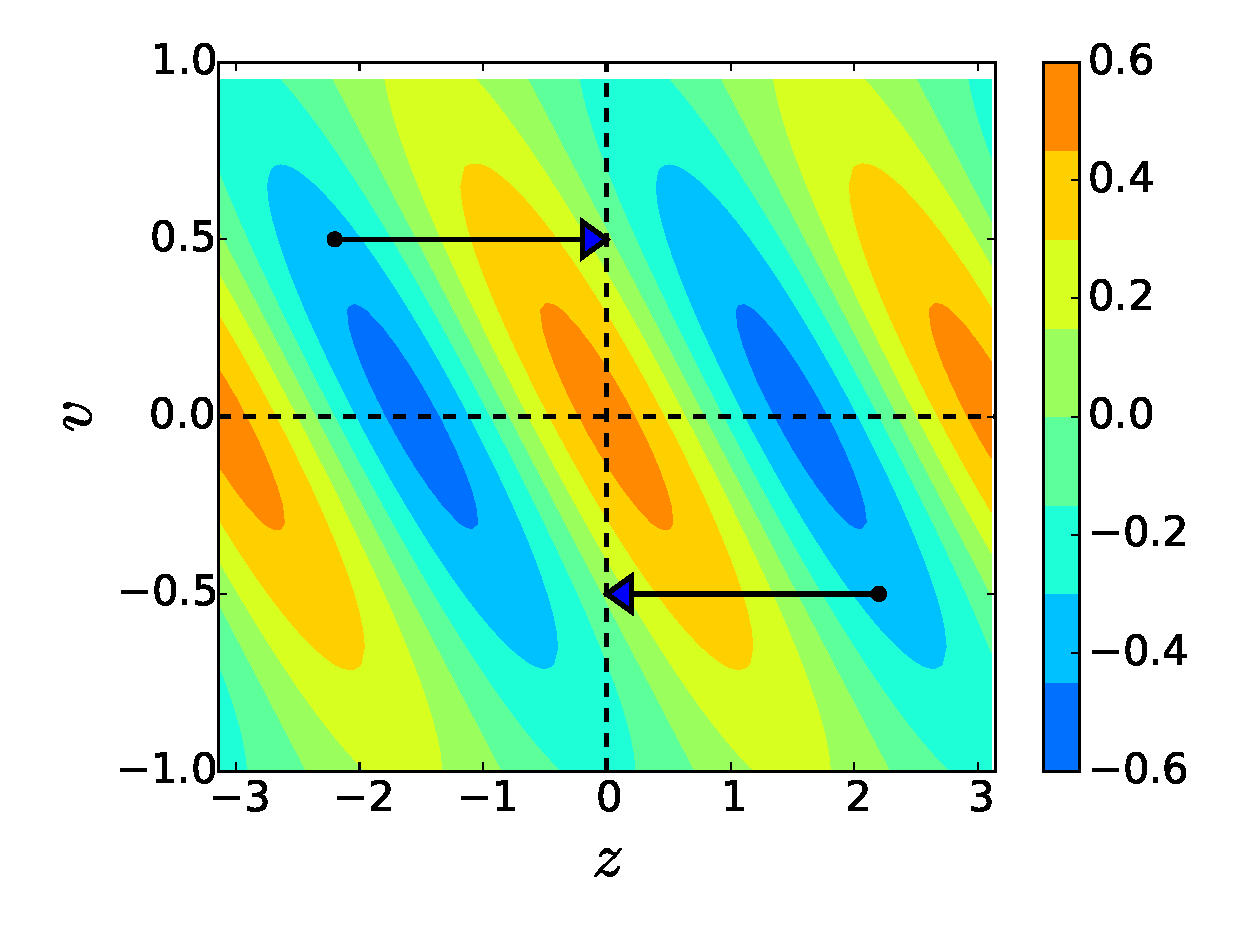
\includegraphics[width=7.4cm]{figs/intro/phmix_echot4.eps}
        \includegraphics[width=7.4cm]{figs/intro/denstecho4.eps}
        \caption{The perturbed distribution function (left), and the density perturbation
        (right), for a mode that is nonlinearly generated by the mode in
        \figref{intro:fig:tt}. It is assumed that this new mode has a wavenumber
        $p$, such that $\sgn(p) = -\sgn(k)$.} 
        \label{intro:fig:echo:t0}
     \end{center}
     \end{figure}

     \begin{figure}
     \begin{center}
        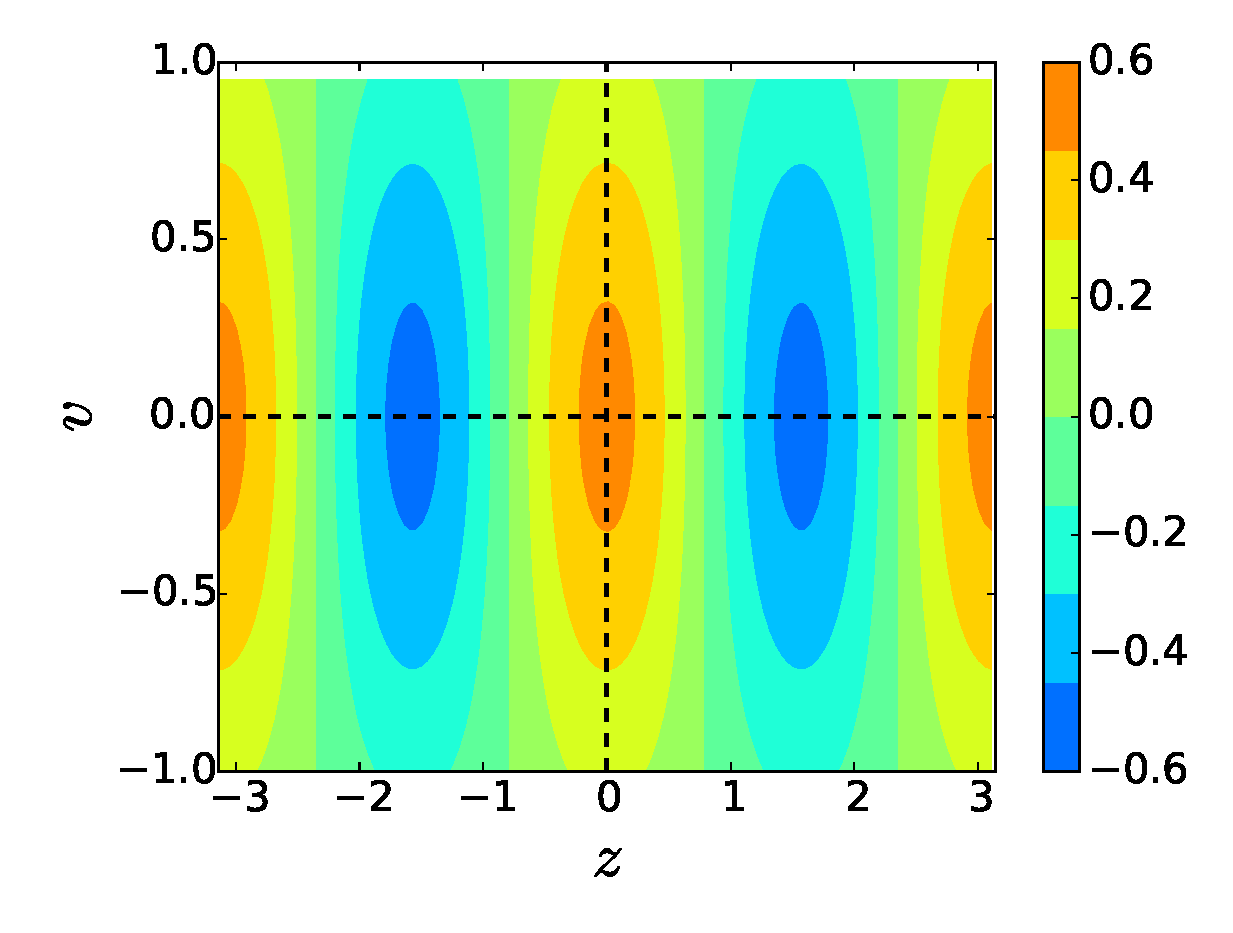
\includegraphics[width=7.4cm]{figs/intro/phmix_echot8.eps}
        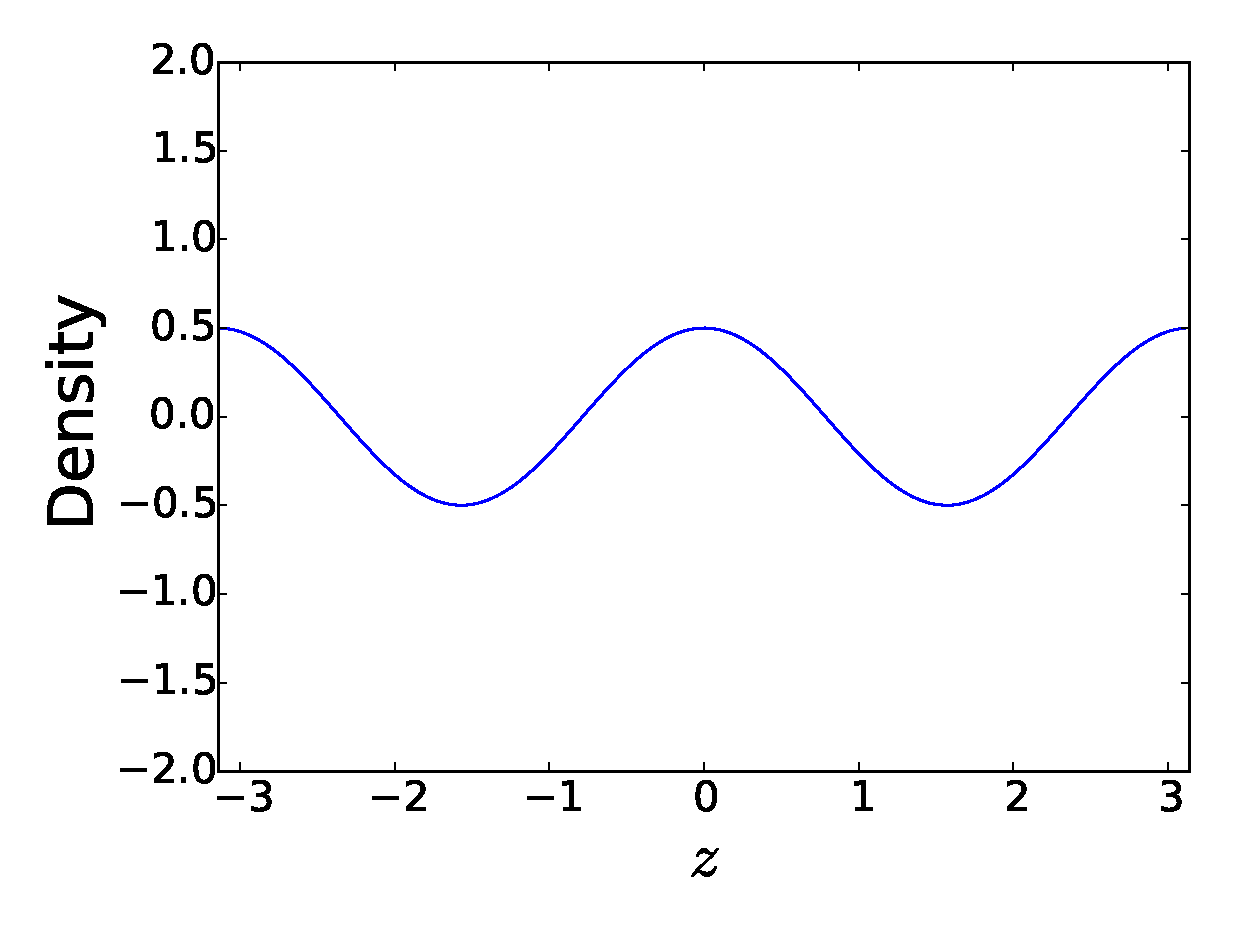
\includegraphics[width=7.4cm]{figs/intro/denstecho8.eps}
        \caption{The perturbed distribution function (left), and the density perturbation
        (right), for the mode shown in \figref{intro:fig:echo:t0}, at a later time
        $t \lt(1-k/p\rt)$.}
        \label{intro:fig:echo:tt}
     \end{center}
     \end{figure}
     
     The cartoon for phase mixing discussed above (see
     \figsand{intro:fig:t0}{intro:fig:tt}) can
     be extended to include the echo as follows.
     Imagine that the perturbation shown in \figref{intro:fig:tt} nonlinearly couples with
     another perturbation to generate
     a mode which has an oppositely signed wavenumber $p$:
     \beq
        \delta f_{\text{echo}} (z, v, t) = A \cos(p z - k v t) F_0(v),
     \eeq
     where $A$ is the amplitude of this new perturbation. This mode corresponds to a density
     perturbation given by
     \beq
        \delta n_{\text{echo}} (z, v, t) = A \cos(p z) \exp\lt(-k^2 t^2/4\rt).
        \label{intro:echo:eq:n0}
     \eeq
     The perturbed distribution function, and the density perturbation for this mode are
     plotted in \figref{intro:fig:echo:t0}. Observe that due to the change in sign of the
     wavenumber, the phase space contours of the perturbed distribution function are now tilted in the opposite way.
     At a later time $t+t'$, this perturbed distribution function evolves into
     \beq
        \delta f_{\text{echo}} (z, v, t+t') = A \cos(p z - p v t' - k v t) F_0(v).
     \eeq
     Since $p$ and $k$ are oppositely signed, the corresponding density perturbation
     at this later time is larger than the one in \eqref{intro:echo:eq:n0}:
     \beq
        \delta n_{\text{echo}} (z, v, t+t') = A \cos(p z) \exp\lt(-(kt+ pt')^2/4\rt).
     \eeq
     This perturbation is plotted in \figref{intro:fig:echo:tt} for time
     $t+t'=t\lt(1-k/p\rt)$. 
     %The generation of modes like the one shown in
     %\figref{intro:fig:echo:t0} by nonlinear interaction gives the plasma echo.

     It is shown in \chapref{chap:phmixlin} that the echo is inherently a nonlinear phenomenon, and is
     not observed for an isolated Fourier mode. In Chapters \ref{chap:pp0} and
     \ref{chap:phmixnl} nonlinear models are considered, where different Fourier modes are
     coupled to each other. Nonlinearly, the plasma echo may be observed.
     The necessary conditions required for an echo are discussed in detail within these chapters.
     

     \section{Turbulence}
     \label{intro:sec:turb}

    
    \begin{figure}
    \begin{center}
        \includegraphics[width=14.8cm]{figs/intro/turbcartoon.png}
        \caption{A cartoon picture of turbulence.}
        \label{intro:fig:turbcartoon}
    \end{center}
    \end{figure}
    Turbulence is ubiquitous, yet a precise definition of turbulence does not exist. 
	A simple picture of
	a turbulent system is depicted in \figref{intro:fig:turbcartoon}: energy is injected
	into the system at some large scale, which then cascades down to smaller and smaller
	scales. Eventually a dissipative process
	like viscosity takes over and dissipates the injected energy\footnote{\textit{Big whorls have
    little whorls that feed on their velocity, and little whorls have lesser whorls and so
    on to viscosity.}---Lewis F. Richardson}. The driving scale and
	the dissipative scale need to be far removed from each other for the system to exhibit
	turbulence. For this to be true the ratio of the driving length scale to the
	dissipation length scale, also known as the Reynolds number, is required to be large---a
    basic requirement for turbulence.

    For our purposes we broadly classify models of turbulence into two categories---fluid
    models and kinetic models. Fluid models describe systems where the mean
    free path for collisions is smaller than any length scale of interest, \ie,
    collisions are frequent. Whereas, kinetic models are applicable to systems where the
    mean free path is comparable to, or larger than the system size, \ie, collisions are
    rare. Henceforth, we use the terms ``fluid/kinetic model of
    turbulence", and ``fluid/kinetic turbulence" interchangeably.
    
    \subsection{Fluid turbulence}
    \label{intro:sec:turb:fluid}
    One of the
    first theories describing turbulence in neutral fluids was by Kolmogorov \cite{kolmogorov41},
    in which he predicts the famous $k^{-5/3}$ power law spectrum for homogeneous
    isotropic turbulence. In order to derive this spectrum, he
    made some key assumptions that have come to underlie turbulence theory: 
    \begin{inparaenum}[(i)]
        \item  statistical properties of turbulence, such as the energy spectrum, are universal at scales in between the injection and dissipation scale;
        \item the energy transfer from large to small scales happens locally in wavenumber
        space;
        \item no energy is lost at the intermediate scales, in other words, the flux of
        energy through each scale is independent of the scale.
    \end{inparaenum}

    Under these assumptions the energy density spectrum can be derived as follows: let
    $u_\lambda$ be a velocity fluctuation at the length-scale $\lambda$. The (constant) flux of energy
    $\epsilon$ through the scale $\lambda$ is then given by,
    \beq
        \frac{u_\lambda^2}{\tau_\lambda}\sim \epsilon,
    \eeq
    where $\tau_\lambda^{-1}$ is the energy cascade rate at scale $\lambda$. Since
    the energy transfer to smaller scales is local, the cascade rate must be a function
    of quantities that depend on $\lambda$. Since $u_\lambda$ and $\lambda$ are the only
    physical quantities available, the cascade rate can be estimated as,
    \beq
        \tau_\lambda \sim \frac{\lambda}{u_\lambda}.
    \eeq
    Therefore, 
    \beq
        u_\lambda^2 \sim (\epsilon \lambda)^{2/3}. \label{intro:eq:ulambda}
    \eeq
    Hence, the energy spectrum is a power law $k^{-\alpha}$. For $u_\lambda^2 \propto
    \lambda^g$, the spectral exponent $\alpha$ is calculated as $\alpha = g + 1$
    \cite{monin75}. Therefore, from \eqref{intro:eq:ulambda}, the energy spectrum for 
    turbulence in the fluid limit is $k^{-5/3}$. 
    
	The power law spectrum is characteristic of broadband fluctuations, which may
	be thought of as a signature of turbulent systems.

    \subsection{Kinetic turbulence}
    \label{intro:sec:turb:kinetic}

    \begin{figure}
    \begin{center}
        \includegraphics[width=7.4cm]{figs/intro/collisions_gas.png}
        \includegraphics[width=7.4cm]{figs/intro/collisions_plasma.png}
        \caption{Collisions in neutral fluids (left) result in sharp changes in velocity.
        Whereas, a particle (ion or electron) in a plasma undergoes many small-angle collisions
        (right). Therefore, collisions can be modeled as a diffusive operator in the
        velocity co-ordinate.}
        \label{intro:fig:collisions}
    \end{center}
    \end{figure}
    In this section, we shall move away from the discussion about neutral fluid turbulence, and discuss the
    general properties of turbulence in weakly collisional plasmas.
    In addition to the fluid-like turbulent cascade in real space, weakly collisional
    systems also allow for   
    transfer of energy to small velocity space scales by phase mixing. This makes the nature
    of dissipation for such systems a contentious issue \cite{parashar13}.
	Even though phase mixing damps
    perturbations in the plasma, the process is reversible in the
	collisionless limit, \ie, it does not generate 
	entropy. Therefore, phase mixing is not dissipative in the true sense. Irreversible heating for these systems is only possible through collisions
	\cite{schekochihin08, tome}. Collisions in plasmas are of a different character than
    the ones in neutral fluids (see \figref{intro:fig:collisions}). Unlike neutral fluids,
    particles (ions or electrons) in a plasma undergo numerous long-range collisions, which
    individually do not
    alter the velocity of the particle by much. 
	Therefore, collisions can be modeled as a diffusive operator in velocity space: $\sim \nu \,
	\partial_v^2$ \cite{howes06, tome}, where $\nu$ is the frequency with which a particle velocity is changed by
    $\pi/2$ radians. For systems with vanishingly
	small $\nu$, energy has to be transferred to small scales in velocity space, before it
    can dissipate via collisions. As a result, in the weakly collisional limit, the cascade of energy
    occurs in the phase space (real and velocity space) \cite{schekochihin08, tome,
    tatsuno09}---the spatial cascade is the usual fluid-like nonlinear refinement of
    scales, whereas the cascade in velocity space is due to phase mixing.
    
    The systems studied in this thesis are assumed to be weakly collisional, and allow for 
    the above mentioned phase space cascade. 

\section{Magnetized plasmas}

    In addition to assuming that the plasma is weakly collisional, it
    is also assumed to be strongly magnetized. A strongly magnetized plasma is threaded by
    a mean magnetic field such that the ion Larmor radius is much smaller than the system
    size. Additionally, it is assumed that
    the magnitude of the background magnetic field is much larger than the turbulent electromagnetic fluctuations. For
    magnetic confinement fusion devices, this is a given, as a guide field is necessary for
    confinement of the burning plasma. For space and astrophysical plasmas, the large scale
    magnetic fluctuations behave as a background magnetic field for the small scale
    turbulence (Kraichnan hypothesis \cite{kraichnan65}). 

    The background magnetic field makes these systems very anisotropic \cite{goldreich95,
    goldreich97}---the
    perpendicular length scales ($\lambda$) are much smaller than the parallel length
    scales ($l$). For such anisotropic systems, the Kolmogorov derivation for the energy spectrum is no longer
    possible, since the timescale at a given scale cannot be determined uniquely. There
    is a perpendicular, nonlinear timescale $\lambda/u_\lambda$, and a parallel,
    linear timescale associated with the Alfv\'{e}n waves $l/v_A$,
    where $v_A$ is the Alfv\'{e}n velocity. In the magnetohydrodynamic limit, Goldreich and Sridhar \cite{goldreich95,
    goldreich97} proposed a way forward by assuming that the turbulence, at sufficiently
    small scales, arranges itself in such a way that the linear and nonlinear
    timescales are comparable to each other \cite{galtier00, schekochihin12}. This assumption, taken scale by scale is
    known as \textit{critical balance}. One can then estimate the cascade time as
    \beq
        \tau_\lambda \sim \frac{\lambda}{u_\lambda} \sim \frac{l}{v_A},
    \eeq
    which once again gives,
    \beq
        u_\lambda \sim (\epsilon \lambda)^{1/3}.
    \eeq
    This again corresponds to a $k_\perp^{-5/3}$ spectrum, but now the spectrum is in the
    perpendicular direction, as opposed to the isotropic spectrum derived earlier for neutral
    fluids.
    The critical balance
    assumption also relates the parallel and perpendicular length scales:
    \beq
        l \sim l_0^{1/3}\lambda^{2/3}, \label{intro:eq:critanis:l}
    \eeq
    where $l_0 = v_A^3/\epsilon$; $l_0$ is the parallel length scale where the velocity
    fluctuation is comparable to the Alfv\'{e}n velocity, and can be thought of as a
    natural outer scale. Therefore, the velocity fluctuation scaling with respect to $l$
    is given by 
    \beq
        u_\lambda \sim \lt(\frac{\epsilon^{1/3}}{l_0^{1/6}}\rt) l^{1/2}.
    \eeq
    This corresponds to a parallel spectrum of
    $\kpar^{-2}$. The relationship given by \eqref{intro:eq:critanis:l} between the parallel and
    perpendicular length scales looks like $\kpar~\sim~k_\perp^{2/3}$ in terms of the
    wavenumbers, \ie, as the cascade moves forward to smaller spatial scales, it gets
    increasingly anisotropic.

    In addition to the spatial scale separation, the background magnetic field also
    separates timescales. The cyclotron motion may be assumed to be much faster than any
    timescale of interest in
    the system---this allows for reduced descriptions of kinetic plasmas, which are
    discussed further in \secref{intro:sec:krmhd} and \apref{app:eq}.

\section{Phase mixing in turbulent magnetized plasmas: Questions}
    
    In \secsand{intro:sec:phmix}{intro:sec:turb} we discussed how phase mixing
    and turbulent cascade dictate the turbulent characteristics of a plasma individually. It is
    however unclear, as to
    what happens to phase mixing in a nonlinear turbulent system. Understanding how phase
    mixing works in presence of turbulence is an important problem in kinetic plasma
    turbulence.

     \begin{figure}
     \begin{center}
        \includegraphics[width=7.4cm]{figs/intro/Armstrong_dens.jpg}
        \includegraphics[width=7.4cm]{figs/intro/solarwind_dens.jpg}
        \caption{Density fluctuation spectra in the interstellar medium (left, taken from
        \cite{armstrong95}) and the solar wind (right, taken from \cite{marsch90}). These power law
        spectra span multiple decades, even at scales where these fluctuations are
        expected to be strongly damped.}
        \label{intro:fig:dnespec}
     \end{center}
     \end{figure}

    A simple way to incorporate phase mixing in a model for a turbulent plasma 
    would be to introduce it as
    a sink of energy to small velocity
    scales, at each spatial scale, in essence superimposing phase mixing
    on to the turbulent cascade \cite{quataert98, quataert99, howes08jgr}. For the cascade of a macroscopic quantity like
    density fluctuations, this would show up as a scale-by-scale dissipative term, where the rate of
    dissipation is proportional to the parallel wavenumber. 
    Such dissipation would violate the constant-flux-through-scales assumption of
    Kolmogorov. Extraction of energy at each scale at a rate proportional to
    the wavenumber
    would imply that the energy spectrum 
    should be an exponential decay instead of a power law.
    However, power law energy spectra are commonly observed in weakly collisional turbulent
    magnetized plasmas.
    A striking example is that of compressive
    fluctuations in astrophysical systems. Electron density
    fluctuations in the interstellar medium extend over twelve decades of scales, 
    famously known as ``the Great Power Law in the Sky" \cite{armstrong81, armstrong95,
    lazio04}. In the solar wind, these
    fluctuations are observed for roughly three decades \cite{lovelace70, woo79, celnikier83,
    celnikier87, coles89, marsch90, coles91, bershadskii04, hnat05, kellogg05,
	alexandrova08} (see \figref{intro:fig:dnespec}). These observations are at scales
    where the plasma is weakly collisional. Linear theory predicts that compressive
    fluctuations should be strongly damped in the weakly collisional limit \cite{barnes66}, which makes
    these observed power law spectra surprising.
    This suggests that when the system is nonlinear, the linear predictions need to be
    modified.
    A possible explanation for such power law spectra, though not specifically for these
    plasmas, was given recently by Plunk \etal\
    \cite{plunk13, plunk14}, where they argue that phase mixing is suppressed due to
    what is in essence, an ``impedance mismatch" with the nonlinear turbulent frequency.
	However, in
    their study, they do not include the nonlinear cascade. Instead, they consider a
    single Fourier mode, and add a random source term as a stand-in for
    turbulence---this approach is quite different from the one we adopt here.

    In this thesis, the interplay between the nonlinear cascade and phase mixing is
    studied.
    This is done by considering nonlinear models which incorporate both these effects\footnote{This is different from what is generally referred to as nonlinear
    Landau damping (see \cite{mouhot11} and references therein for a detailed analysis of
	this problem from a mathematician's perspective) in the literature. The question there
	is what happens to the validity of Landau's results
    if the perturbations have finite amplitudes. In our work, all perturbations are
    assumed small compared to the equilibrium.}.
%     In chapter \ref{chap:phmixlin}, we analytically derive the behavior of a
%     driven-damped system in absence of
%    turbulent cascade. In chapters \ref{chap:pp0} and \ref{chap:phmixnl}, we consider 
%    simple models of kinetic passive scalar turbulence, where we discuss the fate of phase
%    mixing in the presence of turbulent cascade. In
%    \chapref{chap:slowmodes}, we present results from direct numerical simulations of
%    compressive fluctuations in the solar wind, and describe a possible mechanism that
%    would explain the observed power law spectra for density and field strength
%    fluctuations at kinetic scales (\figref{intro:fig:dnespec}). The numerical tool developed for this work
%    is described in \chapref{chap:gandalf}.
%    
%    It is important to understand what happens to phase
%    mixing in presence of turbulence in order to address this discrepancy.
%    At this point it is important to mention that 
%    ``Landau fluid" models\cite{hammett90, hammett92, hedrick92, dorland93, beer96,
%    snyder97, snyder01, snyder01gf, passot04, ramos05, goswami05, passot06, passot07,
%    passot12}, though more sophisticated in nature, use the same basic
%    principle of extracting energy from higher velocity moments at the linear damping
%    rate. These models have shown tremendous success in reproducing experimental results
%    for fusion plasmas, and seem to be generally used in scenarios where phase mixing
%    remains essentially unaltered due to turbulence.
%
%
    The first nonlinear model allows for a turbulent cascade in the direction
    perpendicular to the guide field, but does not allow for a transfer of energy to small
    spatial scales parallel to the background field. In this scenario, when the turbulent
    cascade rate is comparable to or larger than the phase mixing rate, energy gets swept up
    to small spatial scales before it can phase mix. As a result a fluid-like turbulent
    cascade, \ie\, a power law spectrum is observed. In the other, more interesting model, where the turbulent cascade
    proceeds in both perpendicular and parallel directions, 
    a turbulent analog
    of the plasma echo is observed, which unravels the velocity space structure generated by
    phase mixing. This
    \textit{stochastic plasma echo} suppresses phase mixing, which again results in a fluid-like
    turbulent cascade at scales where, in the linear limit, perturbations would be
    strongly damped due to phase mixing. Hence, regardless of whether or not there is a
    parallel cascade, power law energy spectra are observed for
    turbulent fluctuations at these ``kinetic" scales.
    
    \section{Kinetic Reduced MHD}
    \label{intro:sec:krmhd}
    \subsection{Basic framework}
    
    The basic mathematical framework used in this work is
    known as Kinetic Reduced MagnetoHydroDynamics (KRMHD). KRMHD is the
    long wavelength limit of gyrokinetics \cite{rutherford68, taylor68, catto78, antonsen80,
    catto81, frieman82, dubin83, lee83, lee87, hahm88, howes06, tome}. It is derived in
    thorough detail in Schekochihin \etal\ \cite{tome}, by expanding ``$\delta f$ gyrokinetics"  in small $k_\perp \rho_i$ ($k_\perp$ is the perpendicular wavenumber,
    $\rho_i$ is the ion Larmor radius). In this limit, the Alfv\'{e}nic component of
    the cascade
    decouples from the compressive fluctuations. The dynamics of the system are completely
    determined by the Alfv\'{e}nic fluctuations, which evolve according to reduced MHD
    \cite{kadomtsev74, strauss76}. The compressive
    fluctuations, on the other hand, are described by a kinetic equation for a passive
    scalar that is nonlinearly advected by the background Alfv\'{e}nic turbulence. These
    equations provide an efficient framework within which one may study the turbulent cascade
    of density and field strength fluctuations in weakly collisional turbulent magnetized
    plasmas like the solar wind. 
    
    The passive nature of compressive fluctuations in this
    model neatly ties in with a popular approach used to study turbulent cascade in fluid
    systems, namely that of passive scalar turbulence \cite{obukhov49, corrsin51, batchelor59,
    kraichnan68, kraichnan74, kraichnan94,
    monin75, aref84, chaiken87, ottino89, zeldovich88, ott88, ott89, antonsen91, ramashankar91,
    solomon93, sreenivasan91,
    vanatta91, pierrehumbert94, antonsen95, frisch95, sreenivasan96, boratav97, lesieur97, shraiman00,
    warhaft00}. This gives us the opportunity to study the general problem of
    \textit{kinetic} passive
    scalar turbulence, while having a physically relevant system to compare with.
    General results regarding kinetic passive scalar turbulence are presented in Chapters
    \ref{chap:phmixlin}, \ref{chap:pp0} and \ref{chap:phmixnl}, by considering simplified
    versions of KRMHD. The full KRMHD equations are
    numerically solved in \chapref{chap:slowmodes}.

    The derivation of KRMHD given in Schekochihin \etal\ \cite{tome} is extremely detailed, and we
    do not attempt to better it in this thesis. Instead, we give an outline of the
    derivation of KRMHD in \apref{app:eq}, and give a summary of the final equations here.
    
    The KRMHD model assumes a homogeneous equilibrium, with a Maxwellian as the background
    distribution function. A perturbation of this equilibrium is evolved in time. 
    The Alfv\'{e}n cascade is described by reduced MHD,
    which in its simplest form is written in terms of Elsasser variables \cite{elsasser50}:
    \beq
    \pd{\nabla_\perp^2 \xi^\pm}{t} \mp v_A \pd{\nabla_\perp^2 \xi^\pm}{z} = - \frac{1}{2} \left[
    \{\xi^+, \nabla_\perp^2 \xi^- \} + \{\xi^-, \nabla_\perp^2 \xi^+ \} \mp \nabla_\perp^2
    \{\xi^+, \xi^-
    \} \right], \label{intro:krmhd:els} 
    \eeq
    where the background magnetic field $\mb{B}_0 = B_0\hat{\mb{z}}$ is in the
    $\hat{\mb{z}}$ direction, $\hat{\mb{x}}$ and $\hat{\mb{y}}$ are the transverse directions,
    $\xi^\pm = \Phi \pm \Psi$, $v_A = B_0/\sqrt{4 \pi m_i n_{0i}}$ is the Alfv\'{e}n
    velocity, and $\Phi$ and $\Psi$ are stream and flux functions
    respectively, which are related to the electrostatic potential ($\phi$) and the magnetic vector
    potential ($\Apar$) by:
    \beq
        \Phi = \frac{c}{B_0}\phi, \quad \Psi = - \frac{\Apar}{\sqrt{4 \pi m_in_{0i}}}
        \label{intro:eq:PhiPsi},
    \eeq
    where $c$ is speed of light,
    $m_i$ is the ion mass, and $n_{0i}$ is the background ion density.
    The braces denote the Poisson bracket:
    \beq
        \lt\{P,Q\rt\} = \pd{P}{x}\pd{Q}{y} - \pd{P}{y} \pd{Q}{x}.
    \eeq

    The left hand side of \eqref{intro:krmhd:els} describes Alfv\'{e}n wave packets,
    traveling up or down the field line. The nonlinear interaction between these wave
    packets is captured by
    the right hand side. Observe that only counter-propagating Alfv\'{e}n waves interact
    nonlinearly; these counter-propagating Alfv\'{e}n waves give rise to the turbulent cascade by
    transferring energy to smaller spatial scales.

    The compressive fluctuations are described in terms of two Elsasser-like variables
    $g^+$ and $g^-$:
    \beq
    \od{g^\pm}{t} + \vpar \nabla_\parallel g^\pm  = \frac{\vpar F_0(\vpar)}{\Lambda^\pm}
    \hat{\mb{b}}\cdot\nabla \int d \vpar g^\pm, \label{intro:krmhd:gpm}
    \eeq
    where $F_0(\vpar)=\exp(-\vpar^2/\vth^2)/\sqrt{\pi} \vth$ is a one-dimensional
    Maxwellian ($\vth=\sqrt{2T_i/m_i}$ is the thermal velocity of ions, $T_i$ is the ion
    temperature, $m_i$ is the ion mass), and
    \beq
        \Lambda^\pm = -\frac{\tau}{Z} + \frac{1}{\beta_i} \pm \sqrt{\lt(1 +
        \frac{\tau}{Z}\rt)^2 + \frac{1}{\beta_i^2}}, \label{intro:krmhd:Lambda}
    \eeq
    where $\tau$ is the ion to electron temperature ratio, $Z$ is the ion charge in units
    of the electron charge, and $\beta_i = 8\pi n_{0i} T_i/B_0^2$ is the ion plasma beta.
    We observe from \eqref{intro:krmhd:Lambda}, that the range of $\Lambda^\pm$ is
    restricted to: $\Lambda^+ > 1$, and $\Lambda^- < 0$. The derivatives $d/dt$ 
    and $\nabla_\parallel$ in \eqref{intro:krmhd:gpm} are convective derivatives:
    \beq
        \od{}{t} = \pd{}{t} + \lt\{\Phi,\ldots\rt\}, \quad \nabla_\parallel =
        \pd{}{z} + \frac{1}{v_A}\lt\{\Psi,\ldots\rt\}.\label{intro:krmhd:convder}
    \eeq
    The relationship between
    the perturbed ion distribution function and $g^\pm$ is given in \apref{app:eq} (see
    \eqsand{eqs:eq:gnBdef}{eqs:krmhd:gpmdef}).
%These are in fact described 
%by two equations evolving two decoupled 
%functions $g^+$ and $g^-$, which are certain linear combinations 
%of the zeroth and second moments of the perturbed ion distribution 
%function with respect to the velocity perpendicular to the 
%mean magnetic field (taken to be in the $z$ direction). 
%These equations are derived in \cite[][\S 6.2.1]{tome} 
%and are of the form \exref{phmixlin:eq:g} with 
%\beq
%\alpha^\pm =-\lt[-\frac{T_i}{ZT_e} + \frac{1}{\beta_i}\pm A\rt]^{-1}, \quad
%A = \sqrt{\lt(1+\frac{T_i}{ZT_e}\rt)^2 + \frac{1}{\beta_i^2}} 
%\eeq
%for $g^\pm$, respectively (here $\beta_i=8\pi n_iT_i/B^2$ is the ion beta). 
%The physical fields, the density and magnetic-field-strength perturbations, are related 
%to $g^\pm$ by 
%\begin{align}
%\frac{\delta n}{n} &= \frac{1}{2A}\int\rmd v\lt[\lt(1 + \frac{T_i}{ZT_e} + \frac{1}{\beta_i} + A\rt)g^-
%- \frac{T_i}{ZT_e}\frac{2}{\beta_i}\,g^+\rt],\\
%\frac{\delta B}{B} &= \frac{1}{2A}\int\rmd v\lt[\lt(1 + \frac{T_i}{ZT_e} + \frac{1}{\beta_i} + A\rt)g^+
%- \lt(1+\frac{ZT_e}{T_i}\rt)g^-\rt].
%\end{align}
%While these expressions are perhaps not very physically transparent, it may aid 
%intuition to note that ${\delta n}/{n} \approx \int\rmd v g^-$ and 
%${\delta B}/{B} \approx \int\rmd v g^+$ either in the limit of 
%high $\beta_i$ and hot ions ($T_i\gg T_e$) or in the limit of 
%low $\beta_i$ and cold ions ($T_i\ll T_e$). At low $\beta_i$, the $g^-$ equation 
%describes ion-acoustic waves ($\alpha^-\approx ZT_e/T_i$; see above). 
%At high $\beta_i$, the $g^+$ equation describes a kinetic version of the MHD slow mode, 
%subject to a version of Landau damping due to \cite{barnes66}; 
%in this case, $\alpha^+\approx -1 + 1/\beta_i$. 
%
    \Eqsand{intro:krmhd:els}{intro:krmhd:gpm} together constitute the KRMHD model.

    \subsection{Conserved quantities}
    \label{intro:sec:krmhd:const}


    The energies in each of the Elsasser variables ($\xi^\pm, g^\pm$) are conserved
    independently in KRMHD:
    \beq
        W = W_{\text{AW}}^+ + W_{\text{AW}}^- + W_{\text{compr}}^+ + W_{\text{compr}}^-,
    \eeq
    where 
    \beq
        W_{\text{AW}}^\pm = \int d^3\mb{r} \frac{m_i n_{0i}}{2}
        \lt|\nabla_\perp\xi^\pm\rt|^2
    \eeq
    are energies of the right and left-going Alfv\'{e}nic fluctuations, and
    \beq
        W_{\text{compr}}^\pm = \int d\mb{r}\frac{n_{0i}T_{0i}}{2}\lt[\int d\vpar
        \frac{\lt(g^\pm\rt)^2}{F_0} - \frac{1}{\Lambda^\pm}\lt(\int d\vpar
        g^\pm\rt)^2\rt] \label{intro:eq:Wcomp}
    \eeq
    are energies of the $+$ and $-$ components of the compressive
    fluctuations\footnote{Both the terms in \eqref{intro:eq:Wcomp} are positive for
    the ``$-$" mode, since $\Lambda^- < 0$. For the ``$+$" mode, $W_{\text{compr}}^+$ can be
    shown to be positive using Cauchy-Schwarz inequality, and the condition $\Lambda^+>1$.}, as
    defined in the previous section, respectively; $W$ is the total free energy.


%\renewcommand{\thechapter}{3}
\chapter{Gandalf}
\label{chap:gandalf}

\section{Introduction}
    We have developed a new code called \Gand\ \footnote{The code solves for
    \textit{$g$-and-Alf}v\'{e}n waves, hence the name.} to solve the KRMHD
    \eqsand{intro:krmhd:els}{intro:krmhd:gpm}. \Gand\,
    is written in CUDA, a GPU computing platform and programming model invented by NVIDIA,
    and is an efficient numerical tool to study the long-wavelength asymptotic behavior
    of anisotropic magnetized plasmas.

\section{Equations}
    
     Instead of directly solving \eqref{intro:krmhd:gpm}, we first expand $g$ in
     \eqref{intro:krmhd:gpm} (superscripts will be suppressed whenever no confusion would
     result) in terms of its Hermite moments. Evolving
    the moments of $g$ instead of using a grid in velocity space makes the numerical
    scheme spectrally accurate in the $\vpar$ coordinate. 
    Expanding \eqref{intro:krmhd:gpm} in terms of Hermite polynomials also provides an
	elegant analytical framework to study phase mixing (see
	\chapref{chap:phmixlin} for details).
    The Hermite moments are defined as follows:
    \beq
    g(\vpar) = \sum_{m=0}^\infty \frac{H_m (\vpar/\vth) F_0 }{\sqrt{2^m m!}} g_m, \quad
    g_m = \int \rmd \vpar\, \frac{H_m(\vpar/\vth)}{\sqrt{2^m m!}}\, g(\vpar), 
    \eeq
    where $H_m$ is the Hermite polynomial of order $m$. \Eqref{intro:krmhd:gpm} then becomes a
    fluid-like hierarchy of equations:
    \begin{align}
        \label{gandalf:eq:g0}
        &\od{g_0}{t} + \vth \nabla_\parallel\frac{g_1}{\sqrt{2}}  = 0, \\
        \label{gandalf:eq:g1}
        &\od{g_1}{t} + \vth \nabla_\parallel\lt(g_2 + \frac{\lt(1-1/\Lambda\rt)}{\sqrt{2}}\,g_0\rt)
        = 0,\\
        &\od{g_m}{t} + \vth \nabla_\parallel\lt(\sqrt{\frac{m+1}{2}}\,g_{m+1} +
        \sqrt{\frac{m}{2}}\,g_{m-1}\rt) \nonumber \\
        &= C[g_m],  \quad m\ge2.
        \label{gandalf:eq:gmeq}
    \end{align}
    The first term on the right hand side of \eqref{intro:krmhd:gpm}, being proportional to 
    $H_1$, only appears in \eqref{gandalf:eq:g1}. The parallel
    streaming term couples each Hermite moment to the previous and the next moment\footnote{This is a result of the Hermite recurrence relation: $H_{m+1}(v) = 2 v
	H_m(v)- 2 m H_{m-1}(v)$.}. Dynamical coupling of different Hermite moments
    is the mathematical manifestation of linear phase mixing in Hermite space. 

    The right hand side of \eqref{gandalf:eq:gmeq} has a collision operator $C[g_m]$ that
    has been added to the kinetic \eqref{intro:krmhd:gpm}. Collisions are included in order to regularize the system at small velocity space scales. More
    importantly, they are also physically required to generate entropy and heat the 
    plasma---an exactly collisionless limit is unphysical.
    We choose a convenient collision operator, the Lenard--Bernstein 
    collision operator \cite{lenard58}, which in Hermite space looks like:
    \beq
        C[g_m] = - \nu m g_m,
    \eeq
    where $\nu$ is the collision frequency. The collision operator acts only on
    the second and higher Hermite moments, and hence, conserves particle number and
    momentum. This particular collision operator is also manifestly most effective for the highest
    moments retained, since $C[g_m] \propto m$.
    
    \Eqref{intro:krmhd:els} and
    \eqsdash{gandalf:eq:g0}{gandalf:eq:gmeq} are the equations that are
    implemented in \Gand.
    
\section{Normalization}

    We normalize the perpendicular spatial co-ordinates $x, y$ and the parallel spatial
    co-ordinate $z$, to independent arbitrary length scales $\rho$ and $L$, respectively
    (with the assumption $L \gg \rho$). By normalizing parallel and perpendicular
    co-ordinates independently, we can simulate highly anisotropic fluctuations with
    a numerical box that is roughly a cube. In addition, since the ratio $L/\rho$ is
    arbitrary, a single run simulates a whole range of problems with varying degrees of
    anisotropy.  
     Time is normalized to $L/v_A$. 
    The Elsasser fields $\xi^\pm$ are normalized to $\rho v_A$ (gradients of the Elsasser
    fields have units of velocity---see \eqref{intro:eq:PhiPsi}).  The Hermite moments $g_m$ of
	the perturbed
    distribution function $g$ are in arbitrary units. The Elsasser fields $\xi^\pm$, and
	the distribution function moments $g_m$
    are scaled up by a factor of $L/\rho$ so that all normalized terms have unity order of
    magnitude.
    
The normalized equations can then be written as, 
\begin{align}
    \pd{\nabla_\perp^2 \xi^\pm}{t} \mp \pd{\nabla_\perp^2 \xi^\pm}{z} & = - \frac{1}{2} \left[
    \{\xi^+, \nabla_\perp^2 \xi^- \} + \{\xi^-, \nabla_\perp^2 \xi^+ \} \mp \nabla_\perp^2
    \{\xi^+, \xi^-
    \} \right], \label{gandalf:eq:rmhd:norm}
\end{align}
\begin{align}
    \label{gandalf:eq:g0:norm}
    &\od{g_0}{t} + \sqrt{\beta_i} \nabla_\parallel\frac{g_1}{\sqrt{2}}  = 0,\\
    \label{gandalf:eq:g1:norm}
    &\od{g_1}{t} + \sqrt{\beta_i} \nabla_\parallel\lt(g_2 + \frac{1-1/\Lambda}{\sqrt{2}}\,g_0\rt)
    = 0,\\
    &\od{g_m}{t} + \sqrt{\beta_i} \nabla_\parallel\lt(\sqrt{\frac{m+1}{2}}\,g_{m+1} +
    \sqrt{\frac{m}{2}}\,g_{m-1}\rt) \nonumber \\
    &= -\nu m g_m,  \quad m\ge2,
    \label{gandalf:eq:gmeq:norm}
\end{align}
where
\beq
    \od{}{t} = \pd{}{t} + \lt\{\Phi,\ldots\rt\}, \quad \nabla_\parallel =
    \pd{}{z} + \lt\{\Psi,\ldots\rt\}, 
\eeq
\beq
    \Phi = \frac{\xi^+ + \xi^-}{2}, \quad \Psi = \frac{\xi^+-\xi^-}{2},
\eeq
and $\beta_i = 8\pi n_{0i} T_i/B_0^2$ is the ion plasma beta, $n_{0i}$ is the equilibrium ion density,
$T_i$ is the equilibrium ion temperature, and $B_0$ is the magnitude of the background
magnetic field.

\section{Algorithm}
    
    We solve \eqsdash{gandalf:eq:rmhd:norm}{gandalf:eq:gmeq:norm} using a pseudo-spectral scheme.
    The Elsasser fields $\xi^\pm$, and the Hermite moments $g_m$ are expressed in terms of
    Fourier modes. The nonlinear term is calculated in the real space by taking fast Fourier
    transforms using the CUDA FFT library. After transforming back
    to Fourier space, the nonlinear term is dealiased according to
    the Orszag $2/3^{\text{rd}}$ dealiasing rule \cite{orszag71}.
    The time
    integration for the linear term in \eqref{gandalf:eq:rmhd:norm} is done analytically using an
    integrating factor technique (discussed below); the nonlinear term is integrated using second-order
    Runge-Kutta scheme\footnote{This choice was made for ease of numerical implementation,
	and due to memory constraints on the GPU. 
    The unconditionally unstable nature of RK2
    is mollified by choosing a small time-step. The RK2 time-stepping scheme can be easily
	improved upon, which we hope to do in the near future.}.
    
    Consider the Fourier transform of \eqref{gandalf:eq:rmhd:norm},
    \beq
        \pd{\xi^\pm}{t} \mp i k_z \xi^\pm = \frac{1}{k_\perp^2} \lt[\text{NL}\rt],
    \eeq
    where $\lt[\text{NL}\rt]$ are all the nonlinear terms.
    The $k_x=0, k_y=0$ mode is
    decoupled from all the other Fourier modes, and is not included in our simulations. 
    Multiply throughout by
    $e^{-ik_z t}$,
    \beq
        \pd{\lt(\xi^\pm e^{\mp ik_z t}\rt)}{t} = e^{\mp i k_z t}\frac{1}{k_\perp^2}
        \lt[\text{NL}\rt]. \label{gandalf:eq:rmhd:int}
    \eeq
    \Eqsand{gandalf:eq:rmhd:int}{gandalf:eq:gmeq} are then discretized in time and solved as follows:
    \begin{enumerate}
        \item Take a half time-step:
            \beq
                \xi^{\pm, n+1/2} = e^{\pm i k_z \delta t/2} \xi^{\pm, n} 
                + e^{\pm i k_z \delta t/2}\frac{1}{k_\perp^2}\lt[\text{NL}\rt]^n,
            \eeq
            \beq
                g_0^{n+1/2} = g_0^n - \frac{\delta t}{2} 
                \lt[\lt\{\Phi^n, g_0^n\rt\} + 
                \frac{i k_z \sqrt{\beta_i}}{\sqrt{2}} g_1^n  
                + \sqrt{\beta_i}\lt\{\Psi^n, \frac{g_1^n}{\sqrt{2}}\rt\}\rt],
            \eeq
            \bea
                g_1^{n+1/2} = g_1^n - \frac{\delta t}{2} 
                \lt[\lt\{\Phi^n, g_1^n\rt\} + 
                i k_z \sqrt{\beta_i} \lt(g_2^n +
                \lt(1-1/\Lambda\rt)\frac{g_0^n}{\sqrt{2}}\rt)\rt. \nonumber \\
                \lt. + \sqrt{\beta_i}\lt\{\Psi^n, \lt(g_2^n +
                \lt(1-1/\Lambda\rt)\frac{g_0^n}{\sqrt{2}}\rt)\rt\}\rt],
            \eea
            \bea
                g_m^{n+1/2} = g_m^n - \frac{\delta t}{2} 
                \lt[\lt\{\Phi^n, g_m^n\rt\} + 
                i k_z \sqrt{\beta_i}\lt(\frac{\sqrt{m+1}}{2} g_{m+1}^n +
                \frac{\sqrt{m}}{2} g_{m-1}^n\rt) \rt. \nonumber \\
                \lt.
                + \sqrt{\beta_i}\lt\{\Psi^n, \lt(\frac{\sqrt{m+1}}{2} g_{m+1}^n +
                \frac{\sqrt{m}}{2} g_{m-1}^n\rt)\rt\}\rt],
            \eea
            where the superscript denotes the time index.
        \item Calculate nonlinear terms at the half time-step:
            \bea
                \lt[\text{NL}\rt]^{n+1/2} = - \frac{1}{2} 
                \lt[ \{\xi^{+,n+1/2}, \nabla_\perp^2 \xi^{-, n+1/2} \} + \{\xi^{-,n+1/2},
                \nabla_\perp^2 \xi^{+,n+1/2} \}  \rt. \nonumber \\
                \lt.  \mp \nabla_\perp^2 \{\xi^{+,n+1/2}, \xi^{-,n+1/2} \} \rt].
            \eea
        \item Take a full time-step using the nonlinear term calculated in the previous
        step:
            \beq
                \xi^{\pm, n+1} = e^{\pm i k_z \delta t} \xi^{\pm,n} + e^{\pm i k_z \delta
                t}\frac{1}{k_\perp^2} \lt[\text{NL}\rt]^{n+1/2}.
            \eeq
            \beq
                g_0^{n+1} = g_0^n - \delta t
                \lt[\lt\{\Phi^{n+1/2}, g_0^{n+1/2}\rt\} + 
                \frac{i k_z \sqrt{\beta_i}}{\sqrt{2}} g_1^{n +1/2}
                + \sqrt{\beta_i}\lt\{\Psi^{n+1/2}, \frac{g_1^{n+1/2}}{\sqrt{2}}\rt\}\rt],
            \eeq
            \bea
                g_1^{n+1} = g_1^n - \delta t 
                \lt[\lt\{\Phi^{n+1/2}, g_1^{n+1/2}\rt\} + 
                i k_z \sqrt{\beta_i} \lt(g_2^{n+1/2} +
                \lt(1-1/\Lambda\rt)\frac{g_0^{n+1/2}}{\sqrt{2}}\rt)\rt. \nonumber \\
                \lt. + \sqrt{\beta_i}\lt\{\Psi^{n+1/2}, \lt(g_2^{n+1/2} +
                \lt(1-1/\Lambda\rt)\frac{g_0^{n+1/2}}{\sqrt{2}}\rt)\rt\}\rt], \nonumber \\
            \eea
            \bea
                g_m^{n+1} = g_m^n - \frac{\delta t}{2} 
                \lt[\lt\{\Phi^{n+1/2}, g_m^{n+1/2}\rt\} + 
                i k_z \sqrt{\beta_i}\lt(\frac{\sqrt{m+1}}{2} g_{m+1}^{n+1/2} +
                \frac{\sqrt{m}}{2} g_{m-1}^n\rt) \rt. \nonumber \\
                \lt.
                + \sqrt{\beta_i}\lt\{\Psi^{n+1/2}, \lt(\frac{\sqrt{m+1}}{2}
                g_{m+1}^{n+1/2} +
                \frac{\sqrt{m}}{2} g_{m-1}^{n+1/2}\rt)\rt\}\rt]. \nonumber \\
            \eea
         \item Integrate the dissipative terms (collisions and diffusion) using the same
         integrating factor technique as above:
            \beq
                \xi^\pm \to \xi^\pm \exp\lt(- \eta k_\perp^2 \delta t\rt),
            \eeq
            \beq
                g_0 \to g_0 \exp\lt(-\eta k_\perp^2 \delta t \rt), \quad g_1 \to g_1
                \exp\lt(-\eta k_\perp^2 \delta t \rt),
            \eeq
            \beq
                g_m \to g_m \exp\lt(-\eta k_\perp^2 \delta t - \nu m \delta t \rt), \quad
                m\geq 2.
            \eeq
            
    \end{enumerate}
    Since each Hermite moment is coupled to the next one, a suitable closure is required
    for the last retained Hermite moment, $g_M$. Two simple closures have been
    implemented: $g_{M+1} = 0$ and $g_{M+1}=g_{M-1}$. When the collisions are set high
    enough so that there is negligible energy in the last Hermite moment, the results are
    independent of the particular choice of closure. Throughout this thesis, we use the
    $g_{M+1}=0$ closure, along with finite collisions.
    
    Due to the explicit nature of the numerical scheme, the time step is restricted by a
    Courant-Friedrichs-Lewy condition:
    \beq
        \delta t = \frac{C}{\sqrt{M}}\times\text{Min}\lt\{\frac{1}{k_{x,\text{max}} \text{Max}\lt\{\lt|k_y
        \xi^\pm\rt|\rt\}},
        \frac{1}{k_{y,\text{max}} \text{Max}\lt\{\lt|k_x \xi^\pm\rt|\rt\}}\rt\},
    \eeq
    where $C$ is a positive constant less than one, specified by the user.

\section{Additional features}
    %In this section, we list the additional features included in \Gand.

    \subsection{Forcing}
        
        A Gaussian white noise source has been implemented in order to study driven
        turbulence. The two Elsasser fields are driven
        using the same source---this ensures that only the velocity field
        $\mb{u}_\perp = \hat{\mb{z}}\times \nabla \Phi$ is forced, and there is no
        artifical large-scale reconnection. The slow modes are driven independently by
        forcing the zeroth and/or the first moment. 
        The slow modes can also be be driven by injecting energy into the field strength
        fluctuations---this physically corresponds to an external antenna that 
        drives a perpendicular current in the plasma. The slow modes are driven at
        specified wavenumbers $(k_x, k_y, k_z)$\footnote{Due to the Alfv\'{e}nic turbulence, the
        total magnetic field is not the same as the background magnetic field, $\mb{B} =
        B_0\hat{\mb{z}} + \delta \mb{B}_\perp$. As a result, the wavenumber $k_z$ is not
        necessarily same as the wavenumber along the total field $k_\parallel$. The
        implemented forcing routine does not check for what $\kpar$ values are being
        forced.}.






    \subsection{Hyper-dissipation}
    \label{gandalf:sec:hyper}
       
       Theories of turbulence generally give predictions for wavenumbers far from forcing
       and disipation scales, \ie, in the inertial range.
       The range of such wavenumbers may be estimated
       roughly as the ratio between the forcing and the dissipation scales, and hence is
       limited by resolution constraints. To maximize this range, we employ
       hyper-diffusion ($-\eta k_\perp^{2r}$) and hyper-collisions ($-\nu m^{2n}$) instead
       of regular diffusion ($-\eta k_\perp^2$) or collisions ($-\nu m$); 
       $r$ and $n$ are positive integers. Such hyper-dissipation operators restrict the
       dissipation range to a very narrow set of wavenumbers, and help the user simulate a
       large inertial range at a lower computational cost \cite{basdevant81,meneguzzi81,
       mcwilliams84,passot88jcp,borue95}. Typically, in this thesis, $r=4$ and $n=4$ were
       used. For the KRMHD simulations in \chapref{chap:slowmodes}, $r=8$ was used.
       
    \subsection{Diagnostics}
        
        \Gand\ writes out the following diagnostic data every few time-steps:
        \begin{itemize}
            \item For the Alfv\'{e}nic fluctuations, we calculate the kinetic~$\lt|k_\perp^2 \Phi^2\rt|$ and 
            magnetic~$\lt|k_\perp^2 \Psi^2 \rt|$ energy spectra as functions of $k_\perp$ and
            $\kpar$. For slow modes, the energy spectrum $\lt|g_m^2\rt|$ is a function of $k_\perp$, $\kpar$
            and $m$. 
            
            Energy at a particular perpendicular wavenumber $k_\perp = \sqrt{k_x^2 +
            k_y^2}$ is calculated by summing over shells. A mode at $k_x, k_y$
            contributes to the spectrum at $k_\perp$, if and only if, $k_\perp-0.5 \leq
            \sqrt{k_x^2 + k_y^2} < k_\perp+0.5$. The wavenumber $\kpar$, is the parallel
            wavenumber calculated along
            the local mean field. That is to say, $\kpar$ includes the perpendicular
            perturbation:
            \beq
                \hat{\mb{b}}\cdot\nabla = \pd{}{z} + \lt\{\Psi,\ldots\rt\},
                \label{gandalf:eq:parder}
            \eeq
            and is not same as $k_z$. The distinction between $k_z$ and $\kpar$ is
            important, because the two terms in
            \eqref{gandalf:eq:parder} appear at the same
            order in the gyrokinetic ordering. Since particles are not aware of the split
            between the background and fluctuating magnetic fields, and always experience
            the total magnetic field,
            $\kpar$ is the more physical choice for a parallel wavenumber.
            We calculate the $\kpar$ dependence of the spectra by following the exact
            field lines through our numerical box, and interpolating fluctuations along
            these field lines. This is done as follows:
            \begin{enumerate}
                \item Transform all the fluctuations from Fourier space to real space.

                \item Pick an initial position $x_0, y_0$ at one end of the box, say
                $z_0= - Lz/2$, where $L_z$ is the length of the box in the $z$ direction.

                \item Calculate the perturbations $\mb{u}_\perp =
                \hat{\mb{z}}\times\Phi$, $\mb{\delta B_\perp} =
                \hat{\mb{z}}\times\Psi$ and $g_m$  at $x~=~x_0, y~=~y_0, z~=~z_0$, using
                bilinear interpolation\footnote{This choice of interpolation scheme is
                sufficient for our purposes. A better scheme, like cubic splines could be
                easily implemented.}.

                \item Take a half step forward along the field line:
                    \beq
                        x_{1/2} = x_0 + \delta B_x\, \Delta z/2, \quad y_{1/2} = y_0 +
                        \delta B_y\, \Delta z/2, \quad z_{1/2} = z_0 + \Delta z/2,
                    \eeq
                    where $\Delta z = L_z/k_{z,max}$ is the spacing-in-$z$ between nearby grid
                    points in real space.

                \item Calculate the magnetic field perturbation $\mb{\delta B_\perp}$ at
                $x_{1/2}, y_{1/2}, z_{1/2}$ using bilinear interpolation.

                \item Take a full step forward along the field line using the value of the
                magnetic field at $x_{1/2}, y_{1/2}, z_{1/2}$:
                \beq
                        x_{1} = x_0 + \delta B_x\, \Delta z, \quad y_{1} = y_0 +
                        \delta B_y\, \Delta z, \quad z_{1} = z_0 + \Delta z.
                \eeq

                \item If $z_1 < L_z/2$, copy over the positions: $x_0 \gets x_1$, $y_0 \gets y_1$, $z_0
                \gets
                z_1$, and repeat from step 3.
                \item Once the fluctuations $\mb{u}_\perp$, $\delta \mb{B}_\perp$ and $g_m$ are
                known along the exact field lines, transform them back to Fourier space.
                The parallel wavenumber is this space is, in fact, $\kpar$.
                \item Calculate the spectra as functions of $k_\perp$ and $\kpar$ by
                summing over shells, as discussed above.
            \end{enumerate}

            A related, somewhat subtle issue is that of periodicity of the magnetic
            field lines. It is observed that the magnetic field lines that are initially
            periodic---say, for a driven simulation---naturally become aperiodic due to
            the turbulence. It can be shown that the $\kpar=0$ mode plays a crucial role
            in giving rise to this aperiodicity. However, we do not discuss this point
            further in this thesis.

            \item 
            The flux of energy $\Gmk$ from the $m^{\text{th}}$ to the $(m+1)^{\text{st}}$
            Hermite moment is calculated as
            \beq
                \Gmk = -\kpar\,\sqrt{2 (m+1)}\, \text{Im} \lt[g_{m+1} g_m^\star\rt].
            \eeq
            The derivation of this expression is discussed in detail in
            \secref{phmixlin:sec:flux}. 

            \item 
            For large values of $m$, a slow mode perturbation can be split into a phase mixing
            component that propagates from small to large $m$, and an phase unmixing
            component that propagates from large to small $m$ (see
            \secref{phmixlin:sec:cont}). In \Gand, we also calculate the spectra for these
            phase mixing and phase unmixing modes.
        \end{itemize}


\section{Code verification}
    
    %\subsection{Linear Landau damping of the ion acoustic wave}

    \subsection{Kinetic fluctuation-dissipation relations}

    In \chapref{chap:phmixlin}, we calculate the saturated amplitudes of a driven kinetic
    field that evolves according to the linearized Vlasov equation.
    The analytical predictions are compared with the numerical results obtained from
    \Gand\ in \figsand{phmixlin:fig:f}{phmixlin:fig:f1}. The comparison shows good agreement.

    \Figref{phmixlin:fig:Cpm} plots the phase mixing and phase unmixing spectra of the kinetic field versus $m$. The
    numerical spectra calculated using \Gand\ agree with the analytical
    prediction. The dotted lines in \figref{phmixlin:fig:Cpm} are not fits to the
    numerical spectra, but are the exact expressions from
    \eqsand{phmixlin:eq:Cuniv}{phmixlin:eq:Cminus}, \ie, the agreement between the
    numerics and the analytical predictions is not just for the scaling in $m$, but also
    for the overall level of the spectra.

    These comparisons provide a solid linear benchmark for \Gand.


    \subsection{Orszag-Tang test case}

    We present results from the well-known Orszag-Tang test case \cite{orszag79} for MHD
    simulations. The initial condition for this test is given by
    \beq
        \Phi = - 2\lt(\cos \lt(2\pi\frac{x}{L_x}\rt) +\cos\lt(2\pi\frac{y}{L_y}\rt)\rt),
    \eeq
    \beq
        \Psi = \lt(\cos\lt(4 \pi \frac{x}{L_x}\rt) + 2 \cos\lt(2 \pi
        \frac{y}{L_y}\rt)\rt).
    \eeq

    We evolved this initial condition for two Alfv\'{e}n times, using a $32^2\times 1$
    sized simulation domain. \Figref{gandalf:fig:OTenergy} plots the time evolution of kinetic and magnetic
    energies for the above initial condition, which is in qualitative agreement with the
    original results by Orszag and Tang. 

        \begin{figure}
            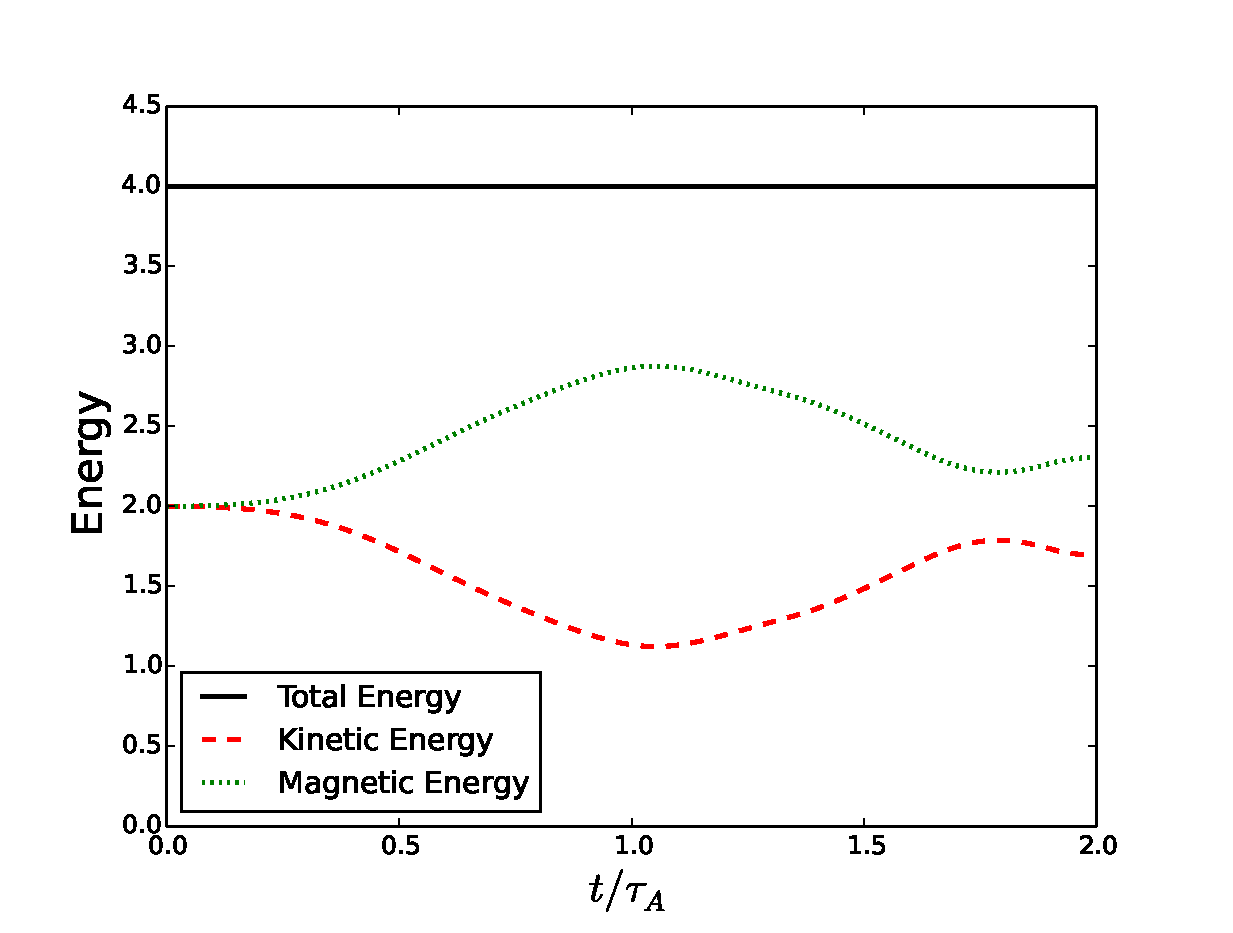
\includegraphics[width=14.8cm]{figs/gandalf/OT_energy.eps}
            \caption{Time evolution of kinetic and magnetic energies for the Orszag-Tang
            test case.}
            \label{gandalf:fig:OTenergy}
        \end{figure}

    \subsection{Turbulent spectra for Alfv\'{e}nic cascade}
    
    \begin{figure}
    \begin{center}
        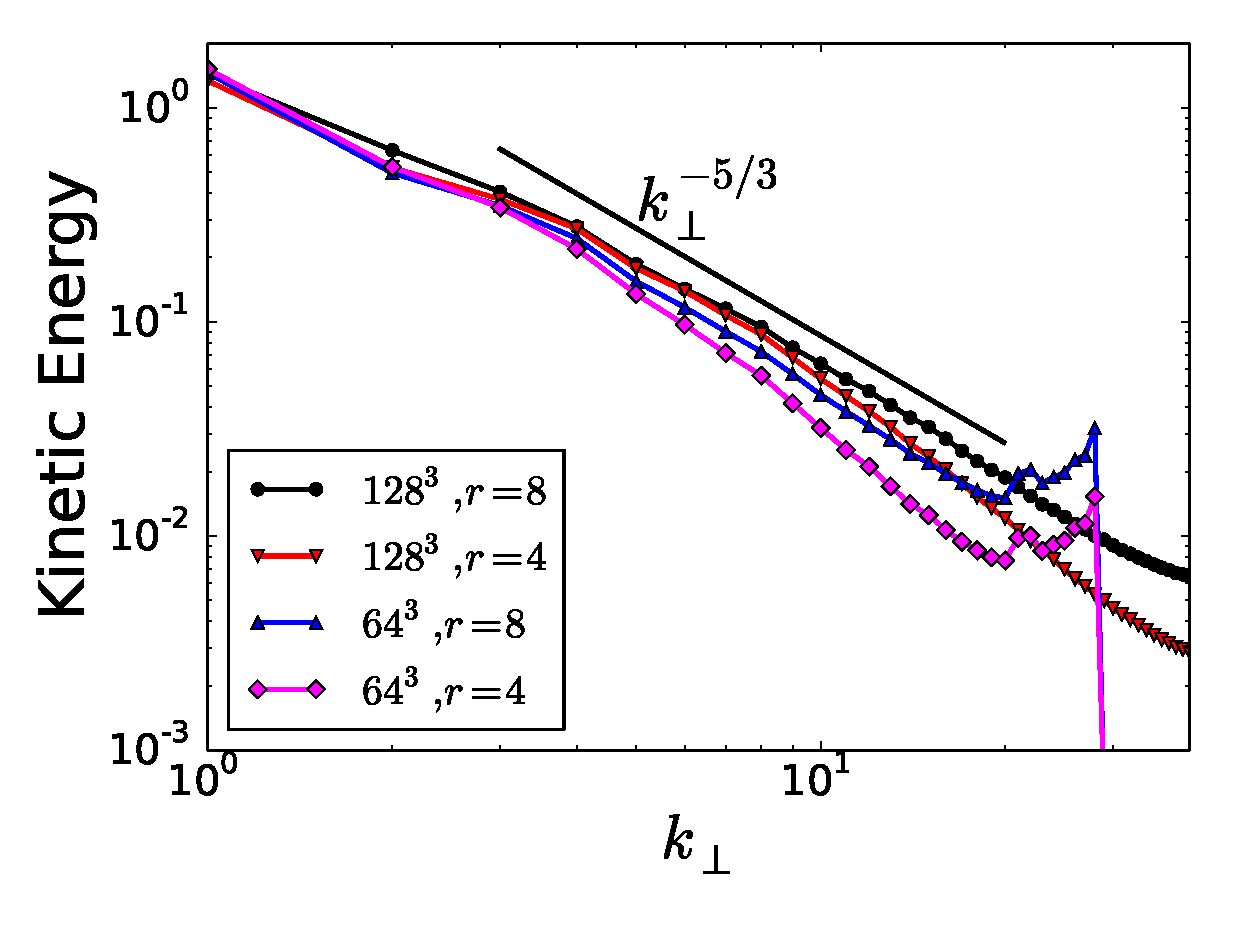
\includegraphics[width=7.4cm]{figs/gandalf/alfconv_KE.eps}
        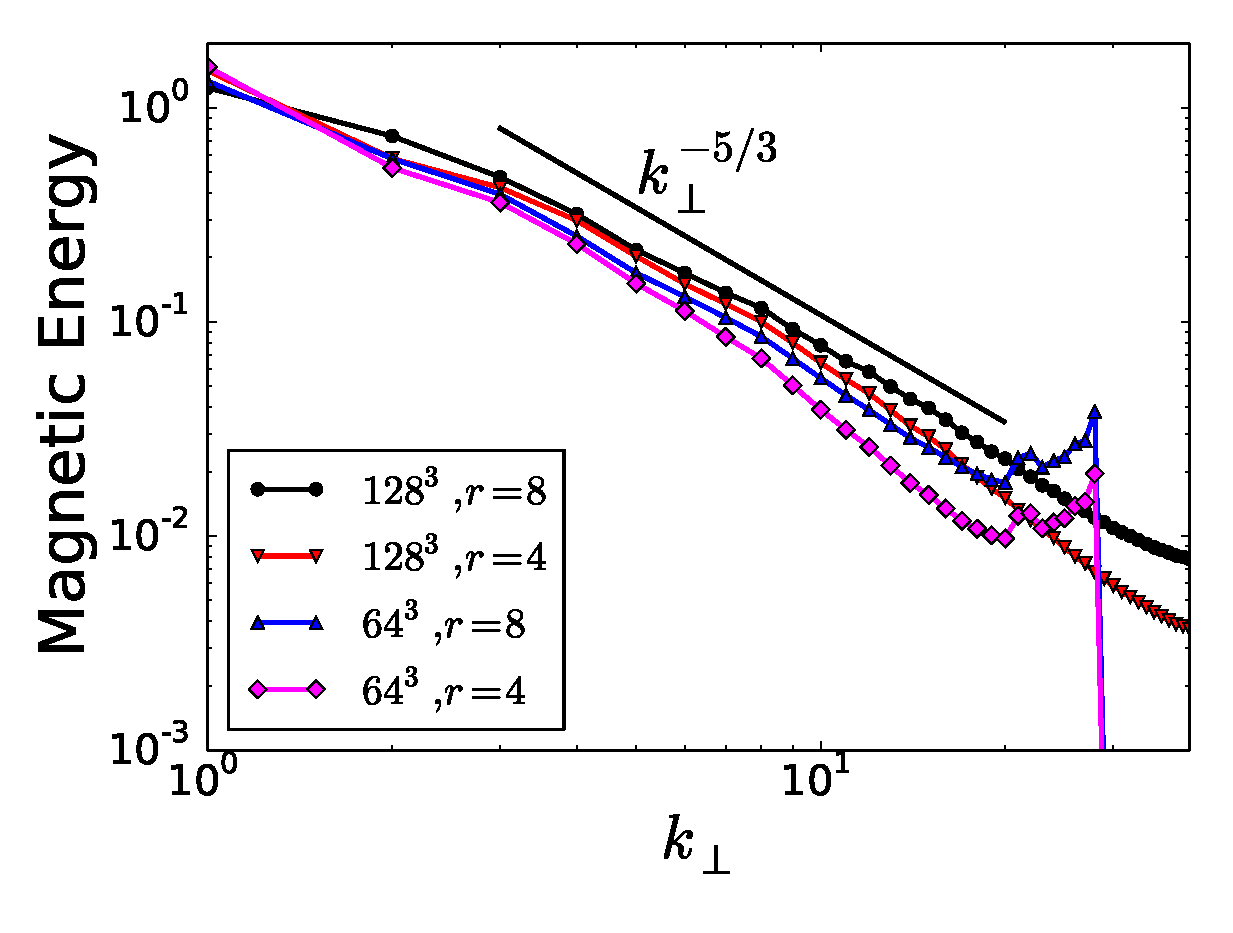
\includegraphics[width=7.4cm]{figs/gandalf/alfconv_ME.eps}
        \caption{The kinetic (left) and magnetic (right) energy spectra for Alfv\'{e}nic
        turbulent cascade. The four different lines correspond to four separate
        simulations---the first number is the resolution, and the second number is
        the exponent for the hyper-diffusion term (see \secref{gandalf:sec:hyper}). The
        spectra approach the critical-balance prediction of $k_\perp^{-5/3}$ for large
        resolution, and for large hyper-diffusion exponent.}
        \label{gandalf:fig:alfconv}
    \end{center}
    \end{figure}

    We simulated the reduced MHD equations for the simulation domains $64^3$, and $128^3$,
    with two different values for the hyper-diffusion exponent: $r=4$ and $r=8$. We ran
    these simulations till saturation, and then time-averaged the kinetic and magnetic
    energy spectra over two Alfv\'{e}n times. These time-averaged spectra are plotted in
    \figref{gandalf:fig:alfconv}---they are in agreement with the critical-balance prediction of
    $k_\perp^{-5/3}$.



%\renewcommand{\thechapter}{4}
\chapter{Fluctuation-dissipation relations for a kinetic Langevin equation}
\label{chap:phmixlin}
\section{Introduction}
Fluctuation dissipation relations (FDR) predict the response of a dynamical system to an externally 
applied perturbation, based on the system's internal dissipation properties. The classical Langevin
equation \cite{langevin1908, kubo66} supplies the best known example of such FDR. 
The standard formulation is to consider a scalar $\phi$ 
forced by a Gaussian white-noise source $\chi$ and damped at the rate $\gamma$: 
\begin{align}
&\pd{\phi}{t} + \gamma \phi  = \chi, \label{phmixlin:eq:Langevin} \\
&\la \chi(t) \chi(t') \ra  = \eps \delta (t-t'), \nonumber
\end{align}
where angle brackets denote the ensemble average and 
$\eps/2$ is the mean power injected into the system by the source:
\beq
\frac{\dd}{\dd t}\frac{\la\phi^2\ra}{2} + \gamma\la\phi^2\ra = \frac{\eps}{2}.  
\eeq
The steady-state mean square fluctuation level is then given by the FDR, linking 
the injection and the dissipation of the scalar fluctuations:    
\beq
\la \phi^2 \ra = \frac{\eps}{2\gamma}. 
\label{phmixlin:eq:FDR}
\eeq

The simplest physical example of such a system is a Brownian particle suspended 
in liquid, with $\phi$ the velocity of the particle and $\gamma$ the frictional damping.
More generally, \eqref{phmixlin:eq:Langevin} may be viewed as a generic model for 
systems where some perturbed quantity is randomly stirred and decays via 
some form of linear damping, a frequently encountered situation in, e.g., 
fluid dynamics. 

Nearly every problem in plasma physics involves a system with 
driven and damped linear modes. Here we consider the prototypical 
such case: the behavior of perturbations of a Maxwellian equilibrium 
in a weakly collisional plasma in one spatial and one velocity-space dimension.
In such a system (and in weakly collisional or collisionless plasmas generally), 
damping of the perturbed electric fields occurs via the famous Landau 
mechanism \cite{landau46}. Landau damping, however, is different in several respects from 
standard ``fluid'' damping phenomena. It is in fact a phase mixing process: 
electric---and, therefore, density---perturbations are phase mixed 
and thus are effectively damped (see \secref{intro:sec:phmix}). Their (free) energy is transferred 
to perturbations of the particle distribution function that develop 
ever finer structure in velocity space and are eventually removed by 
collisions or, in a formally collisionless limit, by some suitable coarse-graining procedure.  
The electrostatic potential $\phi$ in such systems cannot in general be 
rigorously shown to satisfy a ``fluid'' equation of the form \exref{phmixlin:eq:Langevin}, 
with $\gamma$ the Landau damping rate, although the idea that \eqref{phmixlin:eq:Langevin} 
or a higher-order generalization thereof 
is not a bad model underlies the so-called Landau-fluid closures 
\cite{hammett90,hammett92,hedrick92,dorland93,beer96,snyder97,snyder01,snyder01gf,passot04,goswami05,ramos05,passot06,passot07,passot12}. 

It is a natural question to ask whether, despite the dynamical equations
for $\phi$ (or, more generally, for the moments of the distribution function) 
being more complicated than \eqref{phmixlin:eq:Langevin}, we should still expect the 
mean fluctuation level to satisfy \eqref{phmixlin:eq:FDR}, where $\gamma$ is 
the Landau damping rate. And if that is not the case, then should the value of 
$\gamma$ {\em defined} by \eqref{phmixlin:eq:FDR} be viewed as the 
effective damping rate in a driven system, replacing the Landau rate? 
Plunk \cite{plunk13} recently considered the latter question
and argued that the fact that the effective damping rate defined this way 
differs from the Landau rate suggests a fundamental modification of Landau response 
in a stochastic setting. Our take on the problem at hand differs 
from theirs somewhat in that we take the kinetic version of the Langevin 
equation (introduced in \secref{phmixlin:sec:kin}) at face value and 
derive the appropriate kinetic generalization of the FDR, 
instead of attaching a universal physical significance to the ``fluid'' version of it. 
Interestingly, the kinetic FDR does simplify to the classical fluid FDR when 
the Landau damping rate is small. Furthermore, we prove that in this limit 
(and when the system has no real frequency), the dynamics of $\phi$ is in fact 
described by \eqref{phmixlin:eq:Langevin} 
with $\gamma$ equal precisely to the Landau rate (i.e., the simplest Landau fluid 
closure is a rigorous approximation in this limit). 
The latter result is obtained by treating the velocity-space dynamics 
of the system in Hermite space. We also show how phase mixing in our system can 
be treated as a free-energy flux in Hermite space, what form the FDR takes 
for the Hermite spectrum of the perturbations of the distribution function, 
and how collisional effects can be included. The intent of this treatment 
is to provide a degree of clarity as to the behavior of a very simple 
plasma model and thus set the stage for modelling more complex, nonlinear 
phenomena. 

In \secref{phmixlin:sec:kin}, 
we describe a simple model for a weakly collisional plasma, which we call the
kinetic Langevin equation, and then, in \secref{phmixlin:sec:FDR}, derive the FDR for the same, 
including the ``fluid'' limit mentioned above. In \secref{phmixlin:sec:Hermite}, 
Hermite-space dynamics are treated, including the limit where 
Landau-fluid closures hold rigorously.  
An itemized summary of our findings is given in \secref{phmixlin:sec:disc}. A version of the
calculation with a different random source is presented in \apref{ap:g1force}.

 
\section{Kinetic Langevin equation}
\label{phmixlin:sec:kin}

We consider the following (1+1)-dimensional model of a homogeneous plasma 
perturbed about a Maxwellian equilibrium: 
\begin{align}
&\pd{g}{t} + \underbrace{v\,\pd{g}{z}}_{\text{phase mixing}} 
+ \underbrace{v F_0 \pd{\phi}{z}}_{\text{electric field}} = 
\underbrace{\chi(t) F_0}_{\text{source}} +
\underbrace{C[g]}_{\text{collisions}}\!\!\!, \label{phmixlin:eq:g} \\
&\phi  = \alpha \int_{-\infty}^\infty \rmd v\, g, \label{phmixlin:eq:phi} \\
& \la \chi(t) \chi(t') \ra  = \eps \delta (t-t'), \nonumber
\end{align}
where $g(z,v,t)$ is the perturbed distribution 
function and $F_0(v)$ is the Maxwellian equilibrium distribution
$F_0=e^{-v^2}/\sqrt{\pi}$. The velocity $v$ (in the $z$ direction) 
is normalized to the thermal speed $\vth = \sqrt{2T/m}$ 
($T$ and $m$ are the temperature and mass of the particle species under consideration), 
spatial coordinate $z$ is normalized to an arbitrary length $L$, and time $t$ to $L/\vth$.
Only one species (either electrons or ions) is evolved. 
The second species follows the density fluctuations of the first via 
whatever response a particular physical situation warrants: 
Boltzmann, isothermal, or no response---all of these possibilities 
are embraced by \eqref{phmixlin:eq:phi}, which determines the (suitably normalized) 
scalar potential $\phi$ in terms of the perturbed density associated with~$g$; 
the parameter $\alpha$ contains all of the specific physics. 
For example, if $g$ is taken to be the perturbed ion distribution function 
in a low-beta magnetized plasma and electrons to have Boltzmann response, 
then $\alpha=ZT_e/T_i$, the ratio of the electron to ion temperatures ($Z$ is the ion charge in 
units of electron charge~$e$)---the resulting system describes (Landau-damped) ion-acoustic waves;
\eqref{phmixlin:eq:phi} in this case is the statement of quasineutrality. 
Another, even more textbook example is damped Langmuir waves, the case 
originally considered by Landau \cite{landau46}: $g$ is the perturbed electron distribution function, 
ions have no response, so $\alpha=2/k^2\lambda_{D}^2$, where 
$\lambda_{D}$ is the Debye length and $k$ is the wave number of the 
perturbation ($\dd/\dd z = ik$); \eqref{phmixlin:eq:phi} in this case is the Gauss-Poisson law. 

A particularly astrophysically and space-physically relevant example 
(in the sense of being accessible to measurements in the solar wind 
\cite{celnikier83,celnikier87,marsch90,bershadskii04,hnat05,chen11}) is 
the compressive perturbations in a magnetized plasma---perturbations 
of plasma density and magnetic-field strength at scales long compared 
to the ion Larmor radius (see KRMHD equations in \secref{intro:sec:krmhd}). The model
given by \eqsdash{phmixlin:eq:g}{phmixlin:eq:phi} can be obtained from KRMHD by setting the
Alfv\'{e}n fluctuations to zero, adding a source term, and defining the parameter $\alpha = -1/\Lambda$ (see
\eqref{intro:krmhd:Lambda}).

%These are in fact described 
%by two equations evolving two decoupled 
%functions $g^+$ and $g^-$, which are certain linear combinations 
%of the zeroth and second moments of the perturbed ion distribution 
%function with respect to the velocity perpendicular to the 
%mean magnetic field (taken to be in the $z$ direction). 
%These equations are derived in \cite[][\S 6.2.1]{tome} 
%and are of the form \exref{phmixlin:eq:g} with 
%\beq
%\alpha^\pm =-\lt[-\frac{T_i}{ZT_e} + \frac{1}{\beta_i}\pm A\rt]^{-1}, \quad
%A = \sqrt{\lt(1+\frac{T_i}{ZT_e}\rt)^2 + \frac{1}{\beta_i^2}} 
%\eeq
%for $g^\pm$, respectively (here $\beta_i=8\pi n_iT_i/B^2$ is the ion beta). 
%The physical fields, the density and magnetic-field-strength perturbations, are related 
%to $g^\pm$ by 
%\begin{align}
%\frac{\delta n}{n} &= \frac{1}{2A}\int\rmd v\lt[\lt(1 + \frac{T_i}{ZT_e} + \frac{1}{\beta_i} + A\rt)g^-
%- \frac{T_i}{ZT_e}\frac{2}{\beta_i}\,g^+\rt],\\
%\frac{\delta B}{B} &= \frac{1}{2A}\int\rmd v\lt[\lt(1 + \frac{T_i}{ZT_e} + \frac{1}{\beta_i} + A\rt)g^+
%- \lt(1+\frac{ZT_e}{T_i}\rt)g^-\rt].
%\end{align}
%While these expressions are perhaps not very physically transparent, it may aid 
%intuition to note that ${\delta n}/{n} \approx \int\rmd v g^-$ and 
%${\delta B}/{B} \approx \int\rmd v g^+$ either in the limit of 
%high $\beta_i$ and hot ions ($T_i\gg T_e$) or in the limit of 
%low $\beta_i$ and cold ions ($T_i\ll T_e$). At low $\beta_i$, the $g^-$ equation 
%describes ion-acoustic waves ($\alpha^-\approx ZT_e/T_i$; see above). 
%At high $\beta_i$, the $g^+$ equation describes a kinetic version of the MHD slow mode, 
%subject to a version of Landau damping due to \cite{barnes66}; 
%in this case, $\alpha^+\approx -1 + 1/\beta_i$. 
%
Thus, \eqsand{phmixlin:eq:g}{phmixlin:eq:phi} correspond a variety of interesting physical situations. 

The energy injection in \eqref{phmixlin:eq:g} is modelled by a white-in-time, Maxwellian-in-velocity-space 
source $\chi(t) F_0$ supplying fixed power $\propto \eps$ to the perturbations (see below). 
This is a direct analog of the noise term in the ``fluid'' Langevin equation
\exref{phmixlin:eq:Langevin}
and so this particular choice of forcing was made in order to enable the simplest possible
comparison with the ``fluid'' case\footnote{One might argue that this is not, however, 
the most physical form of forcing and that it would be better to inject energy 
by applying a random electric field to the plasma, rather than a source of density
perturbations. In \apref{ap:g1force} we present a version of our calculation for such a
more physical source, and show that all the key results are similar. Note that the forcing
in \eqref{phmixlin:eq:g} does not violate particle conservation because we assume that
spatial integrals of all perturbations vanish:
$\int\rmd z\, g = 0$, $\int\rmd z\,\chi = 0$.}.
The energy injection leads to sharp gradients in the velocity space (phase mixing), 
which are removed by the collision operator $C[g]$. 
``The energy'' in the context of a kinetic equation is the free energy of the 
perturbations \cite{schekochihin08,tome} (see \eqref{intro:eq:Wcomp}), given in this case by 
\beq
W = \int\rmd v\,\frac{\la g^2\ra}{2F_0} + \frac{\la\phi^2\ra}{2\alpha}
\label{phmixlin:eq:W}
\eeq    
and satisfying 
\beq
\frac{\rmd W}{\rmd t} = \frac{1+\alpha}{2}\,\eps + \int\rmd v\,\frac{g C[g]}{F_0}.
\label{phmixlin:eq:Wbalance}
\eeq
The first term on the right-hand side is the energy injection by the source, 
the second, negative definite term is its thermalization by collisions.
Note that the variance of $\phi$ is not by itself a conserved quantity:
\beq
\frac{\rmd}{\rmd t}\frac{\la\phi^2\ra}{2} + \alpha\lt\la\phi\frac{\dd}{\dd z}\int\rmd v\,vg\rt\ra 
= \frac{\alpha^2}{2}\,\eps.
\label{phmixlin:eq:phisq}
\eeq
The power $\alpha^2\eps/2$ injected into fluctuations of $\phi$ is 
transferred into higher moments of $g$ via phase mixing. 
Phase mixing is precisely this process of draining free energy 
from the lower moments and transferring it into higher moments of the 
distribution function---without collisions, this is just a redistribution 
of free energy within \eqref{phmixlin:eq:W}, which, in the absence of source, 
would look like a linear damping of $\phi$\footnote{Note that 
$\alpha=-1$ corresponds to an effectively undriven system; 
the Landau damping rate for this case is zero (\eqref{phmixlin:eq:omega_small}).
We will see in \secref{phmixlin:sec:KE_Hermite} that in this case the 
driven density moment decouples from the rest of the perturbed 
distribution function; see \eqref{phmixlin:eq:g1}. For $\alpha<-1$ the system 
is no longer a driven-damped system; this parameter regime never occurs 
physically.}.
 
In the presence of a source, the system described by \eqsand{phmixlin:eq:g}{phmixlin:eq:phi} 
is a driven-damped system much like the Langevin equation \exref{phmixlin:eq:Langevin}. 
The damping of $\phi$ in the kinetic case is provided by Landau damping 
(phase mixing) as opposed to the explicit dissipation term in \eqref{phmixlin:eq:Langevin}. 
It is an interesting question whether 
in the steady state, the second term on the left-hand side 
of \eqref{phmixlin:eq:phisq} can be expressed as $\geff\la\phi^2\ra$, leading 
an analogue of the FDR (\eqref{phmixlin:eq:FDR}), and if so, whether the 
``effective damping rate'' $\geff$ in this expression is equal 
to the Landau damping rate $\gamma_L$. 
The answer is that an analogue of the FDR does exist, 
$\geff$ is non-zero for vanishing collisionality, but in general, $\geff\neq\gamma_L$. 

\begin{figure}
\begin{center}
\includegraphics[width=14.8cm]{figs/phmixlin/phi2.eps}
\caption{Normalized steady-state amplitude $2\pi|k|\la|\phi_k|^2\ra/\eps_k=f(\alpha)$ 
vs.\ $1+\alpha$: the solid line is the analytical prediction 
($f(\alpha)$ as per \eqref{phmixlin:eq:f}), the crosses are computed from 
the long-time limit of $\la|\phi_k|^2\ra$ obtained via direct numerical 
solution of \eqsand{phmixlin:eq:g}{phmixlin:eq:phi}.}
\label{phmixlin:fig:f}
\end{center}
\end{figure}


\section{Kinetic Fluctuation-Dissipation Relations}
\label{phmixlin:sec:FDR}

Ignoring collisions in \eqref{phmixlin:eq:g} and Fourier-transforming it in space in time, 
we~get 
\beq
\gko = - \phiko\frac{v F_0}{v - \omega/k} - \frac{i\chiko}{k}\frac{F_0}{v - \omega/k}.
\label{phmixlin:eq:gko}
\eeq
Introducing the plasma dispersion function $Z(\zeta) = \int\rmd v F_0/(v-\zeta)$, 
where the integration is along the Landau countour \cite{fried61}, we find from 
\eqsand{phmixlin:eq:gko}{phmixlin:eq:phi}:
\begin{align}
\label{phmixlin:eq:phiko}
&\phiko = - \frac{i\chiko}{|k|}\frac{Z(\omega/|k|)}{D_\alpha(\omega/|k|)},\\
&D_\alpha\!\lt(\frac{\omega}{|k|}\rt) = 1 + \frac{1}{\alpha} + \frac{\omega}{|k|} Z\!\lt(\frac{\omega}{|k|}\rt).
\end{align}
Note that $D_\alpha(\omega/|k|) = 0$ is the dispersion relation for the classic Landau problem \cite{landau46}. 
We now inverse Fourier transform \eqref{phmixlin:eq:phiko} back into the time domain, 
\beq
\phi_k(t) = \int\rmd\omega\, e^{-i\omega t}\phiko = 
 - \frac{i}{|k|}\int\rmd\omega\, e^{-i\omega t}\chiko\frac{Z(\omega/|k|)}{D_\alpha(\omega/|k|)},
\eeq
and compute $\la|\phi_k|^2\ra$ 
in the steady state. In order to do this, we use the fact that 
$\chiko \equiv \int\rmd t e^{i\omega t}\chi_k(t)/2\pi$ satisfies 
$\la\chiko\chi^*_{k\omega'}\ra = \eps_k\delta(\omega-\omega')/2\pi$
because $\la\chi_k(t)\chi_k^*(t')\ra = \eps_k\delta(t-t')$, where 
$\eps_k$ is the source power at wave number $k$. 
The result is
\beq
\la|\phi_k|^2\ra = \frac{\eps_k}{2\pi|k|}f(\alpha),\quad 
f(\alpha) = \int_{-\infty}^{+\infty}\rmd\zeta\lt|\frac{Z(\zeta)}{D_\alpha(\zeta)}\rt|^2,
\label{phmixlin:eq:f}
\eeq
where we have changed the integration variable to $\zeta=\omega/|k|$. 
This is the fluctuation-dissipation relation for our kinetic system that predicts the
long-time behavior of the electrostatic potential. 
The function $f(\alpha)$, computed numerically as per \eqref{phmixlin:eq:f}, 
is plotted in \figref{phmixlin:fig:f}, together with the results of 
direct numerical solution of \eqsand{phmixlin:eq:g}{phmixlin:eq:phi}, in which $f(\alpha)$ 
is found by computing the saturated fluctuation level $\la|\phi_k|^2\ra$. 

\Eqref{phmixlin:eq:f} can be written in the form 
\beq
\la|\phi_k|^2\ra = \frac{\alpha^2\eps_k}{2\geff},\quad 
\geff(\alpha) = \frac{\pi\alpha^2}{f(\alpha)}|k|,
\label{phmixlin:eq:gamma}
\eeq  
but the ``effective damping rate'' $\geff$ is not in general the same 
as the Landau damping rate $\gamma_L$.
This is illustrated in \figref{phmixlin:fig:gamma_omega}, where we plot 
the real ($\omega_L$) and imaginary ($-\gamma_L$) parts of the slowest-damped root(s) 
of $D_\alpha(\omega/|k|) = 0$ 
together with $\geff(\alpha)$ for $\alpha<0$ and $\geff(\alpha)/2$ for $\alpha>0$. 
In the latter case, the linear modes of the system have real frequencies and 
the analogy with the Langevin equation \exref{phmixlin:eq:Langevin} is not apt---a better 
mechanical analogy is a damped oscillator, as explained at the end of 
\secref{phmixlin:sec:large}; the FDR in this case acquires an extra factor of $1/2$, which is 
why we plot $\geff/2$ (see \eqref{phmixlin:eq:FDR_osc}). Remarkably, $\geff(\alpha)$ does 
asymptote to $\gamma_L$ in the limit $1+\alpha\ll1$ and to $2\gamma_L$ in the limit 
$\alpha\to\infty$, i.e., when the damping is weak. 
These asymptotic results can be verified analytically. 

\begin{figure}
\begin{center}
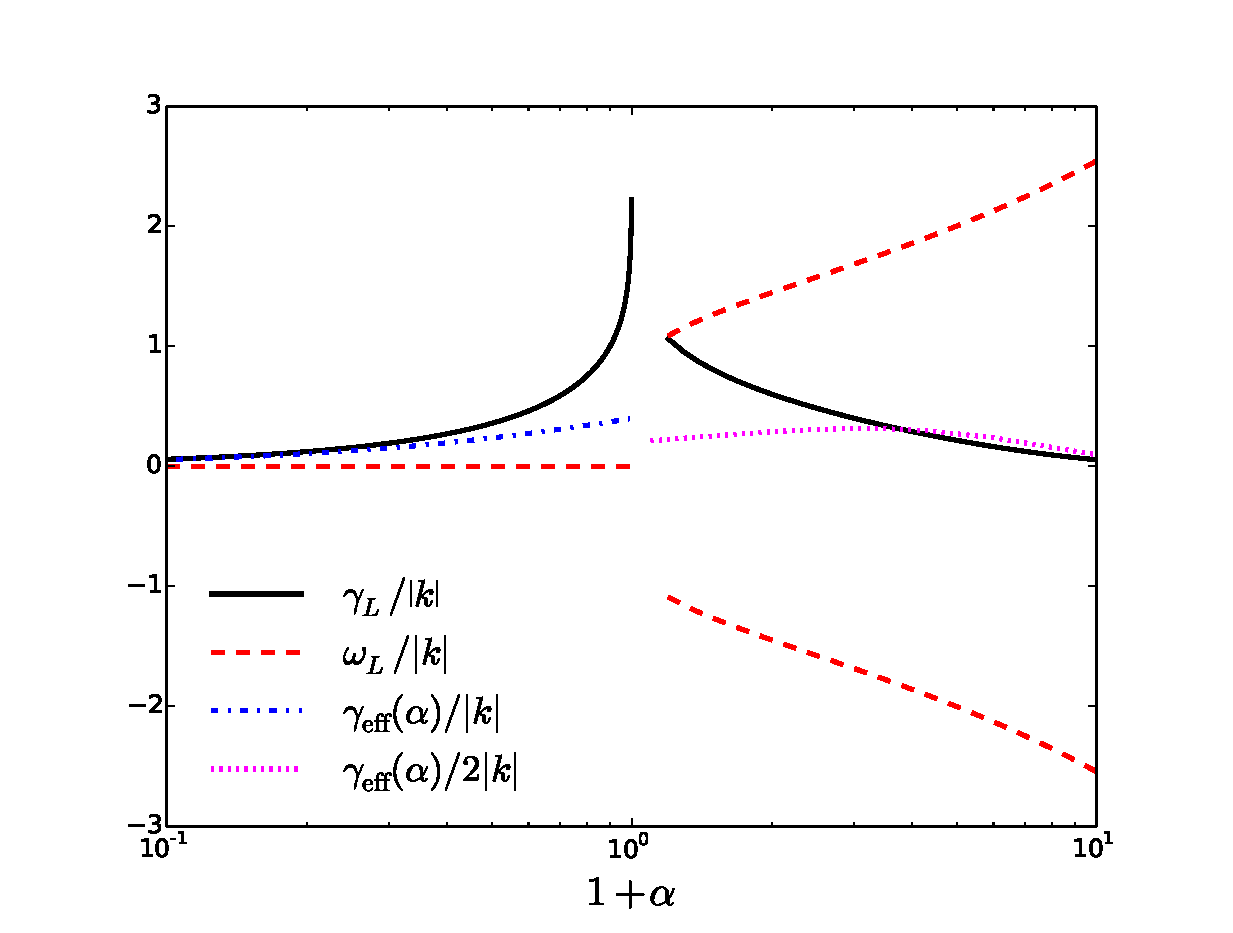
\includegraphics[width=14.8cm]{figs/phmixlin/gamma_omega.eps}
\caption{Slowest-damped solutions of the dispersion relation 
$D_\alpha(\omega/|k|)=0$: normalized frequency $\omega_L/|k|$ 
(red dashed line) and damping rate $\gamma_L/|k|$ (black soloid line)
vs.\ $1+\alpha$. Also shown are $\geff(\alpha)$ for $\alpha<0$ (blue dash-dotted 
line) and $\geff(\alpha)/2$ for $\alpha>0$ (magenta dotted line), as per 
\eqref{phmixlin:eq:gamma}. The two asymptotic limits in which these 
match $\gamma_L$ are discussed in \secsand{phmixlin:sec:small}{phmixlin:sec:large}.}
\label{phmixlin:fig:gamma_omega}
\end{center}
\end{figure}


\subsection{Zero real frequency, weak damping ($\alpha\to-1$)} 
\label{phmixlin:sec:small}

When $\alpha+1\ll1$, the solution of the dispersion relation will satisfy 
$\zeta~=~\omega/|k|~\ll~1$. In this limit, 
\beq
Z(\zeta)\approx i\sqrt{\pi},\quad
D_\alpha(\zeta)\approx 1 + \frac{1}{\alpha} + i\zeta\sqrt{\pi} 
\approx i\sqrt{\pi}\lt(\zeta - i\frac{1+\alpha}{\sqrt{\pi}}\rt).
\label{phmixlin:eq:Da_small}
\eeq
Therefore, the solution of $D_\alpha(\omega/|k|)=0$ is 
\beq
\omega \approx -i\gamma_L, \quad
\gamma_L = \frac{1+\alpha}{\sqrt{\pi}}|k|. 
\label{phmixlin:eq:omega_small}
\eeq
A useful physical example of Landau damping in this regime is the Barnes damping \cite{barnes66}
of compressive fluctuations in high-beta plasmas, where $1+\alpha\approx 1/\beta_i$ 
(see Schekochihin et al \cite{tome}, their eq.~(190)).

Since the zeros of $D_\alpha(\zeta)$ and $D_\alpha^*(\zeta)$, which are 
poles of the integrand in the expression for $f(\alpha)$ (\eqref{phmixlin:eq:f}), 
lie very close to the real line in this case, the integral is easily 
computed by using the approximate expressions \exref{phmixlin:eq:Da_small} for $Z(\zeta)$
and $D_\alpha(\zeta)$ and applying Plemelj's formula, to obtain 
\beq
f(\alpha) \approx \frac{\pi\sqrt{\pi}}{1+\alpha} = \frac{\pi|k|}{\gamma_L}
\quad\Rightarrow\quad
\la|\phi_k|^2\ra\approx \frac{\sqrt{\pi}\eps_k}{2(1+\alpha)|k|} = \frac{\eps_k}{2\gamma_L}.
\label{phmixlin:eq:FDR_small}
\eeq
Noting that $\alpha^2\approx1$, this is the same as 
\eqref{phmixlin:eq:gamma} with $\geff=\gamma_L$, so the ``fluid'' FDR is recovered.  
Note, however, that this recovery of the exact form of the ``fluid'' FDR 
is a property that is not universal with respect to the exact form of 
energy injection: as shown in \apref{ap:g1force}, it breaks down for 
a different forcing (see \eqref{phmixlin:eq:FDR_small1}).       


\subsection{Large real frequency, weak damping ($\alpha\to\infty$)} 
\label{phmixlin:sec:large}
 
Another analytically tractable limit is $\alpha\gg1$, in which case the solutions of the 
dispersion relation have $\zeta=\omega/|k|\gg1$. In this limit, 
\beq
Z(\zeta)\approx i\sqrt{\pi}\,e^{-\zeta^2} - \frac{1}{\zeta} - \frac{1}{2\zeta^3},\quad
D_\alpha(\zeta)\approx \frac{1}{\alpha} - \frac{1}{2\zeta^2} + i\sqrt{\pi}\,\zeta e^{-\zeta^2}.
\label{phmixlin:eq:Da_large}
\eeq
The solutions of $D_\alpha(\omega/|k|)=0$ are 
\beq
\omega \approx \pm\sqrt{\frac{\alpha}{2}}\,|k| - i\gamma_L,\quad
\gamma_L = \sqrt{\pi}\,\frac{\alpha^2}{4}\,e^{-\alpha/2}|k|.
\label{phmixlin:eq:omega_large}
\eeq
Two textbook examples of Landau-damped waves in this regime are 
ion acoustic waves at $\beta_i\ll1$, $T_i\ll T_e$ (cold ions), for which $\alpha=ZT_e/T_i$, 
and long-wavelength Langmuir waves, for which $\alpha = 2/k^2\lambda_D^2$ \cite{landau46}. 

In the integral in \eqref{phmixlin:eq:f}, the poles are again very close to the real line 
and so in the integrand, we may approximate, in the vicinity of one of the 
two solutions \exref{phmixlin:eq:omega_large} 
\beq
Z(\zeta) \approx \mp \sqrt{\frac{2}{\alpha}},\quad
D_\alpha(\zeta) \approx \pm \lt(\frac{2}{\alpha}\rt)^{3/2}\lt(\zeta \mp \sqrt{\frac{\alpha}{2}} + i\,\frac{\gamma_L}{|k|}\rt). 
\eeq
Using again Plemelj's formula and noting that equal contributions arise from each 
of the two roots, we find 
\beq
f(\alpha) \approx 2\sqrt{\pi}\,e^{\alpha/2} 
= \frac{\pi\alpha^2|k|}{2\gamma_L}
\quad\Rightarrow\quad
\la|\phi_k|^2\ra \approx \frac{\alpha^2\eps_k}{4\gamma_L}, 
\eeq
which is the same as \eqref{phmixlin:eq:gamma} with $\geff = 2\gamma_L$. 

Despite the apparently discordant factor of 2, this, in fact, is again 
consistent with a non-kinetic, textbook FDR. However, since we are considering a system with 
a large frequency, the relevant mechanical analogy is not \eqref{phmixlin:eq:Langevin}, but 
the equally standard (and more general) equation for a forced and damped oscillator: 
\beq
\ddot\phi + \gamma\dot\phi + \omega^2\phi = \dot\chi,
\label{phmixlin:eq:osc}
\eeq 
where overdots mean time derivatives.

We continue to consider $\chi$ a Gaussian white noise satisfying 
$\la\chi(t)\chi(t')\ra = \eps\delta(t-t')$.
For $\omega=0$, \eqref{phmixlin:eq:osc} then precisely reduces to \eqref{phmixlin:eq:Langevin}. 
For $\omega\neq0$, it is not hard to show (by Fourier transforming in time, 
solving, then inverse Fourier transforming and squaring the amplitude) that 
the stationary mean square amplitude $\la\phi^2\ra$ for \eqref{phmixlin:eq:osc} 
still satisfies \eqref{phmixlin:eq:FDR}. 
However, the relationship between the actual linear damping rate $\gamma_L$ 
of $\phi$ and the parameter $\gamma$ depends on the frequency: 
$\gamma_L = \gamma$ when $\omega\ll\gamma$ and $\gamma_L=\gamma/2$ when $\omega\ge\gamma/2$.  
In the latter case, which is the one with which we are preoccupied here, 
\eqref{phmixlin:eq:FDR} becomes, in terms of $\gamma_L$:  
\beq
\la\phi^2\ra = \frac{\eps}{4\gamma_L}.
\label{phmixlin:eq:FDR_osc}
\eeq
The required extra factor of 2 is manifest.\footnote{As in \secref{phmixlin:sec:small}, 
this very simple mechanical analogy also breaks down for a different choice of forcing; 
see \apref{ap:g1force} (\eqref{phmixlin:eq:FDR_large1}).}  


\section{Velocity-space structure}
\label{phmixlin:sec:Hermite}

The kinetic FDR derived in the previous section was concerned 
with the rate of removal of free energy from the density moment 
of the perturbed distribution function. This free energy flows into 
higher moments, i.e., is ``phase mixed'' away. In this section, 
we diagnose the velocity-space structure of the fluctuations
and extend the FDR to compute their amplitude. 

\subsection{Kinetic equation in Hermite space}
\label{phmixlin:sec:KE_Hermite}

The emergence of ever finer velocity-space scales is made explicit
by recasting the kinetic equation \exref{phmixlin:eq:g} in Hermite space, 
a popular approach for many years 
\cite{armstrong67,grant67a,hammett93,parker95,ng99,watanabe04,zocco11,loureiro13,hatch13,plunk14}. 
The distribution is decomposed into Hermite moments as follows
\beq
g(v) = \sum_{m=0}^\infty \frac{H_m (v) F_0 }{\sqrt{2^m m!}} g_m, \quad
g_m = \int \rmd v\, \frac{H_m(v)}{\sqrt{2^m m!}}\, g(v), 
\eeq
where $H_m(v)$ is the Hermite polynomial of order $m$. 
In terms of Hermite moments, \eqref{phmixlin:eq:phi} becomes
\beq
\phi = \alpha g_0,
\label{phmixlin:eq:phi_g0}
\eeq
while \eqref{phmixlin:eq:g} turns into a set of equations for the Hermite moments $g_m$, 
where phase mixing is manifested by the coupling of higher-$m$ moments 
to the lower-$m$ ones: 
\begin{align} 
\label{phmixlin:eq:g0}
&\pd{g_0}{t} + \pd{}{z}\frac{g_1}{\sqrt{2}}  = \chi,\\
\label{phmixlin:eq:g1}
&\pd{g_1}{t} + \pd{}{z}\lt(g_2 + \frac{1+\alpha}{\sqrt{2}}\,g_0\rt)  = 0,\\
&\pd{g_m}{t} + \pd{}{z}\lt(\sqrt{\frac{m+1}{2}}\,g_{m+1} + \sqrt{\frac{m}{2}}\,g_{m-1}\rt) 
= -\nu m g_m,  \quad m\ge2,
\label{phmixlin:eq:gmeq}
\end{align}
where $\nu$ is the collision frequency and 
we have used the \cite{lenard58} collision operator, a natural modelling 
choice in this context because its eigenfunctions are Hermite polynomials. 

The free energy \exref{phmixlin:eq:W} in these terms is 
\beq
W = \frac{1+\alpha}{2}\la g_0^2\ra + \frac{1}{2}\sum_{m=1}^\infty \la g_m^2\ra 
\eeq
and satisfies
\beq
\frac{\rmd W}{\rmd t} = \frac{1+\alpha}{2}\,\eps - \nu\sum_{m=2}^\infty m\la g_m^2\ra.
\label{phmixlin:eq:Wbal}
\eeq

\subsection{Fluctuation-Dissipation Relations in Hermite space}
\label{phmixlin:sec:FDR_Hermite}

It is an obvious generalization of the FDR to seek a relationship between 
the fluctuation level in the $m$-th Hermite moment, $\la|g_m|^2\ra$ 
(the ``Hermite spectrum''), and the injected power $\eps$.
This can be done in exactly the same manner as the kinetic FDR was 
derived in \secref{phmixlin:sec:FDR}. Hermite-transforming \eqref{phmixlin:eq:gko} gives   
\beq
\gmko = - \frac{i\chiko}{|k|}\frac{1+\alpha}{\alpha}\frac{(-\sgn k)^m}{\sqrt{2^m m!}}
\frac{Z^{(m)}(\omega/|k|)}{D_\alpha(\omega/|k|)},\quad m\ge1,
\label{phmixlin:eq:gm}
\eeq
where we have used 
\beq
Z^{(m)}(\zeta) \equiv \frac{\rmd^m Z}{\rmd\zeta^m} = 
(-1)^m\int\rmd v\,\frac{H_m(v) F_0(v)}{v-\zeta}
\label{phmixlin:eq:Zm}
\eeq
and $Z^{(m)}(\omega/k) = (\sgn k)^{m+1}Z^{(m)}(\omega/|k|)$. 
The mean square fluctuation level in the statistical steady state 
is then derived similarly to \eqref{phmixlin:eq:f}: 
\beq
\Cmk\equiv\la|\gmk|^2\ra = \frac{\eps_k}{2\pi|k|}\lt(\frac{1+\alpha}{\alpha}\rt)^2 
\frac{1}{2^m m!}\int_{-\infty}^{+\infty}\rmd\zeta\lt|\frac{Z^{(m)}(\zeta)}{D_\alpha(\zeta)}\rt|^2,
\quad m\ge1.
\label{phmixlin:eq:fm}
\eeq
This is the extension of the kinetic FDR, \eqref{phmixlin:eq:f}, to the fluctuations of the 
perturbed distribution function. The ``Hermite spectrum'' $\Cmk$ 
characterizes the distribution of free energy in phase space. 

\subsection{Hermite spectrum}
\label{phmixlin:sec:spectrum}

It is interesting to derive the asymptotic form of this spectrum at $m\gg1$. 
Using in \eqref{phmixlin:eq:Zm} the asymptotic form of the Hermite polynomials at large
$m$ \cite{abramowitz72},
\beq
e^{-v^2/2} H_m(v) \approx 
\lt(\frac{2m}{e}\rt)^{m/2}
\sqrt{2}\cos\lt(v\sqrt{2m} - \pi m/2\rt),
\label{phmixlin:eq:Hm}
\eeq
and remembering that the $v$ integration is over the Landau contour 
(i.e., along the real line, cicumnavigating the pole at $v=\zeta$ from below), 
we find
\beq
Z^{(m)}(\zeta) \approx i^{m+1}\sqrt{2\pi}\lt(\frac{2m}{e}\rt)^{m/2}e^{-\zeta^2/2 + i\zeta\sqrt{2m}},
\label{phmixlin:eq:Zm_approx}
\eeq 
provided $\zeta\ll\sqrt{2m}$ (this result is obtained by expressing the cosine 
in \eqref{phmixlin:eq:Hm} in terms of exponentials, completing the square in the
exponential function appearing in the integral \exref{phmixlin:eq:Zm} and moving 
the integration contour to $v = \pm i\sqrt{2m}$; the dominant contribution 
comes from the Landau pole). Finally, in \eqref{phmixlin:eq:fm}, 
\beq
\frac{|Z^{(m)}(\zeta)|^2}{2^m m!} \approx \sqrt{\frac{2\pi}{m}}\, e^{-\zeta^2},
\eeq
and so the Hermite spectrum has a universal scaling at $m\gg1$:
\beq
\Cmk \approx \lt[\frac{\eps_k}{\sqrt{2\pi}|k|}\lt(\frac{1+\alpha}{\alpha}\rt)^2 
\int_{-\infty}^{+\infty}\frac{\rmd\zeta\,e^{-\zeta^2}}{|D_\alpha(\zeta)|^2}\rt]\frac{1}{\sqrt{m}}
=\frac{\eps_k (1+\alpha)}{\sqrt{2 } |k|} \frac{1}{\sqrt{m}}.
\label{phmixlin:eq:Cuniv}
\eeq
The universal $1/\sqrt{m}$ scaling was derived in a different way by Zocco et al.\cite{zocco11} 
(see \secref{phmixlin:sec:flux}; \cite{watanabe04,hatch13}). 
The integral in \exref{phmixlin:eq:Cuniv} was evaluated using the Kramers--Kronig relations 
\cite{kramers27,kronig26} for the function
$h(\zeta) = 1/D_\alpha(\zeta) - \alpha$ 
(which is analytic in the upper half plane and decays at least as fast as $1/|\zeta|^2$ at large $\zeta$):
\beq
\int_{-\infty}^{+\infty}\frac{\rmd\zeta\,e^{-\zeta^2}}{|D_\alpha(\zeta)|^2} = 
-\sqrt{\pi}
\lt[\frac{1}{\pi}\,
{\cal P}\int_{-\infty}^{+\infty}\frac{\rmd\zeta\,\Imag\, h(\zeta)}{\zeta - \zeta'}\rt]_{\zeta'=0} 
= -\sqrt{\pi}\, \Real\, h(0) = \frac{\alpha^2}{1+\alpha}\sqrt{\pi}.
\eeq
Note that 
in the limit of high frequency ($\alpha\gg1$, \secref{phmixlin:sec:large}), 
the approximation \exref{phmixlin:eq:Zm_approx} requires $\omega_L/|k|\ll\sqrt{2m}$, or $\alpha\ll4m$,  
but there is also a meaningful intermediate range of $m$ for which 
$1\le m \ll \alpha/4$. In this range, we 
can approximate $Z(\zeta)\approx -1/\zeta$ and, since $\zeta\approx\pm\sqrt{\alpha/2}$, 
we have in \eqref{phmixlin:eq:fm}:
\beq
\frac{|Z^{(m)}(\zeta)|^2}{2^m m!} \approx \frac{2m!}{\alpha^{m+1}}
\quad\Rightarrow\quad
\Cmk \approx \frac{\eps_k}{\sqrt{\pi}|k|}\frac{m!}{\alpha^m}\,e^{\alpha/2}.
\eeq
This spectrum decays with $m$ up to $m\sim\alpha$, where it 
transitions into the universal spectrum \exref{phmixlin:eq:Cuniv}.

\subsection{Free-energy flux, the effect of collisions and the FDR for the total free energy}
\label{phmixlin:sec:flux}

Observe that the total free energy in our system, with its $1/\sqrt{m}$ 
Hermite spectrum, is divergent. The regularization in Hermite space 
(removal of fine velocity-space scales) is provided by collisions. 
If $\nu$ is infinitesimal, these are irrelevant at finite $m$, 
but eventually become important as $m\to\infty$. To take account 
of their effect and to understand the free-energy flow in 
Hermite space, we consider \eqref{phmixlin:eq:gmeq}, which it is convenient 
to Fourier transform in $z$ and rewrite in terms of 
$\tgmk \equiv (i\,\sgn k)^m\gmk$: 
\beq
\pd{\tgmk}{t} + \frac{|k|}{\sqrt{2}}\lt(\sqrt{m+1}\,\tg_{m+1,k} - \sqrt{m}\,\tg_{m-1,k}\rt) 
= - \nu m\tgmk. 
\label{phmixlin:eq:tg}
\eeq
The Hermite spectrum $\Cmk=\la|\gmk|^2\ra =\la|\tgmk|^2\ra$ therefore satisfies 
\beq
\pd{\Cmk}{t} + \Gamma_{m+1/2,k} - \Gamma_{m-1/2,k} = - 2\nu m \Cmk,
\label{phmixlin:eq:Cmk_exact}
\eeq
where $\Gamma_{m+1/2,k} = |k|\sqrt{2(m+1)}\Re\la\tg_{m+1,k}\tgmk^*\ra$ is the 
free-energy flux in Hermite space. If we make an assumption 
(verified in \secref{phmixlin:sec:cont})
that for $m\gg1$ the Hermite moments $\tgmk$ are continuous in $m$, i.e., 
$\tg_{m+1,k}\approx\tgmk$, then 
\beq
\Gamma_{m+1/2,k}\approx |k|\sqrt{2(m+1)}\,C_{m+1,k}
\label{phmixlin:eq:Gamma_cont}
\eeq
and \eqref{phmixlin:eq:Cmk_exact} turns into a closed evolution equation for the 
Hermite spectrum \cite{zocco11}: 
\beq
\pd{\Cmk}{t} + |k|\pd{}{m}\sqrt{2m}\,\Cmk = - 2\nu m \Cmk.
\label{phmixlin:eq:Cmk_approx}
\eeq
The universal $\Cmk\propto 1/\sqrt{m}$ spectrum derived in \secref{phmixlin:sec:spectrum} 
is now very obviously a constant-flux spectrum, reflecting steady 
pumping of free energy towards higher $m$'s (phase mixing). 
The full steady-state solution of 
\eqref{phmixlin:eq:Cmk_approx} including the collisional cutoff is 
\beq
\Cmk = \frac{A_k}{\sqrt{m}}\,\exp\lt(-\frac{2\sqrt{2}}{3}\frac{\nu}{|k|}m^{3/2}\rt),
\label{phmixlin:eq:Ccoll}
\eeq
where $A_k$ is an integration constant, which must be determined by matching 
this high-$m$ solution with the Hermite spectrum at low $m$. This we are now 
in a position to do: for $1\ll m\ll (\nu/|k|)^{-2/3}$, $\Cmk\approx A_k/\sqrt{m}$ 
and comparison with \eqref{phmixlin:eq:Cuniv} shows that the constant $A_k$ is the 
same as the constant $A_k(\alpha)$ in that equation. Thus, \eqref{phmixlin:eq:Ccoll} 
with $A_k$ given by \eqref{phmixlin:eq:Cuniv} provides a uniformly valid 
expression for the Hermite-space spectrum, including the collisional cutoff
(modulo the Hermite-space continuity assumption \exref{phmixlin:eq:Gamma_cont}, 
which we will justify in \secref{phmixlin:sec:cont}).  

As a check of consistency of our treatment, let us calculate 
the collisional dissipation rate of the free energy. 
This is the second term on the right-hand side of \eqref{phmixlin:eq:Wbal}. 
Since $\Cmk\propto1/\sqrt{m}$ before the collisional cutoff is reached, 
the sum over $m$ will be dominated by $m\sim(\nu/|k|)^{-2/3}$ 
and can be approximated by an integral: 
\beq
\nu\sum_{m,k} m\Cmk \approx \sum_k \nu\int_0^\infty\rmd m\,m\Cmk 
= \sum_k \frac{A_k|k|}{\sqrt{2}}. 
\eeq
On the other hand, in steady state, \eqref{phmixlin:eq:Wbal} implies 
\beq
\nu\sum_{m,k} m\Cmk = \frac{1+\alpha}{2}\,\eps. \label{phmixlin:eq:Wbal_stst}
\eeq
If energy injection is into a single $k$ mode, $\eps=\eps_k$,  
comparing these two expressions implies 
\beq
A_k = \frac{\eps_k (1+\alpha)}{\sqrt{2}|k|}, 
\label{phmixlin:eq:Ak}
\eeq
which, of course, is consistent with \eqref{phmixlin:eq:Cuniv}.

Finally, we use \eqref{phmixlin:eq:Ccoll} to calculate (approximately) 
the total steady-state amount of free energy across the phase space:
\beq
\frac{1}{2}\sum_{m=1}^\infty \Cmk 
= \frac{\Gamma(1/3)}{\sqrt{2}\,3^{2/3}}\frac{A_k}{(\nu/|k|)^{1/3}}
= \frac{\Gamma(1/3)}{2\cdot3^{2/3}}\frac{1+\alpha}{\nu^{1/3}|k|^{2/3}}\,\eps_k
\label{phmixlin:eq:Wtot}
\eeq
(we have again approximated the sum with an integral, 
assumed energy injection into a single $k$ and used \eqref{phmixlin:eq:Ak}). 
\Eqref{phmixlin:eq:Wtot} can be thought of as the FDR for the total free energy.  
The fact that this diverges as $\nu\to 0$ 
underscores the principle that the ``true'' dissipation (in the sense of free 
energy being thermalized) is always collisional---a consequence of Boltzmann's 
$H$ theorem.  

\subsection{Continuity in Hermite space}
\label{phmixlin:sec:cont}

In this section, we make a somewhat lengthy formal digression to 
justify the assumption of continuity of Hermite moments in $m$ at 
large $m$, which we need for the approximation \exref{phmixlin:eq:Gamma_cont}. 
The formalism required for this will have some interesting features 
which are useful in framing one's thinking about energy flows in 
Hermite space. 

Returning to \eqref{phmixlin:eq:tg} and considering $1\ll m\ll (\nu/|k|)^{-2}$, 
we find that to lowest approximation, the $\sqrt{m}$ terms are dominant 
and must balance, giving $\tg_{m+1,k}\approx\tg_{m-1,k}$. 
This is consistent with continuity in $m$, viz., $\tg_{m+1,k}\approx\tg_{m,k}$, 
but there is also a solution allowing the consecutive Hermite 
moments to alternate sign: $\tg_{m+1,k}\approx-\tgmk$. 
Thus, there are, formally speaking, two solutions: one for which 
$\tgmk$ is continuous and one for which $(-1)^m\tgmk$ is. To take into account 
both of them, we introduce the following decomposition 
\cite{schekochihin14}: 
\beq
\tgmk = \tgmk^+ + (-1)^m\tgmk^-,
\label{phmixlin:eq:decomp}
\eeq
where the ``$+$'' (``continuous'') and the ``$-$'' (``alternating'') modes are
\beq
\tgmk^+ = \frac{\tgmk + \tg_{m+1,k}}{2}, \quad
\tgmk^- = (-1)^m\frac{\tgmk - \tg_{m+1,k}}{2}.
\label{phmixlin:eq:gpm}
\eeq
The Hermite spectrum and the flux of the free energy can be expressed 
in terms of the spectra of these modes as follows: 
\begin{align}
&\Cmk \equiv \la|\tgmk|^2\ra = \Cmk^+ + \Cmk^-, \label{phmixlin:eq:free_energy}\\
&\Gamma_{m+1/2,k} \equiv |k|\sqrt{2(m+1)}\Re\la\tg_{m+1,k}\tgmk^*\ra 
\approx |k|\sqrt{2m}\lt(\Cmk^+ - \Cmk^-\rt),
\label{phmixlin:eq:Gamma_pm}
\end{align}
where $\Cmk^\pm\equiv \la|\tgmk^\pm|^2\ra$ and the last expression 
in \eqref{phmixlin:eq:Gamma_pm} is an approximation valid for $m\gg1$. 

The functions $\tgmk^\pm$ can both be safely treated as continuous in $m$ for $m\gg1$. 
Treating them so in \eqref{phmixlin:eq:tg} and working to lowest order in $1/m$, 
we find that they satisfy the following {\em decoupled} evolution equations: 
\beq
\pd{\tgmk^\pm}{t} \pm \sqrt{2}|k| m^{1/4}\pd{}{m} m^{1/4}\tgmk^\pm = - \nu m\tgmk^\pm,
\label{phmixlin:eq:gpmevol}
\eeq 
or, for their spectra, 
\beq
\pd{\Cmk^\pm}{t} \pm |k|\pd{}{m}\sqrt{2m}\,\Cmk^\pm = - 2\nu m \Cmk^\pm.
\eeq
Manifestly, the ``$+$'' mode propagates from lower to higher $m$ and 
the ``$-$'' mode from higher to lower $m$---they are the ``phase-mixing'' and 
the ``un-phase-mixing'' collisionless solutions, respectively.\footnote{The existence 
of un-phase-mixing solutions has been known for a long time: e.g., 
\cite{hammett93} treated them as forward and backward propagating 
waves in a mechanical analogy of \eqref{phmixlin:eq:tg} with a row of masses 
connected by springs. The un-phase mixing solutions are also 
what allows the phenomenon of plasma echo \cite{gould67}, including 
in stochastic nonlinear systems \cite{schekochihin14}.}

Taking the collisional term into account and noting that energy is injected 
into the system at low, rather than high, $m$, the solution satisfying 
the boundary condition $\tgmk\to 0$ as $m\to\infty$ has $\tgmk^-=0$
and so $\tgmk=\tgmk^+$. Thus, $\tgmk$ is continuous in $m$. 
With $\Cmk^-=0$, \eqref{phmixlin:eq:Gamma_pm} is the same as our earlier 
approximation \exref{phmixlin:eq:Gamma_cont} (to lowest order in the $m\gg1$ expansion). 

As $\tgmk^+$ and $\tgmk^-$ are decoupled at large $m$, if we start with a 
$\tgmk^-=0$ solution, no $\tgmk^-$ will be produced. 
However, both the decoupling property and the interpretation of 
$\tgmk^\pm$ as the phase-mixing and un-phase-mixing modes
are only valid to lowest order in $1/m$. It is useful 
to know how well this approximation holds. 

\begin{figure}
\begin{center}
\includegraphics[width=14.8cm]{figs/phmixlin/Cpm.eps}
\caption{The free-energy spectra $C_m^\pm$ obtained via direct numerical solution 
of \eqsdash{phmixlin:eq:g0}{phmixlin:eq:gmeq} with $\alpha = 1.0$ followed by decomposing the solution 
according to \eqref{phmixlin:eq:gpm}. In the code, rather than using the Lenard--Bernstein 
collision operator (as per \eqref{phmixlin:eq:gmeq}), hypercollisional regularization, $-\nu m^6\gmk$, was used to maximize the utility of the velocity-space resolution, 
hence the very sharp cut off. 
The dotted lines show the collisionless approximation: \eqref{phmixlin:eq:Cuniv} 
for $\Cmk^+$ (the phase-mixing ``$+$'' mode predominates, so 
$\Cmk\approx\Cmk^+$) and \eqref{phmixlin:eq:Cminus} for $\Cmk^-$.} 
\label{phmixlin:fig:Cpm}
\end{center}
\end{figure}

Let us use \eqref{phmixlin:eq:gm} to calculate (in the collisionless limit) 
\beq
R_{m+1} \equiv \frac{\tg_{m+1,k\omega}}{\tgmko} = 
i\,\sgn k\,\frac{g_{m+1,k\omega}}{\gmko} 
= -\frac{i}{\sqrt{2(m+1)}}\frac{Z^{(m+1)}(\zeta)}{Z^{(m)}(\zeta)}.
\label{phmixlin:eq:Rm_exact}
\eeq
Taking $m\gg1, \zeta^2/4$ and using \eqref{phmixlin:eq:Zm_approx}, we find\footnote{The same 
lowest-order expression can be found by Fourier-transforming 
\eqref{phmixlin:eq:tg} in time, ignoring collisions, 
writing $R_{m+1} = R_m^{-1}\sqrt{m/(m+1)} + i\zeta\sqrt{2/(m+1)}$, 
approximating $R_m\approx R_{m+1}$, solving the resulting quadratic equation for $R_{m+1}$,  
expanding in powers of $1/\sqrt{m}$ and choosing the solution for which $R_{m+1}=1$ 
to lowest order. This last step is the main difference between the two methods: 
if we work with \eqref{phmixlin:eq:tg} in the manner just described, we have to make an explicit 
choice between the continuous and alternating solutions ($R_{m+1}=1$ and $R_{m+1}=-1$); 
on the other hand, \eqref{phmixlin:eq:gm} already contains the choice of the former (which is ultimately 
traceable to Landau's prescription guaranteeing damping rather than growth of the perturbations).}
\beq
R_{m+1} = 1 + \frac{i\zeta}{\sqrt{2m}} - \frac{1}{4m} + O\lt(\frac{1}{m^{3/2}}\rt).
\label{phmixlin:eq:Rm_approx}
\eeq
Therefore, to lowest order in $1/\sqrt{m}$, 
\beq
\tgmko^- = (-1)^m\tgmko\,\frac{1-R_{m+1}}{2} 
\approx(-1)^{m+1}\,\frac{i\zeta}{2\sqrt{2m}}\,\tgmko. 
\eeq
Following the same steps as those that led to \eqref{phmixlin:eq:Cuniv}\footnote{The integral is 
again calculated via Kramers--Kronig relations, this time for the function 
$h(\zeta) = \zeta^2/D_\alpha(\zeta) - \alpha \zeta^2 - \alpha^2/2$, 
so $\int_{-\infty}^{+\infty}\rmd\zeta\,\zeta^2 e^{-\zeta^2}\!/|D_\alpha(\zeta)|^2
= \alpha^2\sqrt{\pi}/2$.}, 
we get
\beq
\Cmk^- \approx \lt[\frac{\eps_k}{8\sqrt{2\pi}|k|}\lt(\frac{1+\alpha}{\alpha}\rt)^2 
\int_{-\infty}^{+\infty}\frac{\rmd\zeta\,\zeta^2
e^{-\zeta^2}}{|D_\alpha(\zeta)|^2}\rt]\frac{1}{m^{3/2}} 
 = \frac{\eps_k (1+\alpha)^2}{16 \sqrt{2} |k|} \frac{1}{m^{3/2}}, 
\label{phmixlin:eq:Cminus}
\eeq
so both the energy ($\sim 1$, while the total is $\sim\nu^{-1/3}$; see \eqref{phmixlin:eq:Wtot})
and the dissipation ($\sim\nu\sum_m m\Cmk^-\sim \nu^{2/3}$) associated with the 
``$-$'' modes is small.  

The steady-state spectra $\Cmk^\pm$ obtained via direct numerical solution 
of \eqsand{phmixlin:eq:g}{phmixlin:eq:phi} are shown in \figref{phmixlin:fig:Cpm}, where they are also 
compared with the analytical expressions \exref{phmixlin:eq:Cuniv} and \exref{phmixlin:eq:Cminus}.  

Note that we could have, without further ado, simply taken 
\eqref{phmixlin:eq:Rm_approx} to be the proof of continuity in Hermite space. We have chosen 
to argue this point via the decomposition \exref{phmixlin:eq:decomp} because it provided 
us with a more intuitive understanding of the connection between this continuity 
and the direction of the free-energy flow (phase mixing rather than un-phase mixing). 

\subsection{The simplest Landau-fluid closure}
\label{phmixlin:sec:LF}

Simplistically described, the idea of Landau-fluid closures 
is to truncate the Hermite hierarchy of \eqsdash{phmixlin:eq:g0}{phmixlin:eq:gmeq} 
at some finite $m$ and to replace in the last retained equation
\beq
g_{m+1,k}(t) = -(i\,\sgn k) R_{m+1}\gmk(t),
\label{phmixlin:eq:trunc}
\eeq
where $R_{m+1}$, which in general depends on the complex frequency $\zeta$ (\eqref{phmixlin:eq:Rm_exact}),
is approximated by some suitable frequency-independent expression leading 
to the correct recovery of the linear physics from the truncated system.   
A considerable level of sophistication has been achieved in making these choices 
and we are not proposing to improve on the existing literature 
\cite{hammett90,hammett92,hedrick92,dorland93,snyder97,passot04,goswami05,passot07}. 
It is, however, useful, in the context of the result of \secref{phmixlin:sec:small} that 
the ``fluid'' version of FDR is recovered in the limit of low frequency and weak 
damping, to show how the same conclusion can be arrived at via what is probably 
the simplest possible Landau-fluid closure. 

In the limit $\zeta\to0$, the ratio $R_{m+1}$, given by \eqref{phmixlin:eq:Rm_exact}, becomes 
independent of $\zeta$ and so a closure in the form \exref{phmixlin:eq:trunc} 
becomes a rigorous approximation. It is not hard to show that 
\beq
Z^{(m)}(0) = \frac{i^{m+1}\sqrt{\pi}\, m!}{\Gamma(m/2 + 1)}.
\eeq
Therefore, for $\zeta\ll1$ and $m\ge1$,\footnote{The same result can be obtained 
by inferring $R_{m+1} \approx R_m^{-1}\sqrt{m/(m+1)}$ from \eqref{phmixlin:eq:tg} 
(provided $m\ll1/\zeta^2$), then iterating this up to some Hermite number $M$
such that $1\ll M\ll1/\zeta^2$, and approximating $R_M\approx1$ (\eqref{phmixlin:eq:Rm_approx}).
The condition $m, M \ll 1/\zeta^2$ is necessary so that the $\zeta$ terms in 
$R_{m+1}$ are not just small compared to unity but also compared to the next-order 
$1/m$ terms (see \eqref{phmixlin:eq:Rm_approx}).} 
\beq
R_{m+1} = \frac{m}{\sqrt{2(m+1)}}\frac{\Gamma(m/2)}{\Gamma((m+1)/2)}. 
\eeq
If we wish to truncate at $m=1$, then $R_2=\sqrt{\pi}/2$, and so in \eqref{phmixlin:eq:g1}, 
\beq
g_{2,k}=-i\,\sgn k\,\frac{\sqrt{\pi}}{2}\,g_{1,k}.
\eeq
On the basis of \eqref{phmixlin:eq:g0}, we must order $g_{1,k}\sim O(\zeta) g_{0,k}$. 
Thefore, $\dd g_{1,k}/\dd t \sim O(\zeta^2) g_{0,k}$ must be neglected 
in \eqref{phmixlin:eq:g1}, from which we then learn that 
\beq
g_{1,k}\approx -i\,\sgn k\,\sqrt{\frac{2}{\pi}}\lt(1+\alpha\rt) g_{0,k}.
\eeq
Finally, substituting this into \eqref{phmixlin:eq:g0}, we get
\beq
\pd{g_{0,k}}{t} + \frac{1+\alpha}{\sqrt{\pi}}|k| g_{0,k} = \chi_k.
\label{phmixlin:eq:LF_Langevin}
\eeq
This is a Langevin equation \exref{phmixlin:eq:Langevin} with a damping rate that 
is precisely the Landau damping rate $\gamma_L$ in the limit $1+\alpha\ll1$ 
(and so $\zeta\ll1$), given by \eqref{phmixlin:eq:omega_small}. 
In this limit, $\phi = -g_0$ (\eqref{phmixlin:eq:phi_g0}, $\alpha\approx-1$) 
and we recover the standard ``fluid'' FDR (\eqref{phmixlin:eq:FDR_small}). 
As we discussed in \secref{phmixlin:sec:kin}, a useful application of this regime 
is to compressive fluctuations in high-beta plasmas: in this case 
$1+\alpha\approx 1/\beta_i\ll1$ and the damping is the Barnes damping (also known as
transit-time damping) \cite{barnes66}, well known in space and astrophysical contexts \cite{foote79,lithwick01,tome}. 


\section{Conclusions and discussion}
\label{phmixlin:sec:disc}

We have provided a reasonably complete treatment 
of the simplest generalization of the Langevin problem to plasma kinetic 
systems. While we have focused on the simplest Langevin problem, in which the 
source term is a white noise, there is an obvious route towards generalizing 
this by considering source terms with more coherent time dependence 
(longer correlation times, prescribed frequency spectra; see \cite{plunk13}). 
One such calculation was recently undertaken by Plunk \cite{plunk14}, who 
considered a coherent oscillating source and found
that when the frequency of the source is large, the amount of energy that 
can be absorbed by the kinetic system is exponentially small. 
Another straightforward generalization (or variation) of our model
(as treated in this chapter) 
is energy injection into momentum, rather than density fluctuations---which can 
be interpreted as forcing by an externally imposed random electric field.
Whereas some of the more literal parallels with the Langevin problem 
are lost in this case, the results are fundamentally the same (\apref{ap:g1force}).
Let us itemize the main results and conclusions.\\ 

\begin{itemize}

\item \Eqref{phmixlin:eq:f} is the fluctuation-dissipation relation for the kinetic system (\eqsand{phmixlin:eq:g}{phmixlin:eq:phi}), 
expressing the relationship between the fluctuation level $\la|\phi_k|^2\ra$ 
and the injected power. This can be expressed in terms of an ``effective'' 
damping rate $\geff$ in a way that resembles the standard ``fluid'' version 
of the fluctuation-dissipation relation (\eqref{phmixlin:eq:gamma}), but $\geff$ is not in general equal to the 
Landau damping rate $\gamma_L$. We stress that this result is not a statement 
of any kind of surprising ``modification'' of Landau damping in a system with 
a random source, but rather a clarification of what the linear response 
in the statistical steady state of such a system actually is. The system, in general, 
is not mathematically equivalent to the Langevin equation \exref{phmixlin:eq:Langevin}
and so the fluctuation-dissipation relation for it need not have the same form. 

\item In the limit of zero real frequency and weak Landau damping, the 
effective and the Landau damping rates do coincide (\eqref{phmixlin:eq:FDR_small}). 
Another way to view this result is by noting that 
this is a regime in which the simplest possible Landau-fluid closure 
becomes a rigorous approximation and the evolution equation for the 
electrostatic potential can be written as a Langevin equation with 
the Landau damping rate $\gamma_L$ (\eqref{phmixlin:eq:LF_Langevin}). It is crucial to
note, however, that a more realistic 4-moment Landau-fluid model reproduces the kinetic
results with near-perfect accuracy as can be seen in \figref{phmixlin:fig:LF}.

\begin{figure}
\begin{center}
\includegraphics[width=14.8cm]{figs/phmixlin/phi2_lf.png}
\caption{Reproduction of \figref{phmixlin:fig:f} along with the normalized saturated
amplitude calculated using a 4-moment Landau fluid model (green crosses).}
%\caption{Normalized steady-state amplitude $2\pi|k|\la|\phi_k|^2\ra/\eps_k=f(\alpha)$ 
%vs.\ $1+\alpha$: the solid line is the analytical prediction 
%($f(\alpha)$ as per \eqref{phmixlin:eq:f}), the crosses are computed from 
%the long-time limit of $\la|\phi_k|^2\ra$ obtained via direct numerical 
%solution of \eqsand{phmixlin:eq:g}{phmixlin:eq:phi}.}
\label{phmixlin:fig:LF}
\end{center}
\end{figure}

\item Another limit in which the fluctuation-dissipation relation for the kinetic system can be 
interpreted in ``fluid'' (in fact, mechanical) terms is one of high real 
frequency and exponentially Landau small damping, although the correct 
analogy is not the Langevin equation but a forced-damped 
oscillator (\secref{phmixlin:sec:large}; this analogy, however, ceases to hold 
in such a simple form for a different choice of forcing, as shown in \apref{ap:g1force}).

\item The damping of the perturbations of $\phi$ (which are linearly 
proportional to the density perturbations) occurs via phase mixing, which 
transfers the free energy originally injected into $\phi$ away from it 
and into higher moments of the perturbed distribution function. This 
process can be described as a free-energy flow in Hermite space. 
The generalization of the FDR to higher-order Hermite moments 
takes the form of an expression for the Hermite spectrum $\Cmk$ 
(\eqref{phmixlin:eq:fm}), which at high Hermite numbers $m\gg1$ has a universal 
scaling $\Cmk\propto 1/\sqrt{m}$ (\eqref{phmixlin:eq:Cuniv}). This scaling 
corresponds to a constant free-energy flux from low to high $m$ 
(\eqref{phmixlin:eq:Gamma_cont}). Analysis of the solutions of the kinetic equation 
making use of a formal decomposition of these solutions into phase mixing 
and un-phase mixing modes underscores the predominance of the former 
(\secref{phmixlin:sec:cont}). 

\item A solution for the Hermite spectrum including the collisional 
cutoff is derived (\eqref{phmixlin:eq:Ccoll}). The fluctuation-dissipation relation for the total free 
energy stored in the phase space (\eqref{phmixlin:eq:Wtot}) shows that it 
diverges $\propto\nu^{-1/3}$ in the limit of vanishing collisionality 
$\nu$, a result that underscores the fact that ultimately all 
dissipation (i.e., all entropy production in the system) is collisional.\\ 

\end{itemize}

In the process of deriving these results, we have made an effort 
to explain the simple connections between the Landau formalism 
(solutions of the kinetic equation expressed via the plasma dispersion function)
and the Hermite-space one. 
We are not aware of any work where 
the results presented here are adequately explained---although implicitly they underlie 
the thinking behind both Landau-fluid closures 
\cite{hammett90,hammett92,hedrick92,dorland93,snyder97,passot04,goswami05,passot07}
and Hermite-space treatments for plasma kinetics
\cite{armstrong67,grant67a,hammett93,parker95,ng99,watanabe04,zocco11,hatch13,loureiro13,plunk14}.

Besides providing a degree of clarity on an old 
topic in the linear theory of collisionless plasmas, our findings lay the groundwork for 
a study of the much more complicated nonlinear problem of the role of Landau 
damping and phase mixing in turbulent collisionless plasma systems 
\cite{schekochihin14, kanekar14b}, which is carried out in the following chapters.

	

%\renewcommand{\thechapter}{5}
\chapter{Kinetic passive scalar advection by 2D velocity}
\label{chap:pp0}

\section{Introduction}
\label{pp0:sec:intro}

    Advection of a passive scalar by a turbulent velocity field is a fundamental and well
    studied problem in hydrodynamic turbulence \cite{obukhov49, corrsin51, batchelor59,
    kraichnan68, kraichnan74, kraichnan94, monin75, aref84, chaiken87, ottino89, zeldovich88, ott88, ott89, antonsen91, ramashankar91,
    solomon93, sreenivasan91,
    vanatta91, pierrehumbert94, antonsen95, frisch95, sreenivasan96, boratav97, lesieur97, shraiman00,
    warhaft00}. Investigations into passive scalar
    turbulence have helped develop the basic ideas underlying hydrodynamic turbulence
    theory (Refs.~\cite{sreenivasan91, shraiman00, warhaft00} give thorough reviews of this
    topic). 
    Recently, a few authors have carried out numerical investigations of passive scalar
    advection in magnetohydrodynamic turbulence \cite{maron01, busse08, mason14, sur14}. 
    However, to the best of our
    knowledge, kinetic passive scalar turbulence has not been studied before. 

    A kinetic passive scalar is 
    slaved to a turbulent cascade while simultaneously being phase mixed. Since the particle distribution functions for such
    systems may develop non-trivial velocity space structure, it is unclear if the results
    regarding passive scalar advection derived in the fluid limit will still be valid in the kinetic regime. 
    In the fluid limit, the passive scalar acquires the same
    energy spectrum as the advecting velocity field. However, in the kinetic limit, if
    phase mixing turns out to be the dominant process, the
    turbulent cascade of the scalar will terminate. This will result in an exponentially
    attenuated spectrum. The key question then is whether a kinetic passive scalar
    has a power law spectrum, or an exponentially decaying spectrum.
    
    The answer to this question has significant
    implications regarding how the system chooses to dissipate the energy contained in the
    scalar. There are two available dissipation mechanisms:
    phase mixing transfers energy to smaller
    velocity space scales, which eventually gets dissipated by collisions; on the other
    hand, the turbulent cascade transfers energy to small scales in real
    space, which is then dissipated by a diffusive term\footnote{Diffusion
    here is a stand-in for a more complicated cutoff like 
    finite Larmor radius effects. One may also consider it to be classical diffusion.}. In the context of KRMHD, all energy that is dissipated
    by collisions will end up heating ions, whereas the energy that survives in the low
    velocity moments until the cascade reaches the diffusive cutoff may end up heating
    either ions or electrons. Therefore, knowing how the injected energy gets
    partitioned between collisions and diffusion will shed some
    light on the differential heating of ions and electrons.

%    A
%    (simpler) system of particular interest is one where the velocity mixing the passive
%    scalar is fluid, while the
%    passive scalar itself is still kinetic---this is the case in the kinetic reduced MHD limit (the
%    $\EcrossB$ drift velocity is fluid-like, whereas the compressive fluctuations are
%    kinetic passive scalars). 
%
    In this chapter, we consider a simple model for a kinetic passive scalar $g$, which
    can be obtained from the KRMHD equation by making certain simplifying
    assumptions\footnote{This should be thought of as a first step towards solving the
    full KRMHD equations. Study of a simpler model such as this one helps develop understanding of
    how the full system behaves.} :
    \begin{enumerate}
        \item Electrostatic approximation: set $\delta \mb{B}_\perp = \hat{\mb{z}} \times
        \nabla \Apar = 0$.

        \item Assume the Kraichnan model~\cite{kraichnan94} for the velocity field, i.e.,
        let $\mb{u}_\perp$ be an Ornstein-Uhlenbeck process
        \cite{uhlenbeck30, chandrasekhar43, wang45, vankampen92,
        gardiner86, gillespie91, gillespie96, reif09} evaluated by solving the Langevin
        equation \cite{langevin1908}:
        \beq
            \pd{\Phi}{t} + \gamma \Phi = \kappa, \quad \mb{u}_\perp =
            \hat{\mb{z}}\times\nabla\Phi,
        \eeq
        where $\Phi$ is the stream function for the velocity field; $\kappa$
        is a white noise source, $\langle \kappa(t)\kappa(t')\rangle = \epsilon
        \delta(t-t')$. The amplitude of the advecting velocity (which can be thought of as
        the strength of the turbulence) is controlled by changing
        $\epsilon$. Depending on the value of $\epsilon$, $\gamma$ is chosen such that the
        Kubo number (a dimensionless parameter characterizing the correlation time of the
        velocity field) $\text{Ku}=p_\perp u_\perp/\gamma$, where $p_\perp$ is the
        perpendicular wavenumber of the velocity is held constant. We set $\text{Ku}=1$.
        
        \item Additionally, assume that the velocity field $\mb{u}_\perp$ is a 2D, single-scale velocity
        field, i.e., the energy containing wavenumbers $\mb{p}$ have $p_\perp\neq0,
        \ppar=0$.  Further assume that the scale given by $p_\perp$ corresponds to the
        largest scale (smallest magnitude wavenumber) in the system\footnote{In our
        numerical box, this corresponds to $p_\perp=1$.}---this is akin to the Batchelor limit
        \cite{batchelor59} in
        hydrodynamic turbulence. A cross section of the velocity field at constant $z$,
        along with the time evolution of the kinetic energy is plotted in
        \figref{pp0:fig:uperp}.
    \begin{figure}
    \begin{center}
        \includegraphics[width=7.4cm]{figs/phmixnlpp0/uperp.png}
        \includegraphics[width=7.4cm]{figs/phmixnlpp0/uperp_time.png}
        \caption{The velocity field $\mb{u}_\perp$ is independent of $z$. The structure 
        of the velocity field with respect to $x$ and $y$ is plotted on the left. The time
        evolution of the kinetic energy is plotted on the right.}
        \label{pp0:fig:uperp}
    \end{center}
    \end{figure}
    \end{enumerate}
    Under these assumptions the kinetic scalar \eqref{intro:krmhd:gpm} in KRMHD
    reduces to:
    \beq
     \partial_t g + \mathbf{u}_\perp \cdot \nabla_\perp g + \vpar \nabla_\parallel
     (g + \phi F_0) = C^h[g] + \eta \nabla_\perp^8 g + \chi, \label{pp0:eq:driftkin}
   \eeq
   \beq
     \phi  = \alpha \int_{-\infty}^\infty d \vpar g(\vpar),  \label{pp0:eq:boltz}
   \eeq
   where $\alpha$ is defined in the same way as \chapref{chap:phmixlin}, $\alpha = -1/\Lambda$ (see \eqref{intro:krmhd:Lambda}); 
   the electrostatic potential $\phi$ is same as the one used in \chapref{chap:phmixlin} (see
   \eqref{phmixlin:eq:phi}). $C^h[g]$ is the hyper-collision operator
   which in Hermite space looks like $-\nu m^8 g_m$ for the $m^{th}$ Hermite moment; $\eta
   k_\perp^8 g$ is a hyper-diffusion term that extracts energy from the system at small perpendicular scales
   in real space, and $\chi$ is a delta-correlated-in-time source term which drives $g$.
   Since \eqref{pp0:eq:driftkin} is homogeneous in $g$, the strength of $\chi$ can be set
   to one without any loss of generality.

\section{Nonlinear Cascade and timescales}
    \label{pp0:sec:timescales}
    
    Since the velocity $\mb{u}_\perp$ does not vary in the $z$, the passive scalar $g$ does not undergo a
    parallel cascade. This can be seen by considering a three mode interaction where modes with
    wavenumbers $\mb{p}$ and $\mb{q}$ couple to give a mode with the wavenumber $\mb{k} =
    \mb{q} + \mb{p}$. The parallel wavenumber remains unchanged, $\kpar = \qpar$. If the
    source $\chi$ injects energy into the system with a parallel wavenumber
    $k_{\parallel0}$ then the timescale
    associated with phase mixing is given by $(k_{\parallel0}\vth)^{-1}$.
    Since $p_\perp$ is non-zero, the passive scalar does get mixed in the
    perpendicular plane. The rate at which the scalar cascades to small perpendicular
    scales can be roughly estimated as $\sim |p_\perp u_\perp|$. 

    Since we have assumed that the scale of the velocity field is the largest scale in the
    system, we are in the so-called Batchelor limit \cite{batchelor59}; this implies that
    if $g$ were a fluid passive scalar
    instead of a kinetic one, it would have had a $1/k_\perp$ spectrum. On the other hand,
    if there were no velocity field, i.e., no turbulent cascade for the scalar, then the
    problem gets reduced to the one from
    \chapref{chap:phmixlin}, where the spectrum in velocity space is given by
    $1/\sqrt{m}$. In this sense, if the nonlinear cascade dominates over linear phase
    mixing, that corresponds to the ``fluid" limit, whereas in the ``kinetic" limit phase
    mixing is the dominant process.

\section{Numerical setup}
    We solved \eqsdash{pp0:eq:driftkin}{pp0:eq:boltz} using \Gand\,\footnote{\Gand\ has an
    option where instead of solving reduced MHD equations, it can be made to solve the Langevin
    equation to evaluate the velocity field $\mb{u}_\perp$. In this scenario $\epsilon$ and $\gamma$ are
    user-provided inputs which allow the user to control the strength of the velocity
    field.}. The velocity field was driven at wavenumbers $\mb{p}$ such that $p_\perp=1$,
    $\ppar=0$. The passive scalar $g$ was driven by injecting energy into the first Hermite
    moment at perpendicular wavenumbers between one
    and two, and parallel wavenumber $k_{\parallel0} = 1$. For these runs, we chose
    $\alpha=2$. As shown in \chapref{chap:phmixlin}, the particular value of $\alpha$ does
    not have any bearing on the Hermite space dynamics for $m\geq1$. It only determines the
    relationship between $g_0$ and $g_1$.
    The resolution
    was $64^2$ in the perpendicular plane, single wavenumber in the parallel direction and $100$ Hermite
    moments. We chose values for hyper-collision frequency $\nu$ and the hyper-difussion
    coefficient $\eta$, such that the collisional
    dissipation microscale was $m_c \sim 66$, and the
    diffusion microscale was $k_{\perp, \eta}\sim 21$\footnote{Due to the ``hyper" nature
    of the dissipation, the dissipation microscales give a better sense of the numerical
    setup, instead of the values of $\nu$ and $\eta$.}. 
    All the simulations in this chapter are in the ``strongly nonlinear" regime,
    \ie, in the limit where the nonlinear timescale is comparable to, or greater than the
    phase mixing timescale. In the opposite limit, phase mixing dominates and the problem
    reduces to the one discussed in \chapref{chap:phmixlin}.

   % The asymptotic Hermite spectra derived in \secref{phmixlin:sec:spectrum} assumed large
   % values of $\sqrt{m}$, suggesting that $\sqrt{m}\,$ is a more natural variable for our
   % model. 
    We change the Hermite space variable from $m$ to $s=\sqrt{m}$. 
    In terms of the new variables
    $(s, k_\perp, \kpar)$, the energy spectrum is given by $\Fsk = s |\gmk|^2$. The
    numerical results presented in this chapter use this definition for the energy
    spectrum.
    
    %The reasons for these choices become clearer later in
    %\chapref{chap:phmixnl}, for now it would suffice that $\Fsk$ is the energy spectrum of
    %the scalar,
    %i.e., the total free energy can be obtained by integrating $\Fsk$ over $s$, 
    %$k_\perp$ and $\kpar$.

\section{Results}
    
    \begin{figure}
    \begin{center}
        \includegraphics[width=7.4cm]{figs/phmixnlpp0/M100_2_vsskp.eps}
        \includegraphics[width=7.4cm]{figs/phmixnlpp0/M100_4_vsskp.eps}

        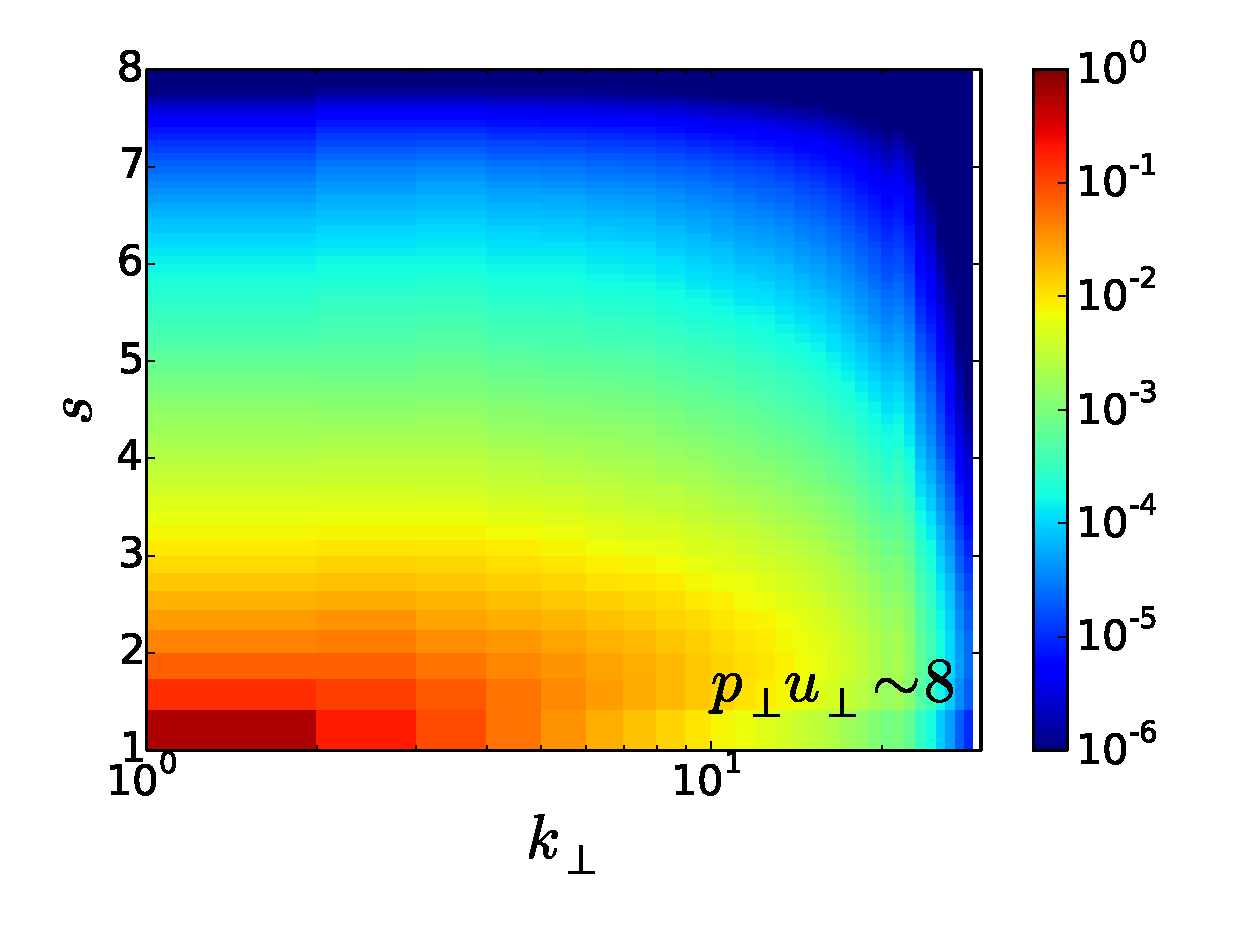
\includegraphics[width=7.4cm]{figs/phmixnlpp0/M100_8_vsskp.eps}
        \includegraphics[width=7.4cm]{figs/phmixnlpp0/M100_16_vsskp.eps}
        \caption{The spectrum $\Fsk$ vs $s-k_\perp$ at $\kpar=1$, for four different 
        $\pu$.
        For larger values of $\pu$, the spectrum does not extend far into Hermite space, as expected.}
        \label{pp0:fig:vsskp}
    \end{center}
    \end{figure}

    We observe in our simulations, that when the nonlinear timescale is faster than the linear timescale, the passive scalar
    does not get phase-mixed. This is shown in \figref{pp0:fig:vsskp}, where we see
    the spread of the spectrum in $s$ to be strongly dependent on the strength of the
    nonlinearity. \Figsand{pp0:fig:vss}{pp0:fig:fixkpvss} show this dependence---the spectrum decays exponentially in
    $s$ at a rate proportional to $\pu/k_{\parallel0}\vth$. 
    \begin{figure}
    \begin{center}
        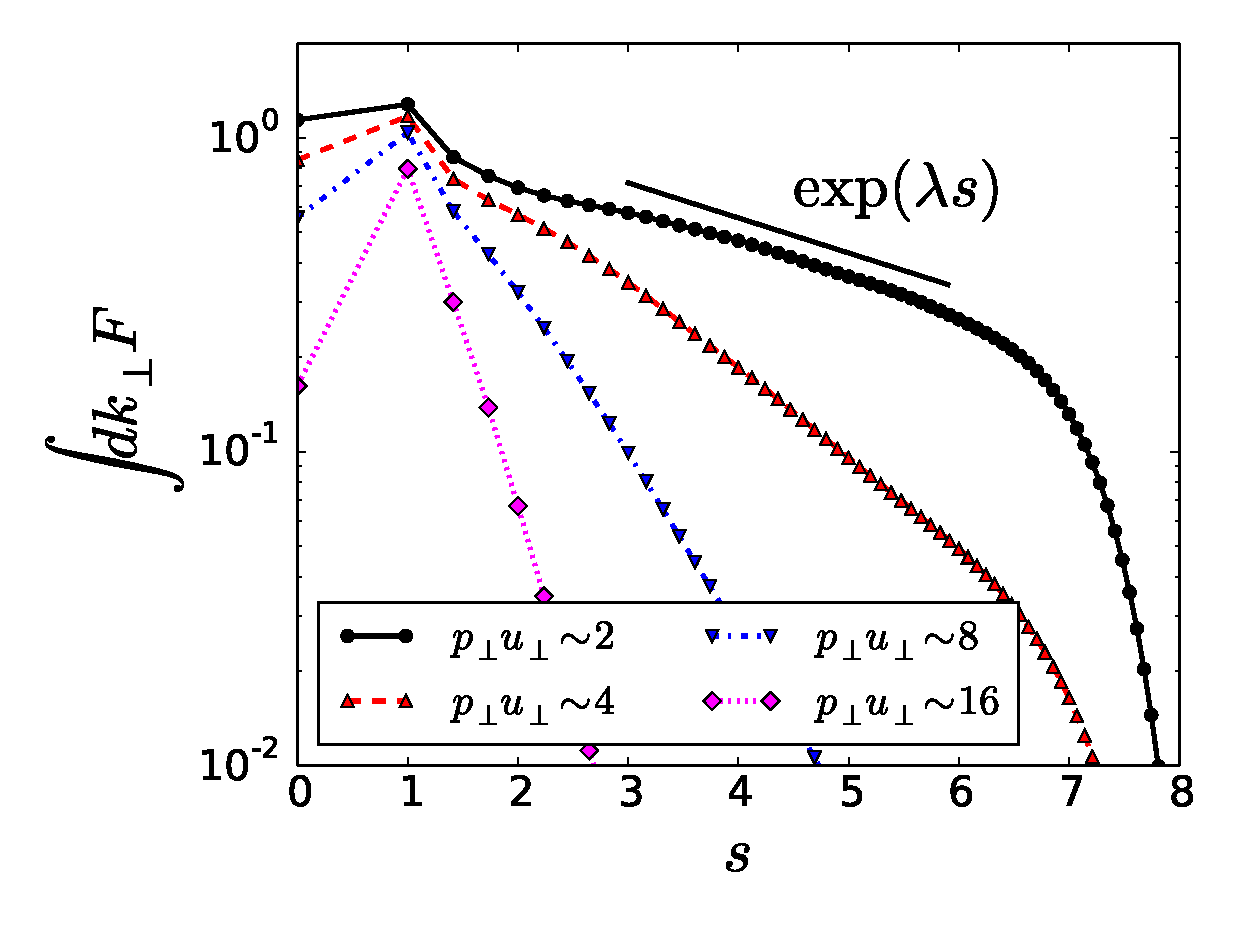
\includegraphics[width=7.4cm]{figs/phmixnlpp0/M100_vss.eps}
        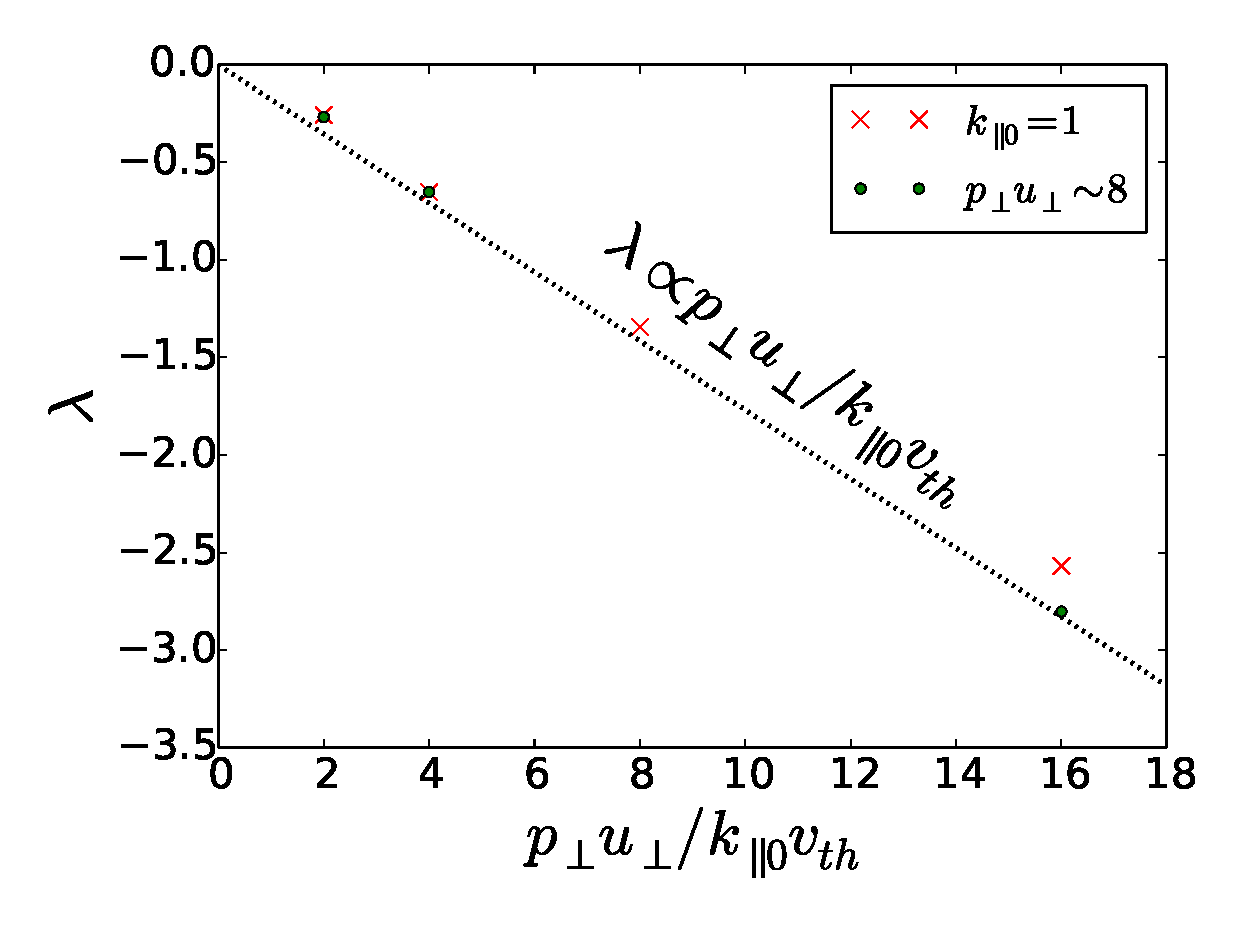
\includegraphics[width=7.4cm]{figs/phmixnlpp0/lambda_vs_gperp.eps}
        \caption{The 1D spectrum $\int dk_\perp \Fsk$ vs $s$ (left) is seen to be an exponential
        decay at a rate $\lambda$ proportional to $\pu/k_{\parallel0}\vth$. The decay rate
        is plotted versus $\pu/k_{\parallel0}\vth$ on the right---the red crosses are
        runs with fixed $k_{\parallel0}=1$ and varying $\pu$, whereas the green circles
        are runs with fixed $\pu \sim 8$ and varying $k_{\parallel0}$.}
        \label{pp0:fig:vss}
    \end{center}
    \end{figure}
    \begin{figure}
    \begin{center}
        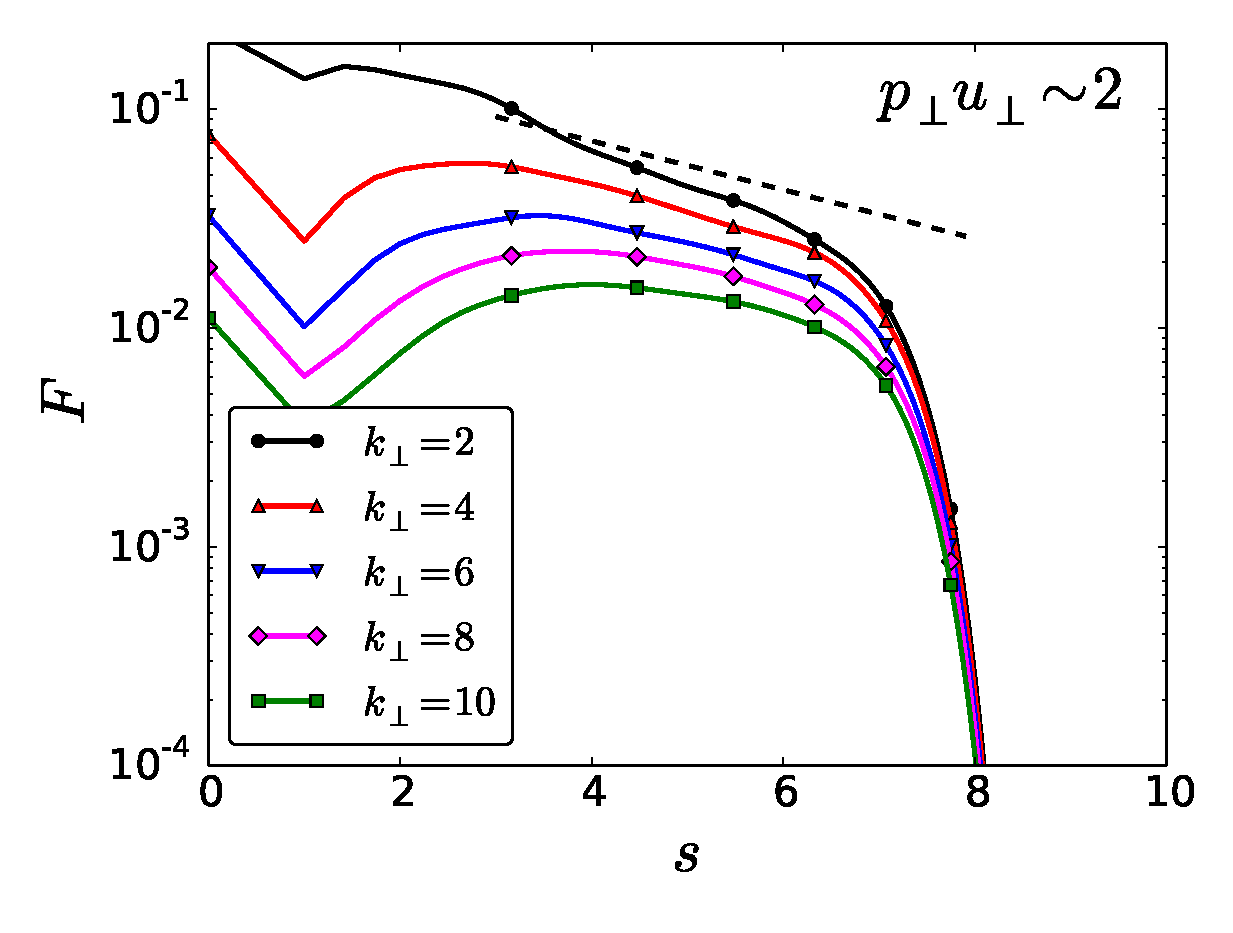
\includegraphics[width=7.4cm]{figs/phmixnlpp0/M100_2_fixkp_vss.eps}
        \includegraphics[width=7.4cm]{figs/phmixnlpp0/M100_4_fixkp_vss.eps}

        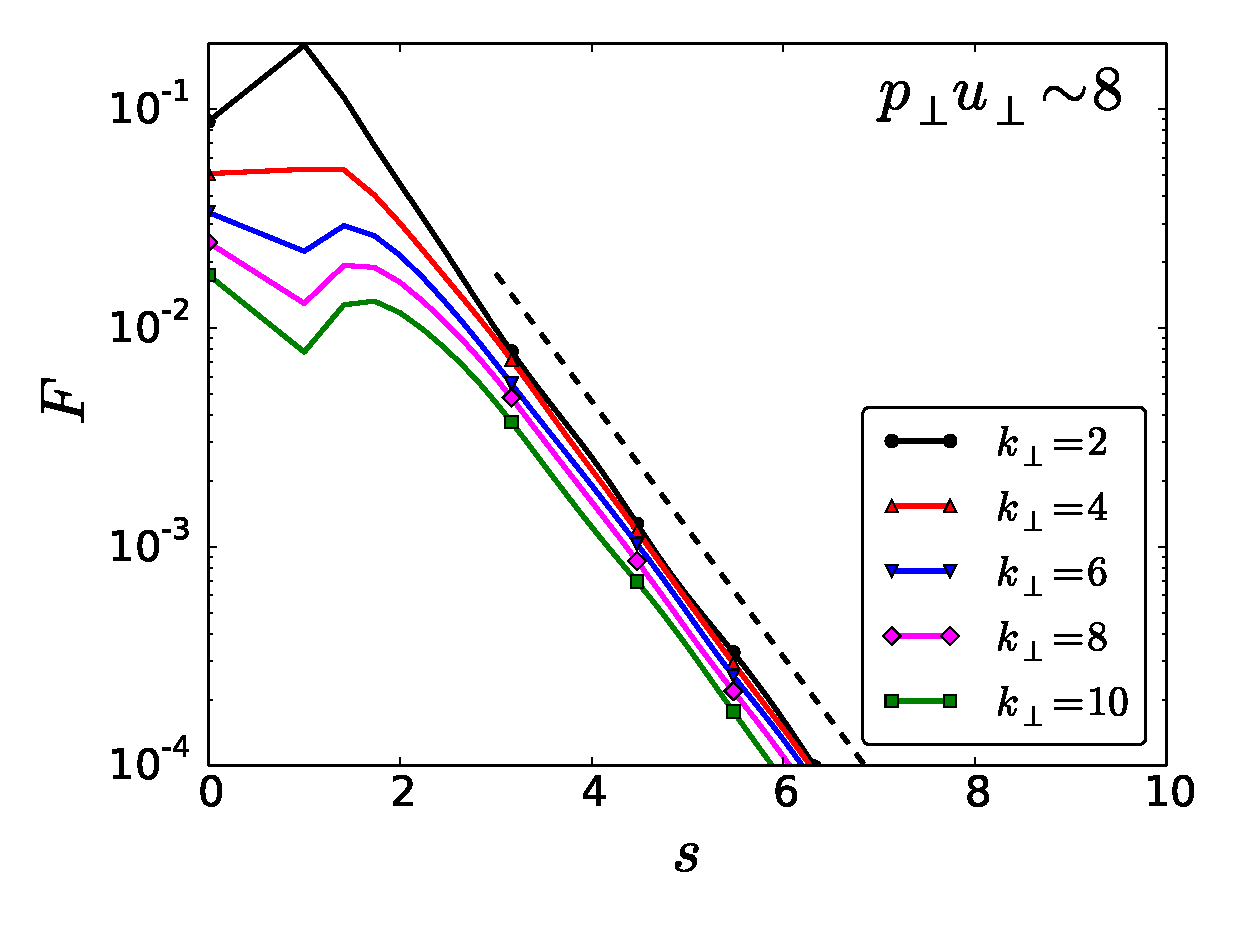
\includegraphics[width=7.4cm]{figs/phmixnlpp0/M100_8_fixkp_vss.eps}
        \includegraphics[width=7.4cm]{figs/phmixnlpp0/M100_16_fixkp_vss.eps}
        \caption{Spectrum $F$ at fixed $k_\perp$ vs $s$ for four different values of
        $\pu$.
        After an initial ``transient" in $s$, the spectrum decays exponentially at a
        rate $\propto \pu/k_{\parallel0} \vth$---the dashed line depicts the
        expected spectrum.}
        \label{pp0:fig:fixkpvss}
    \end{center}
    \end{figure}
    This is further confirmed by \figref{pp0:fig:vskp}, where the passive scalar is shown
    to have a perpendicular spectrum consistent with the fluid limit.
    \begin{figure}
    \begin{center}
        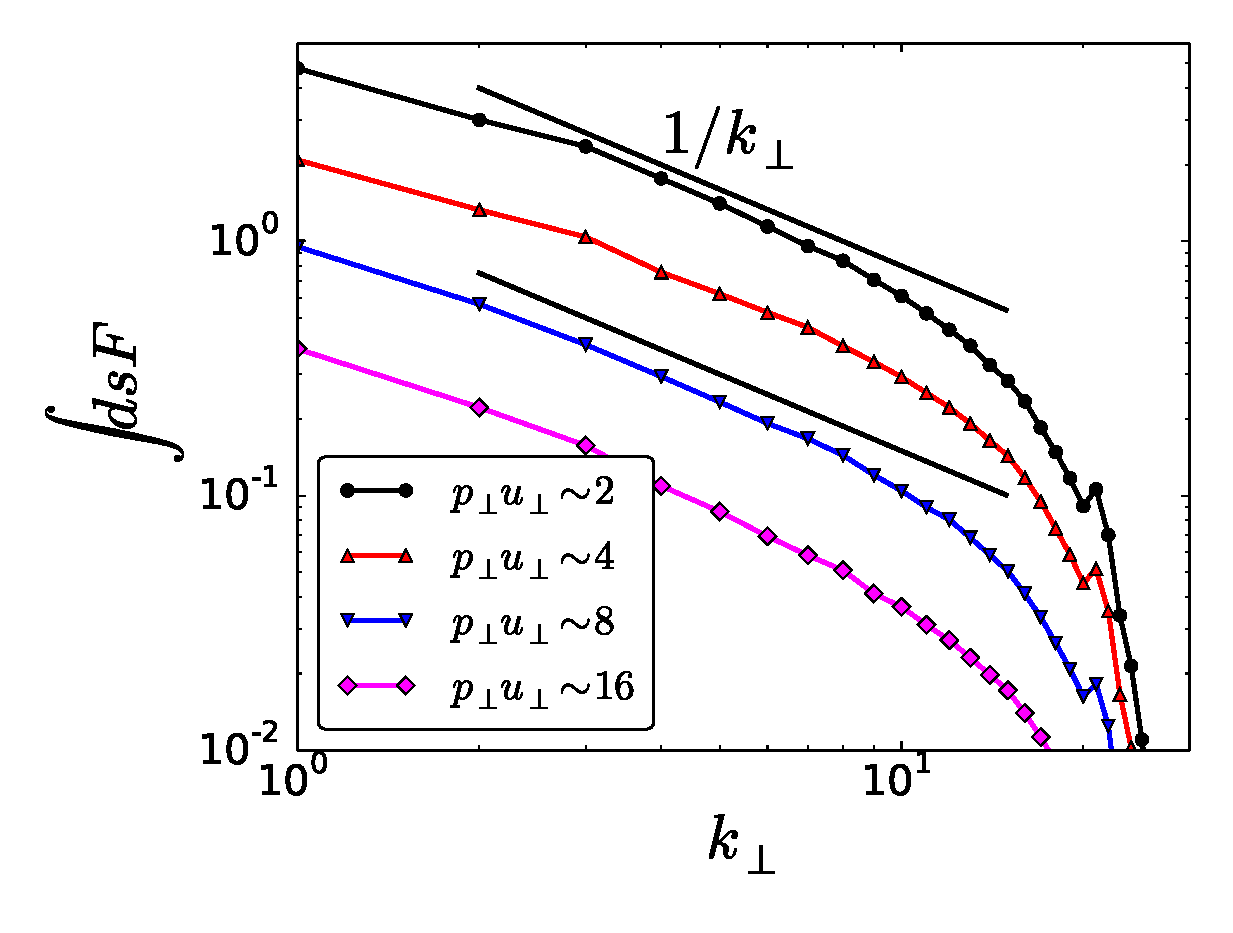
\includegraphics[width=14.8cm]{figs/phmixnlpp0/M100_vskp.eps}
        \caption{1D spectrum $\int ds \Fsk$ vs $k_\perp$. The spectrum becomes
        increasingly fluid-like ($\sim1/k_\perp$), as $\pu$ is increased.}
        \label{pp0:fig:vskp}
    \end{center}
    \end{figure}

    In \figref{pp0:fig:normcoll} we plot the dissipation due to collisions normalized to the
    total dissipation (collisional and diffusion) as a function of $\pu/k_{\parallel0}\vth$,
    where we see that the dissipation due to collisions decreases
    exponentially as the nonlinear advection rate is increased with respect to the linear
    frequency, i.e., once nonlinear, the system preferentially dissipates via diffusion.
    
    \begin{figure}
    \begin{center}
        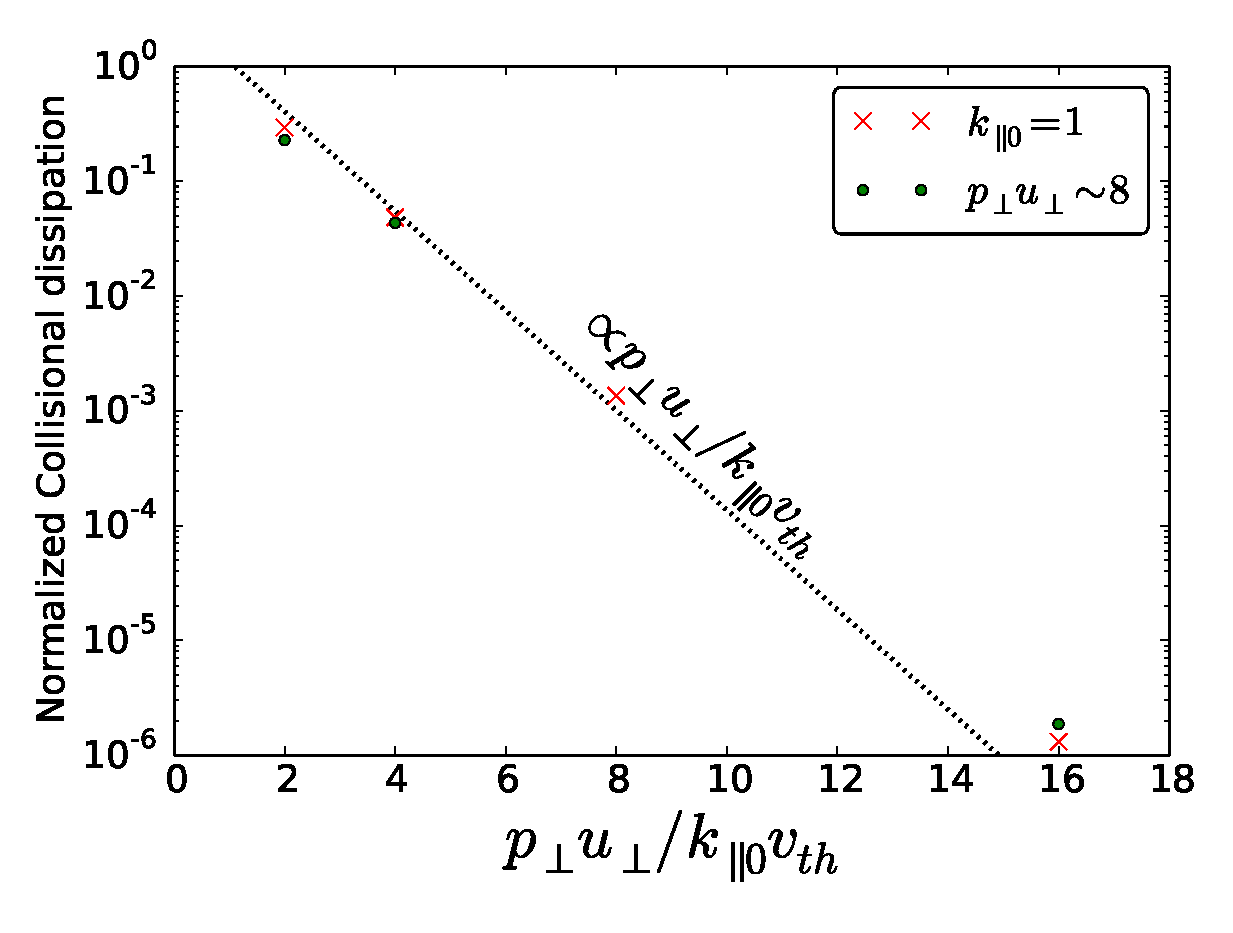
\includegraphics[width=14.8cm]{figs/phmixnlpp0/M100_normcoll.eps}
        \caption{Collisional dissipation normalized to the total dissipation vs
        $\pu/k_{\parallel0\vth}$. As the system becomes more nonlinear, most of
        the energy is dissipated by the diffusive cutoff, and vanishingly small amount of energy is dissipated
        via the collisional channel.}
        \label{pp0:fig:normcoll}
    \end{center}
    \end{figure}

\section{Discussion}
    We showed by numerically solving \eqsdash{pp0:eq:driftkin}{pp0:eq:boltz}, that if a
    kinetic passive scalar is being advected by a 2D velocity field, in the strongly
    nonlinear regime, the steady-state
    behavior is fluid-like. The nonlinear cascade
    transfers the energy to finer perpendicular
    scales, not allowing the scalar to phase mix. As a result, the perpendicular spectrum
    for such a system in the Batchelor limit is the well-known fluid spectrum:
    $1/k_\perp$. The spectrum in Hermite space decays exponentially at
    the rate $\pu/k_{\parallel0}\vth$, which is consistent with the fluid-like behavior of
    the system. 
    The dissipation for
    such a system happens almost completely through diffusion, since negligible
    amount of energy is transferred to small scales in velocity space, which makes
    collisions inaccessible.

    It has been suggested that the compressive fluctuations in the solar wind do not
    undergo a parallel cascade \cite{tome} (see \secref{slowmodes:sec:intro} for a
    detailed discussion). If this is assumed to be true, then the results presented in
    this chapter help explain the observed power law spectra of density fluctuations. In
    KRMHD, the nonlinear cascade rate associated with the background Alfv\'{e}nic
    turbulence increases with the perpendicular wavenumber; whereas, in absence of a
    parallel cascade, the linear
    phase mixing rate of the compressive fluctuations remains unchanged. As a result, beyond a certain scale the nonlinear
    cascade dominates, and disallows the slow modes to phase mix, resulting in a
    fluid-like turbulent cascade, \ie, power law spectra.
    
    The results discussed in this chapter are the kinetic generalization of the Batchelor spectrum for a 
    passive scalar, where the advecting velocity is 2D and the scalar does not undergo a
    parallel cascade. We discuss the effects of parallel cascade in the next chapter, by
    considering a 3D advecting velocity field.
    

\chapter{Kinetic passive scalar advection by 3D velocity}
\label{chap:phmixnl}
\section{Introduction}

    We saw in earlier chapters that phase mixing damps electromagnetic fluctuations and
    drives sharp velocity space gradients in the perturbed distribution function, which
    are eventually smoothed by collisions. The regularization of velocity gradients by
    collisions produces entropy and heats the plasma.
    For a linear system with a single Fourier
    mode, this is seen as a damping solution to the dispersion relation (see
    \figref{phmixlin:fig:gamma_omega}). However, the behavior of Landau
    damping in nonlinear turbulent systems, where multiple Fourier modes are coupled with
    each other is not fully understood.
    Some phenomenological models model the turbulent cascade by assuming that if the linear
    damping rate is comparable to, or larger than the nonlinear cascade rate
    scale-by-scale, a part of the energy is pumped into small velocity space scales at
    each spatial scale \cite{quataert98, quataert99, howes08jgr}. This, in essence,
    superimposes the linear damping physics on to the nonlinear turbulent cascade.
    However, such scale-by-scale extraction of energy results in an exponentially decaying energy spectrum \cite{gary09,
    podesta10}, which is not seen in numerical simulations \cite{howes08prl,
    barnes11, tenbarge12} or in observations \cite{celnikier83, celnikier87, coles89,
    marsch90, coles91, bershadskii04, hnat05, kellogg05,
    chen11, sahraoui09, alexandrova09, chen10, sahraoui10, alexandrova12, sahraoui13,
    chen13}. Understanding how Landau damping (or, more generally, phase mixing) operates
    in a turbulent environment is essential in addressing this discrepancy.

    \begin{figure}
    \begin{center}
        \includegraphics[width=14.8cm]{figs/phmixnl/uperp_3D.png}
        \caption{The velocity field $\mathbf{u}_\perp$ vs $x$ and $y$ for different values
        of $z$.}
        \label{phmixnl:fig:uperp}
    \end{center}
    \end{figure}
    
    In \chapref{chap:pp0}, we approached this problem by considering a model for a passive
    kinetic scalar being advected by a 2D chaotic velocity. There, the phase mixing rate
    for the scalar was fixed by its initial wavenumber. Therefore, for strongly
    nonlinear systems, the scalar spectrum with respect to $s$ was a sharp exponential
    decay. 
    In
    this chapter, we extend the analysis from \chapref{chap:pp0} to a 3D advecting
    velocity field (see \figref{phmixnl:fig:uperp}). Due to the 3D structure of the velocity, the scalar now undergoes a
    parallel cascade in addition to the perpendicular one. Hence, unlike the 2D velocity
    case, the scalar now has access to larger $\kpar$, and may phase mix more efficiently.
    Interestingly, we do not observe increased phase mixing efficiency in our numerical
    simulations.
    Instead, we see that the energy gets scattered in the phase space in such a
    way, that it generates a significant
    amount of return flux of energy from small to large velocity scales. We identify this
    effect as the stochastic analog of the plasma echo in
    a turbulent system. As a result, the net flux
    to small velocity scales is suppressed, effectively reducing the phase mixing
    efficiency. Suppression of phase mixing by the turbulent plasma echo
    helps explain the power law energy spectra at kinetic scales in turbulent
    plasmas, even when the scalar has a parallel cascade\footnote{The case of no parallel
    cascade was discussed in \chapref{chap:pp0}, where it was shown that in the nonlinear
    limit energy in the scalar is swept up to small spatial scales before it can phase
    mix---resulting in power law spectra.}. 

\section{Kinetic model}
    We consider a homogeneous magnetized plasma close to a Maxwellian equilibrium threaded by
    a background magnetic field $\mb{B_0} = B_0 \hat{\mb{z}}$; with all fluctuations
    low-frequency compared to the cyclotron frequency. We assume that it suffices to describe
    only one particle species (ions or electrons) kinetically, and calculate the evolution of the
    other species using an appropriate Boltzmann response. We further assume 
    all wavelengths to be large compared to the kinetic species' Larmor radius. Such a
    system is described using a (3+1)D model,
    with three spatial co-ordinates $x, y, z$ and one velocity co-ordinate $\vpar$ parallel to the
    background magnetic field; the remaining velocity co-ordinates are integrated out.
    The perturbed distribution function $g$ of the kinetic species satisfies a 
    ``drift-kinetic" equation\footnote{This equation could have also been derived from KRMHD
    in the same way as \chapref{chap:pp0}. By giving an alternate presentation here, we
    emphasize the general applicability of this equation beyond KRMHD.}:
\beq
     \partial_t g + \mathbf{u}_\perp \cdot \nabla_\perp g + \vpar \nabla_\parallel
     (g + \phi F_0) = C[g] + \eta \nabla_\perp^2 g + \chi, \label{phmixnl:eq:driftkin}
   \eeq
   \beq
     \phi  = \alpha \int_{-\infty}^\infty d \vpar g(\vpar).  \label{phmixnl:eq:boltz}
   \eeq
   Here $\mathbf{u}_\perp$ is a ``fluid" drift velocity that mixes the perturbed
   distribution function perpendicular to the magnetic field, $\vpar
   \nabla_\parallel g$ is the parallel streaming term that phase-mixes the distribution
   function, i.e. generates $\vpar$ structure, $C[g]$ is a
   collision operator (diffusive in $\vpar$) that smooths this structure in an
   irreversible manner,
   $\eta \nabla_\perp^2 g$ is a diffusive term that extracts energy from the system
   at small perpendicular scales (and stands in for a possibly more complicated cutoff
   associated with finite-Larmor-radius physics). The equilibrium distribution function
   $F_0~=~e^{-\vpar^2/\vth^2}/\sqrt{\pi} \vth$ is a Maxwellian, where
   $\vth=\sqrt{2 T/m}$, $T$ is the temperature and $m$ the mass of
   the reference species, and the equilibrium density is assumed to be unity. $-\nabla_\parallel \phi$ is the normalized (by the parameter
   $\alpha$) parallel electric field, and $\chi$ is a source that injects energy into the
   system.

   
   \Eqsdash{phmixnl:eq:driftkin}{phmixnl:eq:boltz} describe qualitatively or, in some cases,
   quantitatively, a multitude of plasmas, for \textit{e.g.} ion-acoustic perturbations
   in a proton-electron plasma, in which case $\alpha = T_e/T_i$ ($T_e$ and $T_i$ are temperatures
   of electrons and ions respectively) and $\mb{u_\perp} = v_{thi}
   \hat{z}\times \rho_i \nabla \phi/2$ ($\rho_i$ is the ion Larmor radius) is the
   $\EcrossB$ drift velocity. In this electrostatic system, the fluctuating electric field,
   and hence the drift velocity, is set by the density fluctuations of the perturbed distribution function $g$. In contrast,
   compressive fluctuations in electromagnetic plasmas decouple from the Alfv\'{e}nic
   turbulence in the long wavelength limit, and are
   passively advected by the velocity fluctuations due to the Alfv\'{e}nic
   turbulence \cite{tome}. For such a system, the velocity $\mb{u_\perp}$ is independent of the perturbed distribution function $g$; the
   parameter $\alpha$ depends on plasma beta, $T_i/T_e$ and the ion charge\footnote{See
   eqs.~181 and 182 of Schekochihin et al. \cite{tome}, $\alpha$ is related to their
   $\Lambda$ as $\alpha=-1/\Lambda$.}. 
   
\subsection{Hermite space dynamics}
\label{sec:hermite}

    The linear Hermite space formalism developed in \secref{phmixlin:sec:Hermite} can be
    generalized to the nonlinear model at hand as follows. \Eqref{phmixnl:eq:boltz} becomes
\beq
    \phi = \alpha g_0,
    \label{phmixnl:eq:boltz_g0}
\eeq
whereas the kinetic equation (\eqref{phmixnl:eq:driftkin}) turns into a set of fluid-like
equations (similar to \eqsdash{phmixlin:eq:g0}{phmixlin:eq:gmeq})
in which phase mixing is manifested as a coupling between neighboring Hermite moments:
\begin{align}
    \label{phmixnl:eq:g0}
    &\od{g_0}{t} + \vth \nabla_\parallel\frac{g_1}{\sqrt{2}}  = \eta \nabla_\perp^2
    g_0 + \chi_0,\\
    \label{phmixnl:eq:g1}
    &\od{g_1}{t} + \vth \nabla_\parallel\lt(g_2 + \frac{1+\alpha}{\sqrt{2}}\,g_0\rt)
    = \eta \nabla_\perp^2 g_1 + \chi_1,\\
    &\od{g_m}{t} + \vth \nabla_\parallel\lt(\sqrt{\frac{m+1}{2}}\,g_{m+1} +
    \sqrt{\frac{m}{2}}\,g_{m-1}\rt) \nonumber \\
    &= -\nu m g_m + \eta \nabla_\perp^2 g_m,  \quad m\ge2.
    \label{phmixnl:eq:gmeq}
\end{align}
Here $d/dt = \lt(\partial_t + \mb{u_\perp}\cdot \nabla\rt)$ is the convective derivative, 
$-\nu m g_m$ is the Hermite transform of the Lenard-Bernstein collision operator
\cite{lenard58}, and $\nu$ is the collision
frequency. Energy is injected into the system by driving
$g_0$ and/or $g_1$ using the source terms $\chi_0$ and $\chi_1$. The energy then propagates to higher $m$. 
We will later
see that a perturbation at high $m$ can be coupled back to low $m$ through the
nonlinear interaction---this is the ``phase-unmixing" component, the stochastic
turbulent analog of the plasma echo.

Upon Fourier transforming \eqref{phmixnl:eq:gmeq} in space, $(x, y, z) \to \mb{k}$ and
defining $\tgmk =
\lt(i \sgn \kpar\rt)^m \gmk$, where $\kpar$ is the component of $\mb{k}$ parallel to
$\mb{B}_0$, one finds
\bea
    \pd{\tgmk}{t} + \frac{|\kpar| \vth}{\sqrt{2}} \lt(\sqrt{m+1} \tg_{m+1,\mb{k}} -
    \sqrt{m} \tg_{m-1, \mb{k}} \rt) = \nonumber \\
    \sum_{\mb{p}, \mb{q}} \Mkpq \lt[\sgn\lt(\kpar
    q_\parallel\rt)\rt]^m \Phip \tgmq 
    - \nu m \tgmk \nonumber \\- \eta k_\perp^2 \tgmk, \label{phmixnl:eq:tgmk}
\eea
where $\Phi$ is the stream function for the drift velocity, $\mb{u_\perp} =
\hat{\mb{z}}\times \nabla \Phi$ and $\Mkpq = - \hat{z} \cdot (\mb{p} \times \mb{q})\, \delta_{\mb{k},\mb{p+q}}$.

If we assume weak collisions $\nu \ll |\kpar| \vth$, large values of $m$,
$1\ll~m~\ll~(|\kpar|\vth/\nu)^2$, remain undamped. 
For such large $m$, the second term on the left hand side of \eqref{phmixnl:eq:tgmk} is dominant. This implies $\tg_{m+1} \approx
\tg_{m-1}$, i.e., $\tg_{m+1} \approx \pm \tgm$. Hence, there are two solutions: one
where $\tgm$ is continuous, and the other where $(-1)^m \tgm$ is. Thus $\tgm^+ =
(\tgm+\tg_{m+1})/2$ and $\tgm^-=(-1)^m(\tgm - \tg_{m+1})/2$ are both continuous in $m$
(see also \secref{phmixlin:sec:cont})\footnote{Note that the $``+"$ and $``-"$ fields here are not
the same as the ones in \eqref{intro:krmhd:gpm}.}.
We would like to approximate the second term on the left hand side of \eqref{phmixnl:eq:tgmk} as a
derivative in $m$. Since $\tgmk^\pm$ are continuous in $m$, we can derive 
approximate evolution equations\footnote{Except
for the nonlinear terms on the right hand side, this is the same equation as
\eqref{phmixlin:eq:gpmevol}.} (valid to $O(1/\sqrt{m})$) for $\tgmk^\pm$ from
\eqref{phmixnl:eq:tgmk}, by expanding in the small parameter $1/\sqrt{m}$
\begin{align}
    &\pd {\tgmk^\pm}{t} \pm \sqrt{2} |k_\parallel| \vth m^{1/4} \pd{}{m} m^{1/4}
    \tgmk^\pm +
    \nu m \tgmk^\pm \nonumber \\
    & = \sum_{\mb{p},\mb{q}} M_{\mb{kpq}}
     \Phi_\mb{p} \lt(\delta_{k_\parallel, q_\parallel}^+ \tgmq^\pm +
     \delta_{k_\parallel, q_\parallel}^- \tgmq^\mp \rt) 
     - \eta k_\perp^2 \tgmk^\pm, \label{phmixnl:eq:gpm}
\end{align}
where $\delta_{\kpar,\qpar}^\pm = 1$ if $\kpar$ and $\qpar$ have the same/opposite
sign and 0 otherwise (the sign of $\kpar=0$ is taken to be positive).
%
%We make a further simplifying assumption that the drift velocity
%$\mb{u}_\perp = \hat{\mb{z}}\times\Phi$ is independent of the perturbed distribution function $g$. We model the
%velocity field using a Langevin equation:
%\beq
%\pdt
%    \Phi + \gamma \Phi = \kappa, \quad \la \kappa(t) \kappa(t') \ra = \epsilon
%    \delta(t-t'), 
%\eeq
%where $\gamma>0$ and $\kappa$  is a Gaussian white noise source term which drives $\Phi$
%with power $\epsilon$. The velocity is also assumed to be single scale, which is taken to
%be the largest scale in the system.
%
%\begin{figure}
%\begin{center}
%    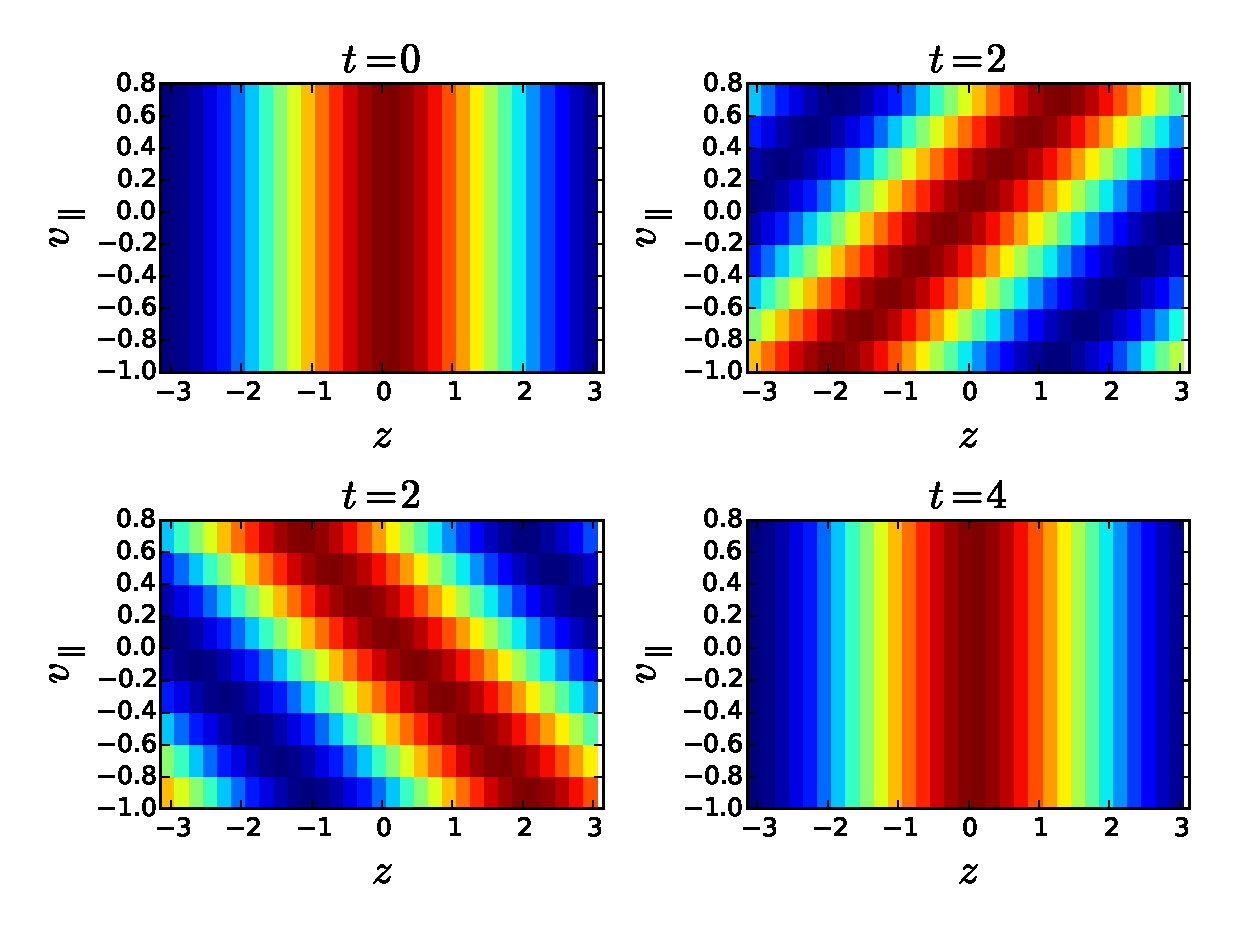
\includegraphics[width=14.8cm]{figs/phmixnl/echo_cartoon.eps}
%    \caption{A cartoon sketch showing how a phase-mixing mode is converted to an
%    phase-unmixing mode. The top left plot shows a phase-mixing mode in the $(z,\vpar)$
%    plane, at time $t=0$ (in
%    arbitrary units) with some parallel structure and no structure in velocity space; this
%    mode then phase-mixes to the one shown in the top right plot at time $t=2$; at which
%    point }
%    \label{phmixnl:fig:echocartoon}
%\end{center}
%\end{figure}
%
There are three separate physical effects manifest in \eqref{phmixnl:eq:gpm}: 
\begin{inparaenum}[(i)]
\item phase mixing/unmixing---the left hand side of \eqref{phmixnl:eq:gpm} is an advection equation in $m$, where
$``+"$ (phase-mixing) modes propagate from small $m$ to large,
and $``-"$ (phase-unmixing) modes propagate from large $m$ back to small; 
\item turbulent cascade---the first term on the right hand side describes nonlinear
coupling of modes with different wavenumbers, which generates fluctuations at small spatial scales;
\item plasma echo---the second term on the right hand side couples the phase-mixing and
phase-unmixing components via nonlinear interaction with the drift velocity. This allows
for a phase-mixing mode propagating to large $m$ to be converted to an phase-unmixing
mode which would propagate back to small $m$, and vice versa.
\end{inparaenum}

In the absence of nonlinear advection ($\Phi = 0$), there is no turbulent cascade, and the
phase-mixing and phase-unmixing
components are decoupled. In this ``linear" limit it can be proven analytically that $\tgm^- = 0$ to lowest
order in $1/\sqrt{m}$, i.e., there is no plasma echo (see \cite{kanekar14a},
\chapref{chap:phmixlin}). Another instance where a
complete lack of an echo can be shown, is when the drift velocity is 2D
($\ppar=0$). Then, the resonance condition $\kpar = \qpar + \ppar = \qpar$ does not allow
$\kpar$ and $\qpar$ to have opposite signs, which according to \eqref{phmixnl:eq:gpm} is a necessary
condition for coupling between phase-mixing and phase-unmixing modes.
Unlike the linear or the 2D drift velocity limit,
a 3D drift velocity ($\ppar\neq0$) has all three aforementioned effects existing
simultaneously in the system.

\subsection{Energetics}
\label{phmixnl:sec:energetics}

In order to understand the relative importance of these three effects, we diagnose how the
free energy of perturbations, $W = \int d
\mb{r} \lt(\int d \vpar \langle g^2 \rangle/2 F_0 + \langle \phi^2 \rangle/2 \alpha
\rt)=\int~d\mb{r}\lt[~\sum_m~|g_m|^2+|g_0|^2~(1+\alpha)\rt]$ gets distributed in the phase
space by the dynamics of the system. $W$ is conserved by \eqsdash{phmixnl:eq:driftkin}{phmixnl:eq:boltz}
in absence of dissipation (see Refs.~\cite{schekochihin08, tome, kanekar14a} and
\secref{intro:sec:krmhd:const}).
Phase mixing transfers $W$ from small $m$ to large, phase unmixing brings it back from
large
$m$ to small. Nonlinear advection cascades $W$ to small spatial scales. 

The contribution of individual Hermite moments to the total free energy $W$, 
is given by
$\Fsk=\sqrt{m}k_\perp~|\tgmk|^2$, where we have changed the Hermite space variable
from $m$ to $s=\sqrt{m}$. At large $s$, $\Fsk$ can be split into the phase-mixing ($\Fsk^+$) and
phase-unmixing components ($\Fsk^-$), where $\Fsk^\pm=\sqrt{m}k_\perp~|\tgmk^\pm|^2$ (see
\eqref{phmixnl:eq:gpm}).
To derive evolution equations for
$\Fsk^\pm$, multiply \eqref{phmixnl:eq:gpm} by
$\sqrt{m}~k_\perp~\tgmk^{\pm \star}$ (the asterisk denotes complex conjugate), to
obtain
\bea
    \pd{\Fsk^\pm}{t} \pm \frac{\lt|\kpar\rt|\vth}{\sqrt{2}} \pd{\Fsk^\pm}{s} + 2 \nu
    s^2 \Fsk^\pm + 2 \eta k_\perp^2 \Fsk^\pm =  
    \textit{Nonlinear terms}.
    \label{phmixnl:eq:Fskpm}
\eea
We can now define the flux of energy from low to high $s$ in the large $s$ limit: 
$\Gsk = \lt|\kpar\rt| \vth \lt(\Fsk^+-\Fsk^-\rt)/\sqrt{2}$. The efficiency of phase mixing is then given by the
normalized flux $\sqrt{2}\Gsk/
|\kpar|\vth\Fsk = (\Fsk^+ - \Fsk^-)/(\Fsk^+ + \Fsk^-)$---phase mixing is completely suppressed when this quantity
is zero, whereas when it is one, the amount of phase mixing is same as that for the linear
system. 
An exact expression for the
flux that is valid at all $s$  can be calculated directly from 
\eqref{phmixnl:eq:tgmk}: $\Gsk~=~\lt|\kpar\rt| \vth \sqrt{(m+1)/2} \, \Re \langle
\tg_{m+1,\mb{k}} \tgmk^\star \rangle$. %

\section{Numerical setup}
    
    We solve \eqsdash{phmixnl:eq:g0}{phmixnl:eq:gmeq} numerically using \Gand.
%    a pseudo-spectral
%    scheme: Hermite moments of the perturbed distribution function are represented using
%    Fourier modes, the nonlinear term is calculated in real space. 
%    Due
%    to the background magnetic field, the system described by \eqsdash{phmixnl:eq:driftkin}{phmixnl:eq:boltz}
%    is anisotropic: the parallel wavelengths of all fluctuations are much longer compared
%    to the perpendicular wavelengths. To facilitate an efficient numerical implementation
%    we normalize the perpendicular spatial co-ordinates $x, y$ and the parallel spatial
%    co-ordinate $z$, to independent arbitrary length scales $\rho$ and $L$, respectively
%    (with the assumption $L \gg \rho$). The drift velocity
%    $\mb{u_\perp}$ is normalized to the thermal velocity $\vth$, time is normalized to
%    $L/\vth$. The Hermite moments of the distribution function are in arbitrary units.
%    The distribution function moments $g_m$ and the electric potential
%    $\phi$ are scaled up by a factor of $L/\rho$ so that all normalized terms are order unity. 
%    %Henceforth, all the quantities quoted in this paper are
    %in these normalized units.
    To simplify the analysis we assume that the distribution function is passive, i.e.,
    the drift velocity $\mb{u_\perp}$ is independent of $g$.
    The velocity $\mb{u}_\perp=\hat{\mb{z}}\times\nabla\Phi$ is
    calculated by solving the Langevin equation $\pdt
    \Phi + \gamma \Phi = \kappa$, where $\gamma >0$ and $\kappa$ is Gaussian white noise ($\langle \kappa(t) \kappa(t')\rangle =
    \epsilon \delta(t-t')$) which drives $\Phi$ with power $\epsilon$; $\gamma$ is chosen
    such that the Kubo number is held constant at one (see \secref{pp0:sec:intro}). The drift velocity
    was restricted to a single scale (all wavenumbers $\mb{p}$ such that $p_\perp=1,
    \ppar=1$), the largest scale in our numerical box.
    The
    saturated root mean square amplitude of the drift velocity can be calculated using the
    fluctuation-dissipation theorem \cite{kubo66}: $\langle u_\perp^2 \rangle
    = p_\perp^2 \epsilon/2 \gamma$. In light of these simplifications, one can estimate
    the turbulent cascade rate as $\tau_C^{-1}\sim \pu$, which we control in our simulations by
    changing $\epsilon$.
    
    The source term in \eqref{phmixnl:eq:g0}, $\chi_0$, is assumed to be delta-correlated
    in time, and
    $\chi_1$ is set to zero. Since \eqref{phmixnl:eq:driftkin} is
    homogeneous in $g$, the power with which $\chi_0$ injects energy into the system can
    be set to unity without loss of generality.

    Instead of using the Lenard-Bernstein collision operator or
    regular viscosity as in \eqref{phmixnl:eq:gmeq}, we use hypercollisions ($-\nu m^8 g_m$)
    and hyperviscosity ($-\eta k_\perp^8 g_m$) to efficiently utilize
    computational resources. The dissipation microscales for these operators can be estimated
    as $s_c = \sqrt{m_c} = \lt(\ppar \vth/\nu\rt)^{1/17}$ and $k_{\perp, \eta} = \lt(
    |u_\perp|/\eta \rt)^{1/8}$, where $s_c$ is the collisional cutoff for modes with
    parallel wavenumber $\ppar$; $k_{\perp,
    \eta}$ is the viscous cutoff. A simulation is fully characterized by 3 parameters:
    the nonlinear advection rate $\tau_C^{-1}$, the collisional cutoff $s_c$ and the viscous
    cutoff $k_{\perp, \eta}$.  
    All the results included in this chapter are from a simulation with parameters $\tau_C
    \simeq 1.5$, $s_c \simeq 21.3$ and $k_{\perp, \eta} \simeq 18.8$.

\section{Results}
    \subsection{Phase mixing efficiency}

    \begin{figure}
    \begin{center}
        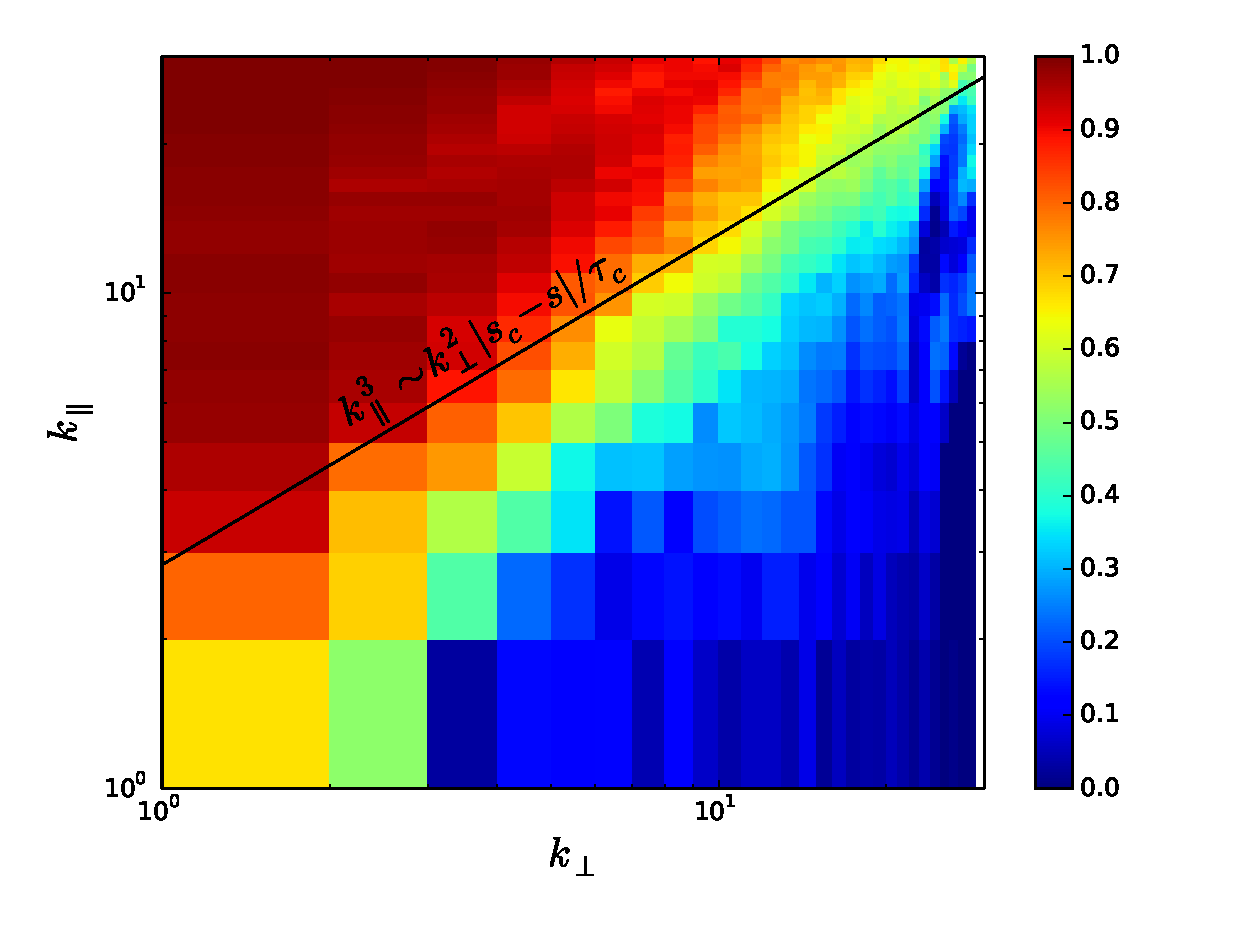
\includegraphics[width=14.8cm]{figs/phmixnl/M900_m100_pmsupp_vskpkz.eps}
        \caption{Normalized flux (defined after \eqref{phmixnl:eq:Fskpm}) through $s=10$ vs
        $k_\perp-\kpar$. Phase mixing is nearly completely suppressed for $\kpar^3 \leq
        k_\perp^2 \lt|s_c -s\rt|/\tau_C$.}
        \label{phmixnl:fig:m100supp:vskpkz}
    \end{center}
    \end{figure}
    \begin{figure}
    \begin{center}
        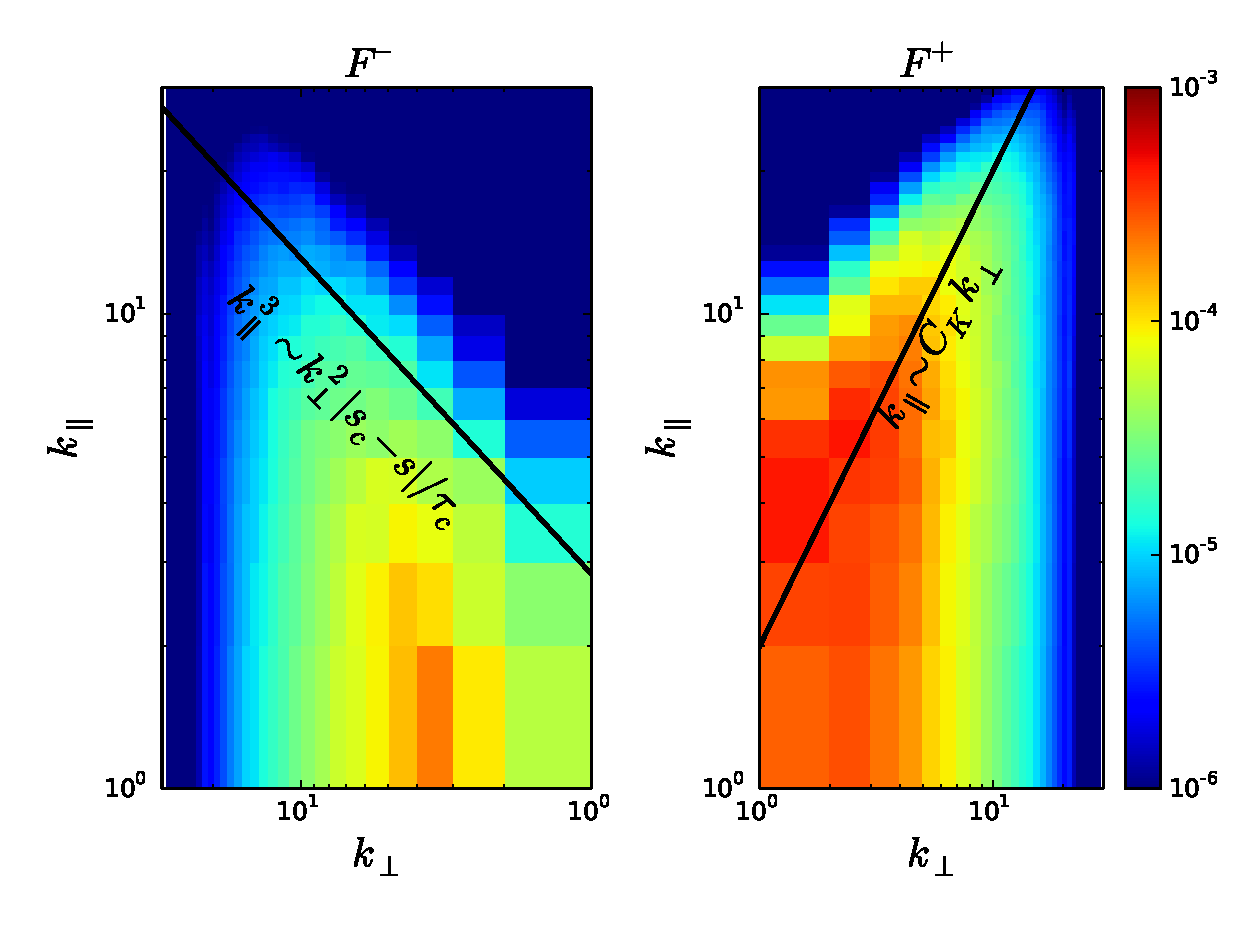
\includegraphics[width=14.8cm]{figs/phmixnl/M900_m100_fpm_vskpkz.eps}
        \caption{$\Fsk^\pm$ (defined before \eqref{phmixnl:eq:gpm}) at $s=10$ vs
        $k_\perp-\kpar$; $F^-$ is plotted on the left, $F^+$ on the right. The horizontal
        axis for $F^-$ is reversed, so as to facilitate comparison with the $F^+$
        plot. For $\kpar^3 \geq k_\perp^2 \lt|s_c-s\rt|/\tau_C$,
        there is negligible $\Fsk^-$. $\Fsk^+$ is seen to cascade to large wavenumbers
        along the $\kpar\sim C_K k_\perp$ line.}
        \label{phmixnl:fig:m100fpm:vskpkz}
    \end{center}
    \end{figure}

    \begin{figure}
    \begin{center}
        \includegraphics[width=14.8cm]{figs/phmixnl/M900_m100_pmsupp_vsskz.eps}
        \caption{Normalized flux (defined after \eqref{phmixnl:eq:Fskpm}) at $k_\perp=8$ vs
        $\kpar-s$. Phase mixing is nearly completely suppressed for $\kpar^3 \leq
        k_\perp^2 \lt|s_c -s\rt|/\tau_C$.}
        \label{phmixnl:fig:m100supp:vsskz}
    \end{center}
    \end{figure}
    \begin{figure}
    \begin{center}
        \includegraphics[width=14.8cm]{figs/phmixnl/M900_m100_fpm_vsskz.eps}
        \caption{$\Fsk^\pm$ (defined before \eqref{phmixnl:eq:gpm}) at $k_\perp=8$ vs
        $\kpar-s$; $F^-$ is plotted on the left, $F^+$ on the right. The horizontal
        axis for $F^-$ is reversed, so as to facilitate comparison with the $F^+$
        plot. For $\kpar^3 \geq k_\perp^2 \lt|s_c-s\rt|/\tau_C$,
        there is negligible $\Fsk^-$.}
        \label{phmixnl:fig:m100fpm:vsskz}
    \end{center}
    \end{figure}

    \begin{figure}
    \begin{center}
        \includegraphics[width=14.8cm]{figs/phmixnl/M900_m100_pmsupp_vsskp.eps}
        \caption{Normalized flux (defined after \eqref{phmixnl:eq:Fskpm}) at $\kpar=8$ vs
        $k_\perp-s$. Phase mixing is nearly completely suppressed for $\kpar^3 \leq
        k_\perp^2 \lt|s_c -s\rt|/\tau_C$.}
        \label{phmixnl:fig:m100supp:vsskp}
    \end{center}
    \end{figure}
    \begin{figure}
    \begin{center}
        \includegraphics[width=14.8cm]{figs/phmixnl/M900_m100_fpm_vsskp.eps}
        \caption{$\Fsk^\pm$ (defined before \eqref{phmixnl:eq:gpm}) at $\kpar=8$ vs
        $k_\perp-s$; $F^-$ is plotted on the left, $F^+$ on the right. The horizontal
        axis for $F^-$ is reversed, so as to facilitate comparison with the $F^+$
        plot. For $\kpar^3 \geq k_\perp^2 \lt|s_c-s\rt|/\tau_C$,
        there is negligible $\Fsk^-$.}
        \label{phmixnl:fig:m100fpm:vsskp}
    \end{center}
    \end{figure}

    Since we chose the drift velocity to be a single scale velocity field with $\ppar=1$,
    the nonlinear term couples modes whose parallel wavenumbers differ from each other by
    one. A phase mixing mode at $s=1$, with a parallel wavenumber $\kpar$, is converted to
    an phase-unmixing mode only if the two have oppositely signed parallel wavenumbers
    (see \eqref{phmixnl:eq:gpm}). Hence, such a phase-mixing mode has to go through at least
    $\kpar$ nonlinear interactions in order to reach $\kpar=0$, before it can be
    converted to an phase-unmixing mode.
    While this phase-mixing mode cascades to
    $\kpar=0$, it also gets transferred to a larger $s$ due to phase mixing. If this value
    of $s$
    is comparable to the collisional cutoff $s_c$, a part of the energy is lost to
    collisions, and only the remaining energy gets converted to an phase-unmixing mode---this sets a bound on the extent of the plasma echo in the phase space. 
    We observe in our simulations that the plasma echo is restricted to the $\kpar^3 \leq
    k_\perp^2 \lt|s_c-s\rt|/\tau_C$ region of the phase space as seen in
    \figsdash{phmixnl:fig:m100supp:vskpkz}{phmixnl:fig:m100fpm:vsskp}.
    As a result of the echo, phase mixing is significantly suppressed for $\kpar^3~\leq~k_\perp^2 \lt|s_c-s\rt|/\tau_C$. 

\subsection{Spectra vs $(s, k_\perp, \kpar)$}

    \begin{figure}
    \begin{center}
        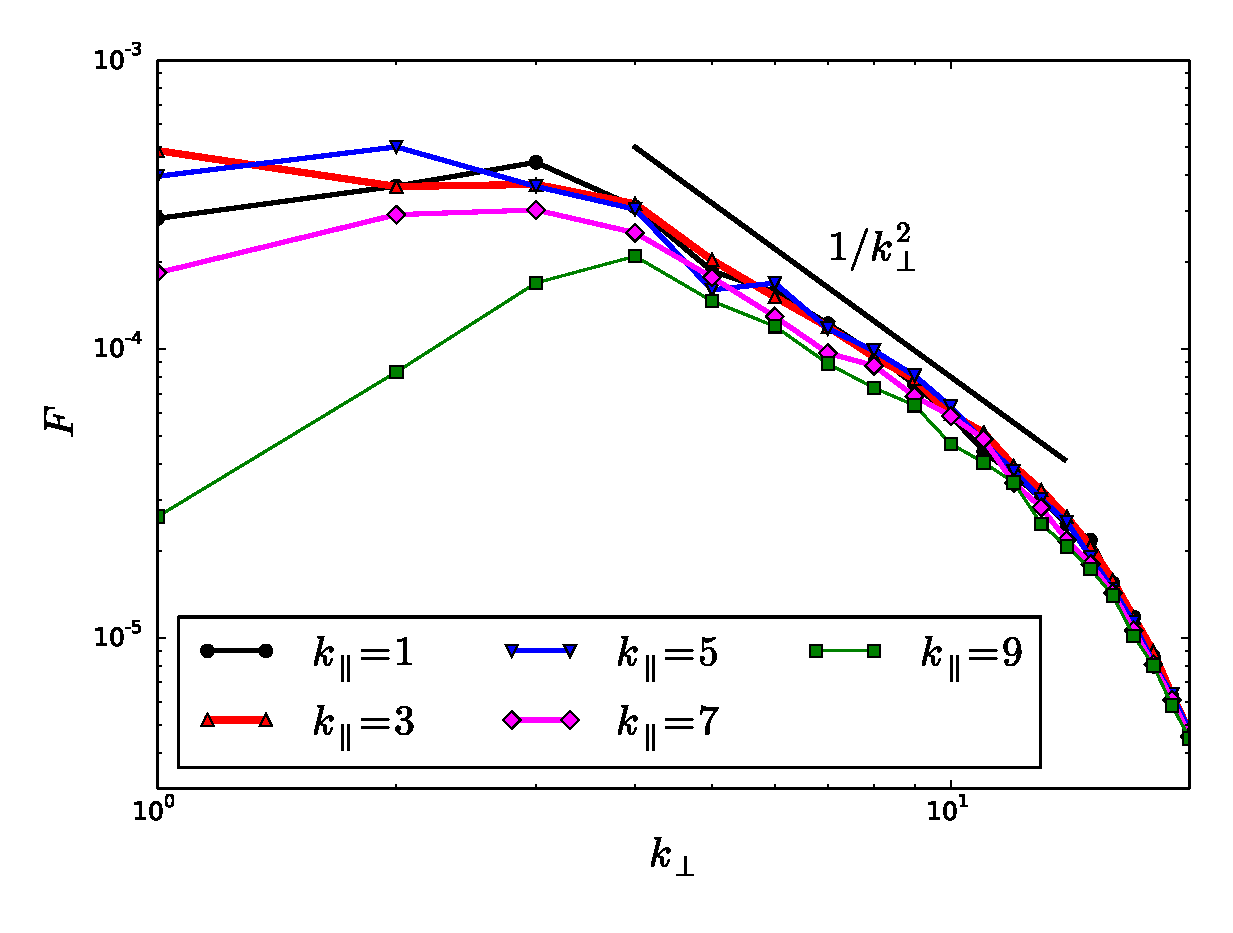
\includegraphics[width=14.8cm]{figs/phmixnl/M900_m100_vskp.eps}
        \caption{$\Fsk$ vs $k_\perp$ for $s=10$. $\Fsk$ increases for $k_\perp \leq \kpar/C_K$, and
        then is $\sim 1/k_\perp^2$.}
        \label{phmixnl:fig:m100f:vskp}
    \end{center}
    \end{figure}
    \begin{figure}
    \begin{center}
        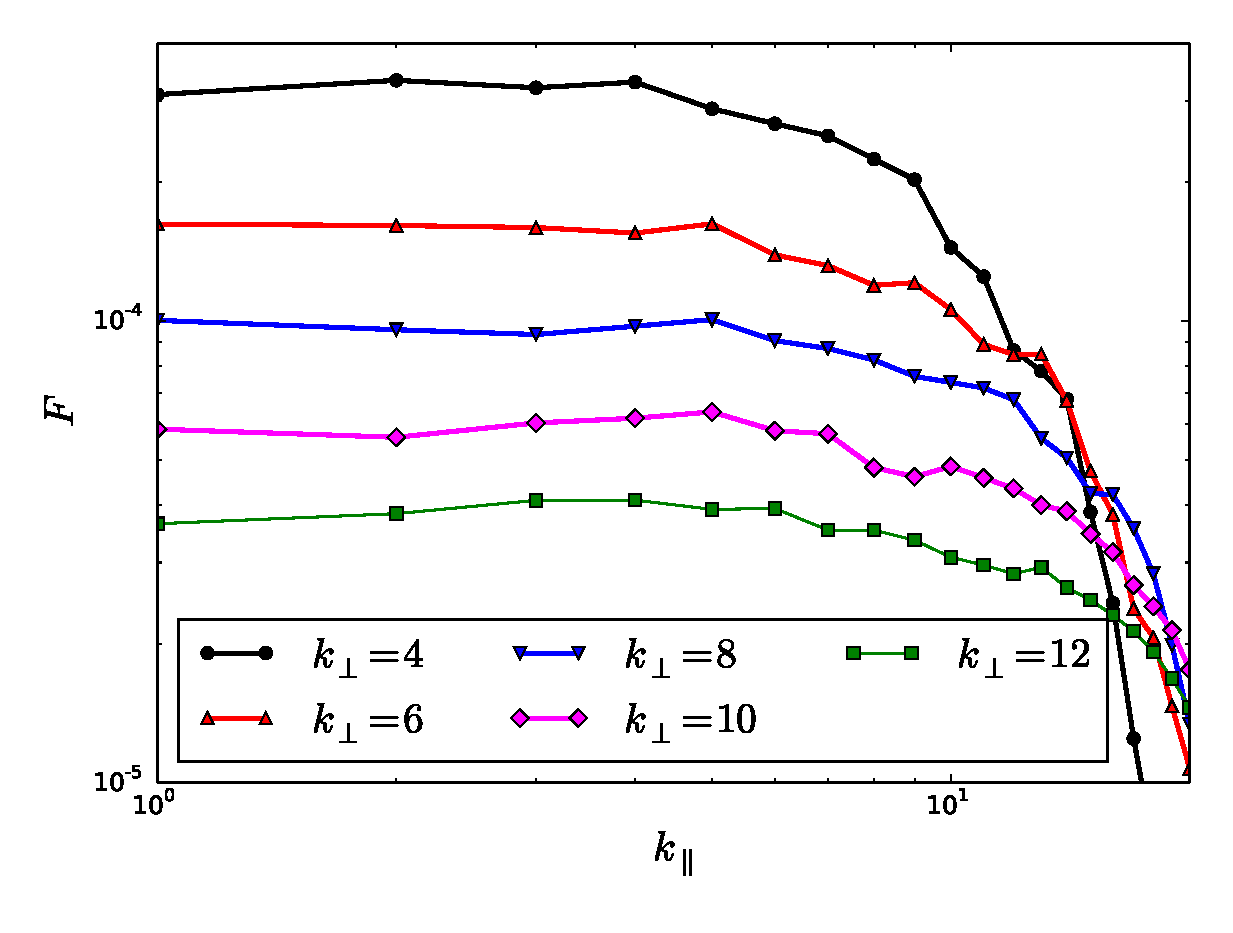
\includegraphics[width=14.8cm]{figs/phmixnl/M900_m100_vskz.eps}
        \caption{$\Fsk$ vs $\kpar$ for $s=10$. $\Fsk$ is a constant $\kpar \leq C_K k_\perp$, and
        then steeply rolls off.}
        \label{phmixnl:fig:m100f:vskz}
    \end{center}
    \end{figure}

   In the previous section we saw that the phase space is split into a suppressed and an
   unsuppressed region by the $\kpar^3 \sim k_\perp^2 \lt|s_c-s\rt|/\tau_C$ line. In this
   section we discuss how the spectra look like in the $(s, k_\perp, \kpar)$ phase space. 

    From \figref{phmixnl:fig:m100fpm:vskpkz}, we
    see that the phase-mixing component cascades to small spatial scales along the $\kpar
    \sim C_K k_\perp$ line\footnote{This may be thought of as the analog of a
    critical-balance style relationship between parallel and perpendicular wavenumbers in
    our model; $C_K$ is the equivalent Kolmogorov-constant.}, where $C_K$ is a constant (we observe $C_K\approx 2$). This
    relationship between the parallel and the perpendicular wavenumber can also be seen
    from the 1D spectra plotted in \figsand{phmixnl:fig:m100f:vskp}{phmixnl:fig:m100f:vskz}: the perpendicular
    spectra increase till $k_\perp \leq \kpar/C_K$, and then are approximately $\sim 1/k_\perp^2$,
    whereas the parallel spectra are constant till $\kpar \leq C_K k_\perp$ and then roll
    off steeply.

    In order to understand these spectra, we add the $``+"$ and $``-"$ equations in
    \eqref{phmixnl:eq:Fskpm}, to derive an equation for the spectrum $\Fsk$:
    \bea
        \pd{\Fsk}{t} + \pd{\Gsk}{s} + 2 \nu
        s^2 \Fsk + 2 \eta k_\perp^2 \Fsk =  
        \textit{Nonlinear terms}.
        \label{phmixnl:eq:Fsk}
    \eea
    For the suppressed region of the phase space, $\Gsk \approx 0$, i.e., the steady state
    spectrum is a zero flux solution. Setting $\Gsk=0$ in \eqref{phmixnl:eq:Fsk}
    reduces the problem to the fluid limit. It can be shown in this limit that the spectrum is given by $\Fsk
    \propto k_\perp/\lt(\kpar^2 + C_K^2 k_\perp^2\rt)^{3/2}$; this is consistent with the
    spectra observed in \figsand{phmixnl:fig:m100f:vskp}{phmixnl:fig:m100f:vskz}. 

    \begin{figure}
    \begin{center}
        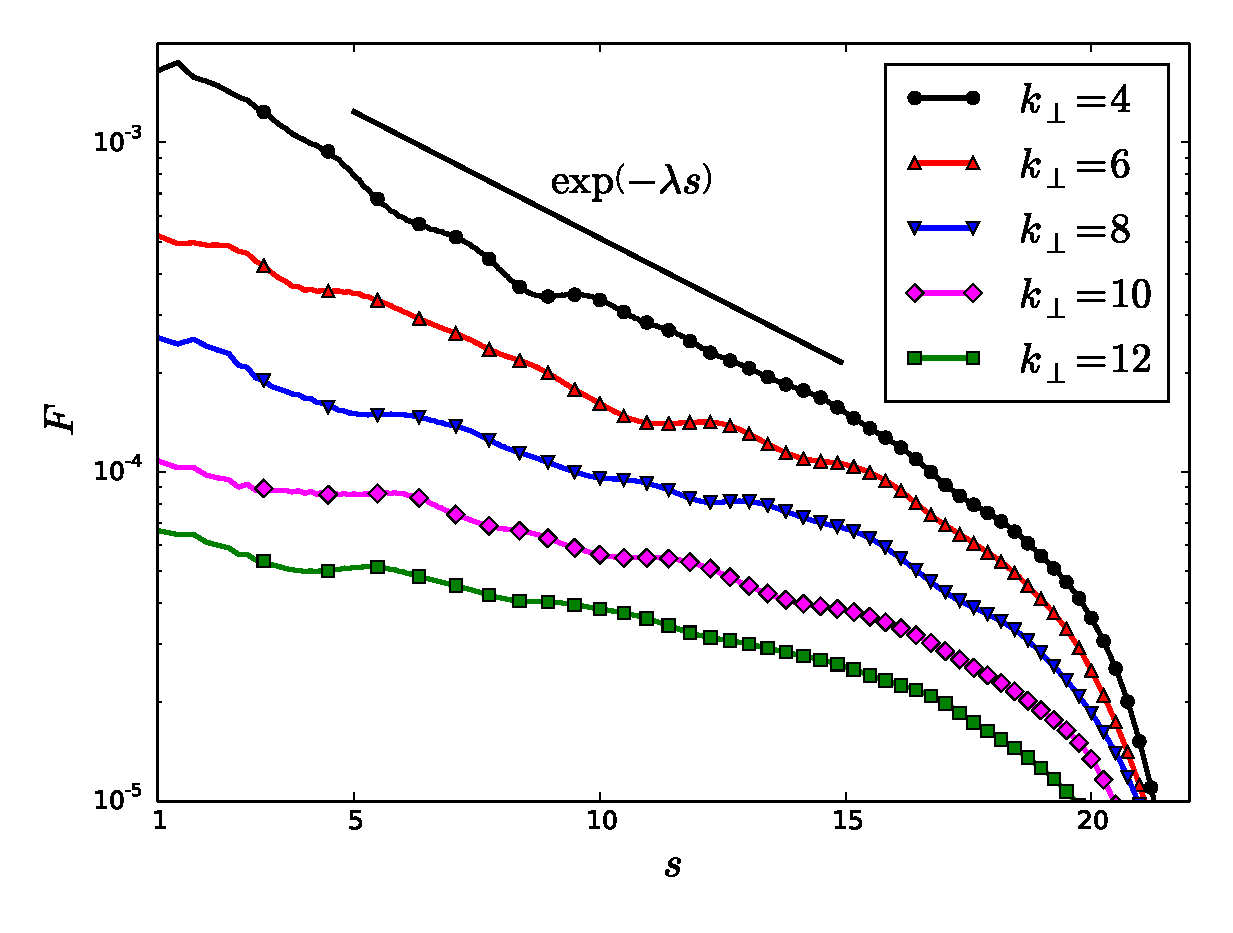
\includegraphics[width=14.8cm]{figs/phmixnl/M900_kz2_vss.eps}
        \caption{$\Fsk$ vs $s$ for $\kpar=2$. The spectrum decays in $s$ at a rate $\lambda \propto
        1/k_\perp$ (see \figref{phmixnl:fig:lambda:vskp}) in the region where phase-mixing is
        suppressed (see
        \figsdash{phmixnl:fig:m100supp:vskpkz}{phmixnl:fig:m100fpm:vsskp}).}
        \label{phmixnl:fig:m100f:kz2:vss}
    \end{center}
    \end{figure}
    \begin{figure}
    \begin{center}
        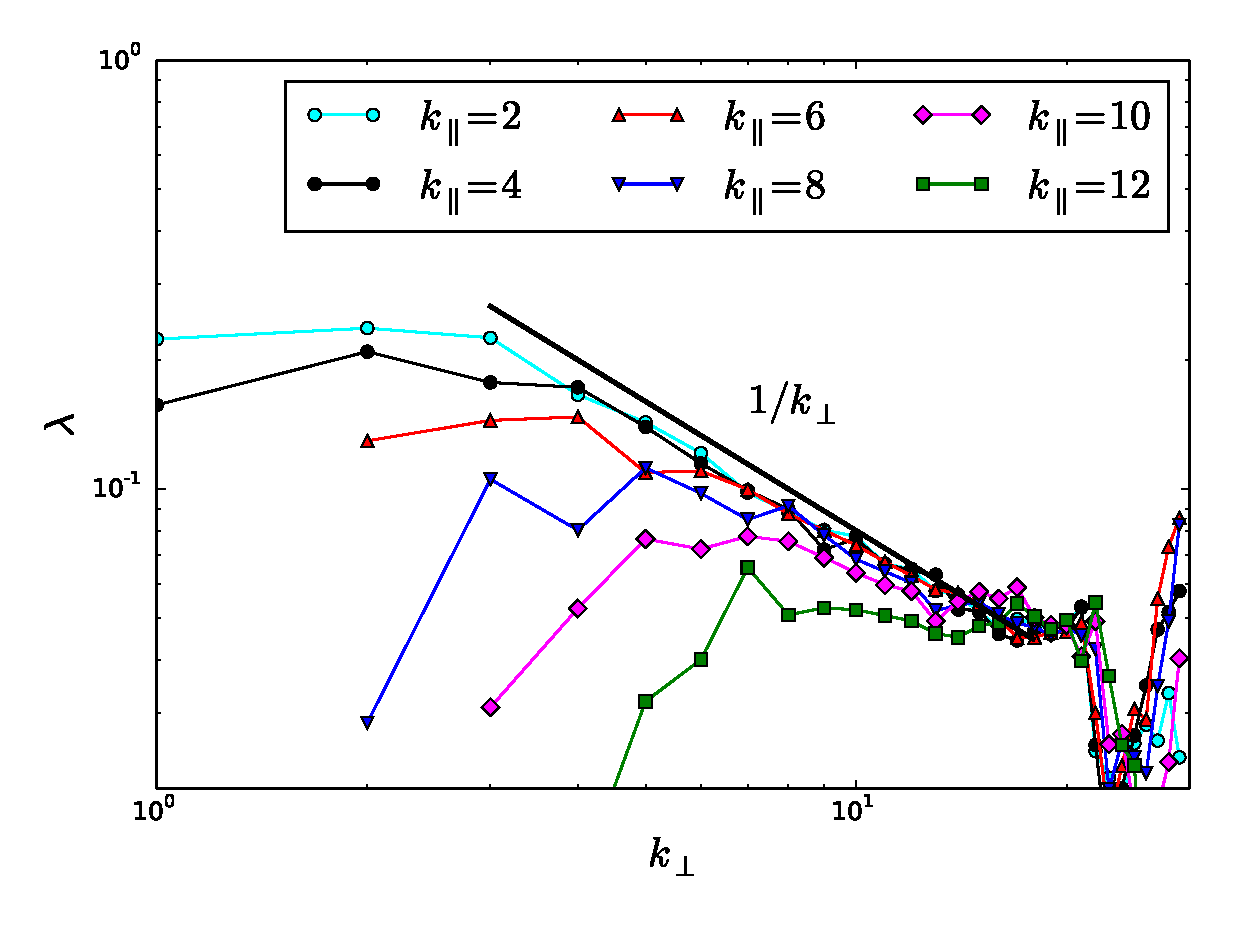
\includegraphics[width=14.8cm]{figs/phmixnl/M900_lambda_vskp.eps}
        \caption{The rate $\lambda$ at which spectrum $\Fsk$ decays in $s$ (see
        \figref{phmixnl:fig:m100f:kz2:vss}) vs $k_\perp$. We observe that $\lambda \propto
        1/k_\perp$ in the suppressed region; in the unsuppressed region $\lambda \approx
        0$.}
        \label{phmixnl:fig:lambda:vskp}
    \end{center}
    \end{figure}
    \begin{figure}
    \begin{center}
        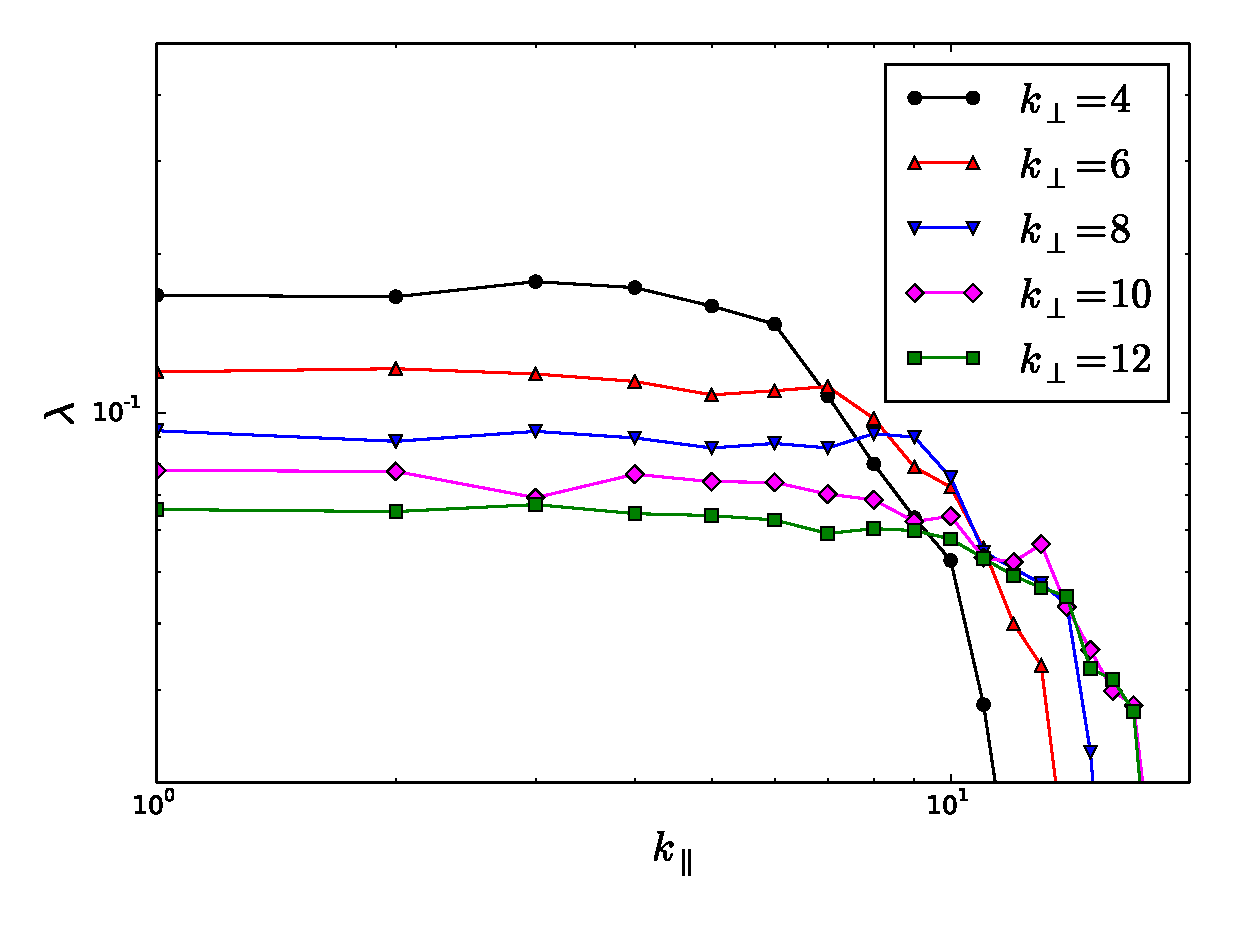
\includegraphics[width=14.8cm]{figs/phmixnl/M900_lambda_vskz.eps}
        \caption{The rate $\lambda$ at which spectrum $\Fsk$ decays in $s$ (see
        \figref{phmixnl:fig:m100f:kz2:vss}) vs $\kpar$. $\lambda$ is independent of $\kpar$ in the
        suppressed region; in the suppressed region $\lambda \to 0$.}
        \label{phmixnl:fig:lambda:vskz}
    \end{center}
    \end{figure}
    \begin{figure}
    \begin{center}
        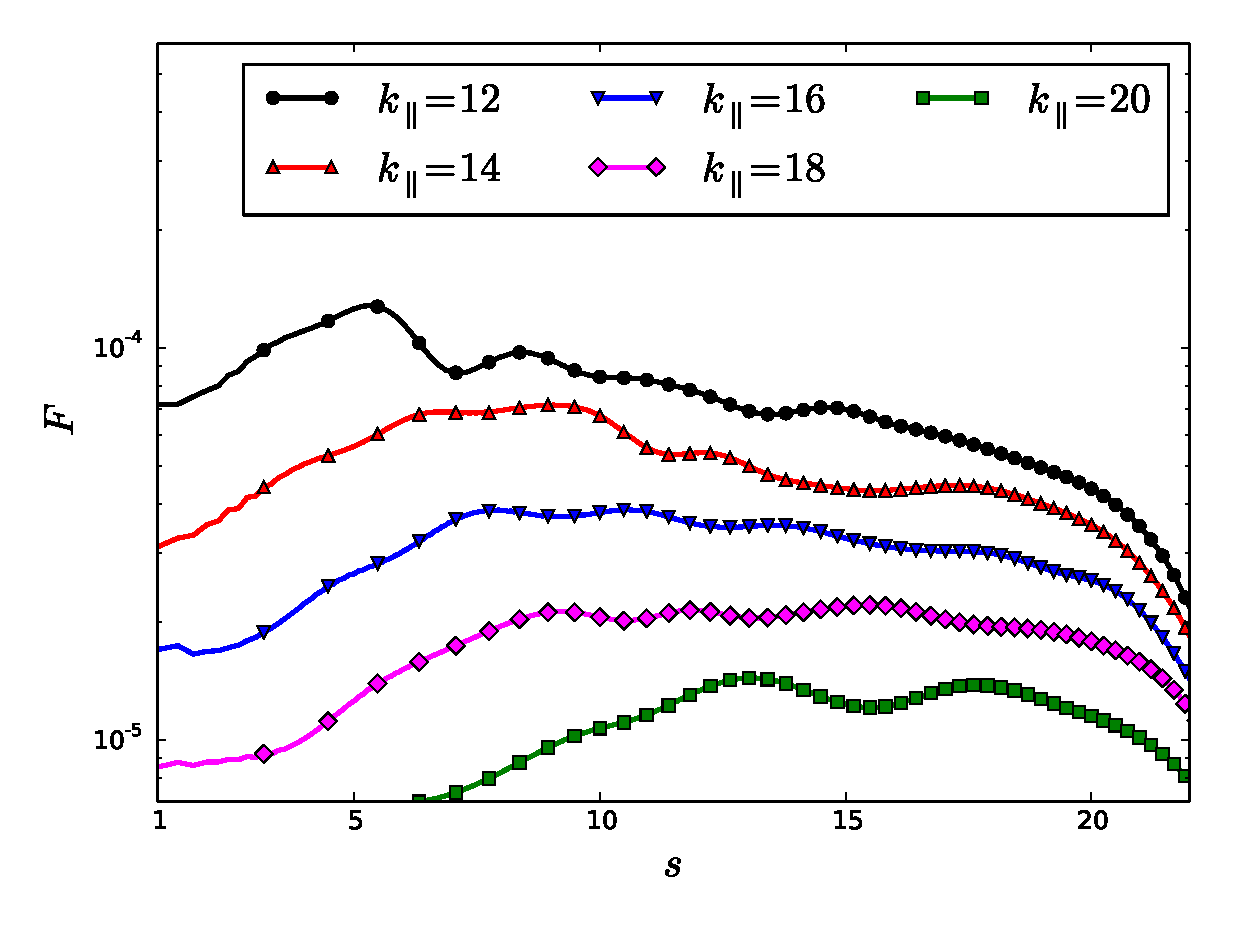
\includegraphics[width=14.8cm]{figs/phmixnl/M900_kp6_vss.eps}
        \caption{$\Fsk$ vs $s$ for $k_\perp=6$. In the unsuppressed region the
        spectrum vs $s$ is constant.}
        \label{phmixnl:fig:m100f:kp6:vss}
    \end{center}
    \end{figure}
    
    The spectra versus $s$ in the suppressed region are observed to decay exponentially 
     at a rate proportional to 
    $1/k_\perp$, and independent of $\kpar$ (see
    \figsref{phmixnl:fig:m100f:kz2:vss}{phmixnl:fig:lambda:vskp}{phmixnl:fig:lambda:vskz}).
    In the unsuppressed (phase-mixed) region, the $s$ spectrum is constant (see
    \figsref{phmixnl:fig:lambda:vskp}{phmixnl:fig:lambda:vskz}{phmixnl:fig:m100f:kp6:vss}), which is the
    same spectrum as that for the Landau-damped solution\footnote{Since the spectrum
    plotted in this chapter is $\Fsk=\sqrt{m}k_\perp|\tgmk|^2$, a constant-in-$s$ spectrum
    is same as the $|g_m|^2 \sim 1/\sqrt{m}$ spectrum from \chapref{chap:phmixlin}.} \cite{watanabe04, zocco11,
    hatch13, kanekar14a}.

%\subsection{$s=1$}
%    \begin{figure}
%    \begin{center}
%        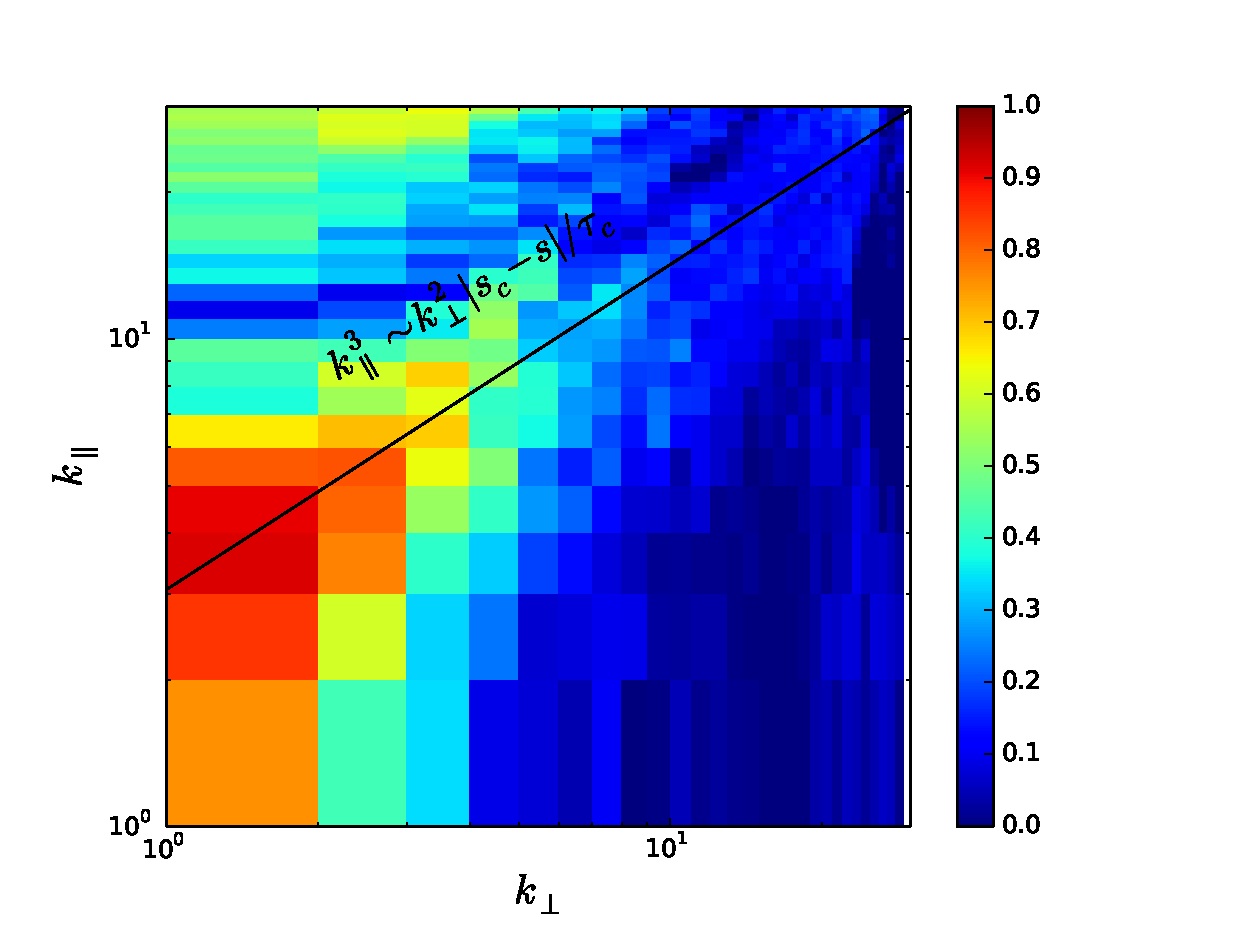
\includegraphics[width=14.8cm]{figs/phmixnl/M900_m1_exsupp_vskpkz.eps}
%        \caption{Exact normalized flux through $s=1$ vs $k_\perp-\kpar$}
%    \end{center}
%    \end{figure}
%    \begin{figure}
%    \begin{center}
%        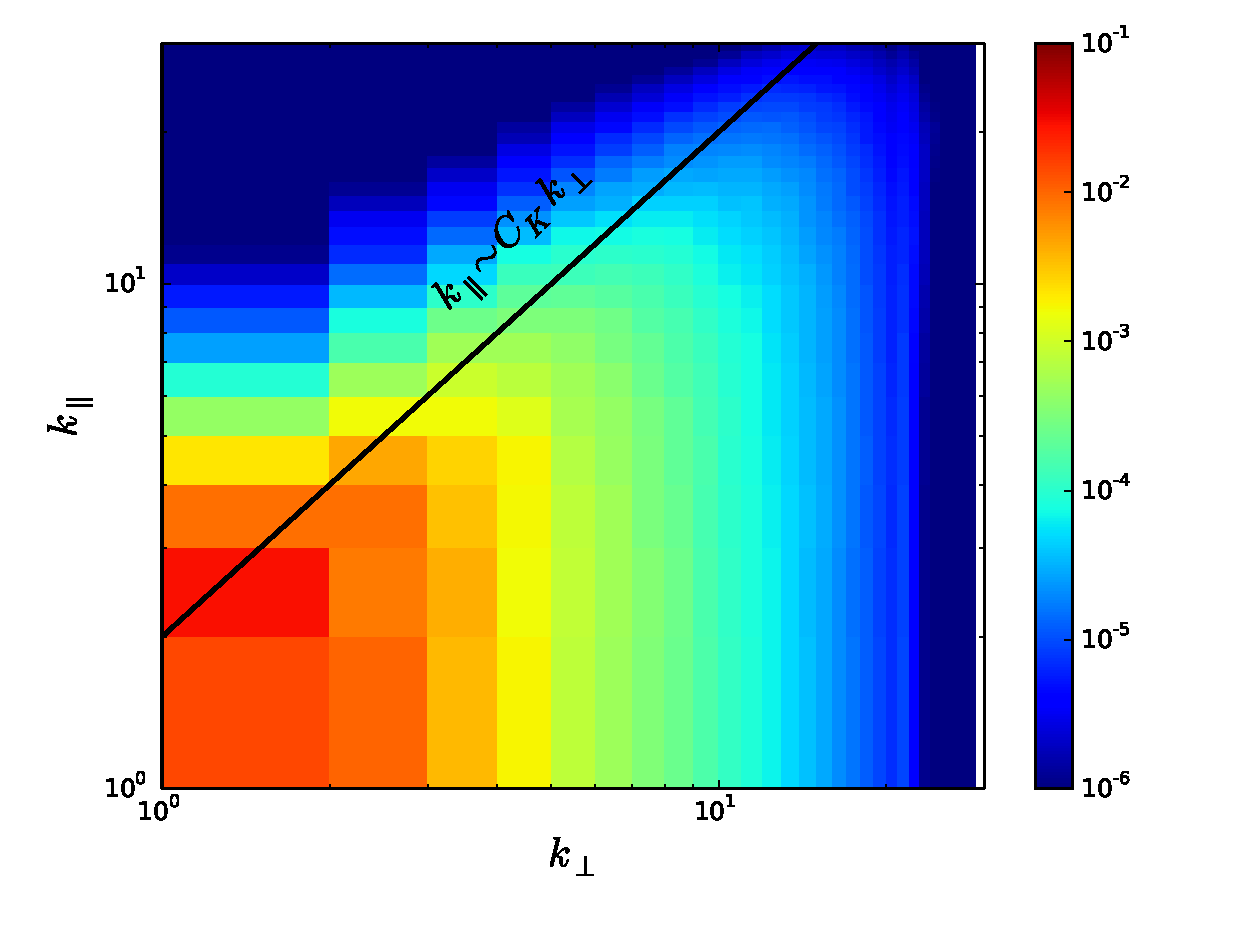
\includegraphics[width=14.8cm]{figs/phmixnl/M900_m1_f_vskpkz.eps}
%    \end{center}
%    \end{figure}
%    \begin{figure}
%    \begin{center}
%        \includegraphics[width=14.8cm]{figs/phmixnl/M900_m1_vskp.eps}
%    \end{center}
%    \end{figure}
%    \begin{figure}
%    \begin{center}
%        \includegraphics[width=14.8cm]{figs/phmixnl/M900_m1_vskz.eps}
%    \end{center}
%    \end{figure}
%    
%    \begin{figure}
%    \begin{center}
%        \includegraphics[width=14.8cm]{figs/phmixnl/M900_m1_vskpkz.eps}
%        \caption{Spectrum $\Fsk$ vs $k_\perp, \kpar$ at $s=1$ for parameters $\tauc
%        \simeq 1.5$, $s_c \simeq 17.5$, $k_{\perp, \eta} = 17.4$. The energy cascade proceeds
%        along the $\kpar \sim C_K k_\perp$ line; most of the energy is contained within
%        the cone below this line ($\kpar \leq C_K k_\perp$).}
%        \label{phmixnl:fig:kpkzspec}
%    \end{center}
%    \end{figure}
%    \begin{figure}
%    \begin{center}
%        \includegraphics[width=14.8cm]{figs/phmixnl/M900_m1_vskp.eps}
%        \caption{Perpendicular spectrum at $s=1$ for parameters $\tauc
%        \simeq 1.5$, $s_c \simeq 17.5$, $k_{\perp, \eta} = 17.4$. For $\kpar \leq C_K
%        k_\perp$ the spectrum is $\sim 1/k_\perp^2$.} 
%        \label{phmixnl:fig:1dkpspec}
%    \end{center}
%    \end{figure}
%    \begin{figure}
%    \begin{center}
%        \includegraphics[width=14.8cm]{figs/phmixnl/M900_m1_vskz.eps}
%        \caption{Parallel spectrum at $s=1$ for parameters $\tauc
%        \simeq 1.5$, $s_c \simeq 17.5$, $k_{\perp, \eta} = 17.4$. For $\kpar \leq C_K
%        k_\perp$ the parallel spectrum is constant.}
%        \label{phmixnl:fig:1dkzspec}
%    \end{center}
%    \end{figure}
%
%    The cascade in real space is observed to proceed along the
%    $\kpar\sim~C_K~k_\perp$ line (see
%    \figref{phmixnl:fig:kpkzspec}), where $C_K$ is a constant that relates the parallel and
%    perpendicular wavenumbers \footnote{Scaling argument}; in our simulations we observe $C_K \approx 2$.  
%    Most of the energy in the system is contained within the
%    $\kpar \leq C_K k_\perp$ region. The relationship between the parallel and
%    perpendicular wavenumbers can also be seen from 1D spectra shown in
%    \figsand{phmixnl:fig:1dkpspec}{phmixnl:fig:1dkzspec}. The perpendicular spectrum at a fixed parallel
%    wavenumber $\kpar$ increases till $k_\perp \leq \kpar/C_K$, beyond which it goes as
%    $1/k_\perp^2$. The parallel spectrum at a fixed wavenumber $k_\perp$ remains constant
%    till $\kpar \leq C_K k_\perp$, and falls off rapidly for larger parallel wavenumbers.
%    These 1D spectra reaffirm the assertion that $\kpar \leq C_K k_\perp$ is the
%    energetically relevant region of the phase space for our model.
%
%    \begin{figure}
%    \begin{center}
%        \includegraphics[width=14.8cm]{figs/phmixnl/M900_kz2_vss.eps}
%        \caption{Spectrum vs $s$ for parameters $\tauc
%        \simeq 1.5$, $s_c \simeq 21.3$, $k_{\perp, \eta} = 17.4$, $\kpar=2$. The spectrum
%        decays exponentially in $s$ at a
%        rate $\lambda\lt(k_\perp,\kpar\rt)$ for $\kpar\leq C_K k_\perp$.} 
%        \label{phmixnl:fig:1dsspec}
%    \end{center}
%    \end{figure}
%
%    \begin{figure}
%    \begin{center}
%        \includegraphics[width=14.8cm]{figs/phmixnl/M900_lambda_vskp.eps}
%        \includegraphics[width=14.8cm]{figs/phmixnl/M900_lambda_vskz.eps}
%        \caption{The decay rate $\lambda$ (see \figref{phmixnl:fig:1dsspec}) is independent of
%        $\kpar$, and is inversely proportional to $k_\perp$.}
%        \label{phmixnl:fig:1dsspec:lambda}
%    \end{center}
%    \end{figure}
%
%    The $s$ spectrum for $\kpar^3~\leq~\tauc~k_\perp^2~s_c$ decays exponentially at a rate
%    inversely proportional to $k_\perp$ and independent of $\kpar$ (see 
%    \figsand{phmixnl:fig:1dsspec}{phmixnl:fig:1dsspec:lambda}). For $\kpar~\geq~C_K k_\perp$, the $s$
%    spectrum is constant (see \figref{phmixnl:fig:1dsspec:2}).
%
%    \begin{figure}
%    \begin{center}
%        \includegraphics[width=14.8cm]{figs/phmixnl/M900_kp6_vss.eps}
%        \caption{Spectrum vs $s$ for parameters $\pu
%        \simeq 1.5$, $s_c \simeq 21.3$, $k_{\perp, \eta} = 17.4$, $k_\perp=6$. After an
%        initial ``transient", the spectrum is constant in $s$ for $\kpar\geq C_K k_\perp$.} 
%        \label{phmixnl:fig:1dsspec:2}
%    \end{center}
%    \end{figure}
%
    
%    This comes about as a
%    result of the competition between linear phase-mixing and the nonlinear turbulent
%    cascade.  Phase-mixing tries to drive the system towards a constant-in-$s$ spectrum
%    \cite{watanabe04, zocco11, hatch13, kanekar14a} on
%    an inverse timescale proportional to $\kpar\vth\sim~C_K~k_\perp\vth$, while the
%    nonlinear cascade transfers energy to large $\mb{k}$ at a rate $\pu$, attempting to
%    prevent any flux to high $s$; which results in the observed spectrum $\Fsk\sim\exp\lt(-\pu
%    s/\lt(C_K k_\perp \vth\rt)\rt)$.  For $\kpar~\geq~C_K k_\perp$,
%    the system is seen to approach a constant-in-$s$ spectrum (see
%    \figref{phmixnl:fig:1dsspec:3}).   

%\subsection{Flux in Hermite space}
%
%    To understand the numerically observed spectra from the previous section, we derive an equation for the spectrum
%    $\Fsk~=~\sqrt{m}k_\perp|\tgmk|^2$ by adding $``+"$
%    and $``-"$ equations in \eqref{phmixnl:eq:Fskpm} to obtain,
%    \bea
%        \pd{\Fsk}{t} + \pd{\Gsk}{s} + 2 \nu s^2 \Fsk + 2 \eta k_\perp^2 \Fsk =  \nonumber \\
%        \textit{Nonlinear terms}.
%        \label{phmixnl:eq:Fsk}
%    \eea
%    The second term on the left hand side of \eqref{phmixnl:eq:Fsk} describes the flux of energy to higher
%    Hermite moments; ignoring this term is equivalent to taking the fluid limit.
%    Interestingly, the spatial spectra observed in the previous section are same as
%    that for the fluid passive scalar: $\Fsk~\propto~k_\perp/\lt(\kpar^2 + C_K^2
%    k_\perp^2\rt)^{3/2}$. This suggests a constant flux steady state solution.
%    
%    \begin{figure}
%    \begin{center}
%        \includegraphics[width=14.8cm]{figs/phmixnl/M36_exsupp_m1_vskpkz.eps}
%        \includegraphics[width=14.8cm]{figs/phmixnl/M100_exsupp_m1_vskpkz.eps}
%        \caption{Normalized flux of free energy in Hermite space
%        $\Gsk/\lt(\sqrt{2}|\kpar|\vth \Fsk\rt)$ vs $k_\perp, \kpar$ at $s=1$ for
%        parameters $\pu \simeq 1.5$, $k_{\perp, \eta} = 17.4$. The top figure corresponds
%        to $s_c \sim 4.7$, and the bottom figure $s_c \sim 7.6$. Phase-mixing is nearly
%        completely suppressed in the region given by
%        $\kpar^3 \leq \pu k_\perp^2 |s_c-s|$.}
%    \label{phmixnl:fig:supp1} 
%    \end{center}
%    \end{figure}
%    \begin{figure}
%    \begin{center}
%        \includegraphics[width=14.8cm]{figs/phmixnl/M400_exsupp_m1_vskpkz.eps}
%        \includegraphics[width=14.8cm]{figs/phmixnl/M900_exsupp_m1_vskpkz.eps}
%        \caption{Normalized flux of free energy in Hermite space
%        $\Gsk/\lt(\sqrt{2}|\kpar|\vth \Fsk\rt)$ vs $k_\perp, \kpar$ at $s=1$ for
%        parameters $\pu \simeq 1.5$, $k_{\perp, \eta} = 17.4$. The top figure corresponds
%        to $s_c \sim 14.2$, and the bottom figure $s_c \sim 21.3$. Phase-mixing is nearly
%        completely suppressed in the region given by
%        $\kpar^3 \leq k_\perp^2 |s_c-s|$.}
%        \label{phmixnl:fig:supp2}
%    \end{center}
%    \end{figure}
%    \begin{figure}
%    \begin{center}
%        \includegraphics[width=14.8cm]{figs/phmixnl/M900_fpm_m1_vskpkz.eps}
%        \caption{Spectrum $\Fsk^\pm$ at $s=1$ vs $k_\perp, \kpar$ for parameters $\pu
%        \simeq 1.5$, $s_c \simeq 17.5$, $k_{\perp, \eta} = 17.4$. The phase-unmixing
%        spectrum $\Fsk^-$ is plotted on the left, whereas the phase-mixing spectrum
%        $\Fsk^+$ is plotted on the right.
%        The two components nearly cancel eachother in the trianglular region given by
%        $\kpar^3 \leq \pu k_\perp^2 s_c$, resulting in nearly zero net flux into Hermite space.} 
%        \label{phmixnl:fig:fpm:kpkzspec}
%    \end{center}
%    \end{figure}
%
%    \begin{figure}
%    \begin{center}
%        \includegraphics[width=14.8cm]{figs/phmixnl/N64_coll_m4kp12_vskz.eps}
%        \includegraphics[width=14.8cm]{figs/phmixnl/N64_coll_m49kp12_vskz.eps}
%        \caption{Spectrum $\Fsk^\pm$ vs $\kpar$ at $k_\perp=12$, for two different
%        collisionalities. The top plot is for $s=2$, whereas the bottom plot is for $s=7$.
%        For $s=2$, the two spectra nearly coincide proving convergence. However, for
%        $s=7$, there is substantially less energy in the phase-unmixing mode for the
%        collisional case as compared to the collisionless case. Collisional effects also
%        modify the $\kpar$ spectrum, since the solution is no longer the zero-flux
%        solution.}
%        \label{phmixnl:fig:coll:vskz}
%    \end{center}
%    \end{figure}
%
%    Net flux through the first Hermite moment is observed to be nearly zero for
%    wavenumbers in the range $\kpar^3 \leq \pu k_\perp^2 s_c$ (see
%    \figsand{phmixnl:fig:supp1}{phmixnl:fig:supp2}). In this region, the free energy is nearly
%    equally partitioned between the phase-mixing and the phase-unmixing components, 
%     (see \figref{phmixnl:fig:fpm:kpkzspec}),  demonstrating that the stochastic plasma echo is responsible
%     for the zero flux solution. 
%
%    \begin{figure}
%    \begin{center}
%        \includegraphics[width=14.8cm]{figs/phmixnl/M900_exsupp_kp8_vsskz.eps}
%        \includegraphics[width=14.8cm]{figs/phmixnl/M900_exsupp_kz8_vsskp.eps}
%        \caption{Normalized flux of free energy in Hermite space
%        $\Gsk/\lt(\sqrt{2}|\kpar|\vth \Fsk\rt)$ for parameters $\pu \simeq 1.5$,
%        $k_{\perp, \eta} = 17.4$, $s_c \sim 21.3$, plotted vs $s-\kpar$ at $k_\perp=8$ in
%        the top plot, and vs $s-k_\perp$ at $\kpar=8$ in the bottom plot. The suppressed
%        region is given by $\kpar^3 \leq \pu k_\perp^2 |s_c - s|$.}
%        \label{phmixnl:fig:supp3}
%    \end{center}
%    \end{figure}
%     
%     The extent of the suppressed region is
%     determined by the collisionality of the system. Collisional dissipation
%    extracts energy from a phase-mixing mode before it can couple to an phase-unmixing
%    mode. This sets an upper bound in $\kpar$, given by $k_{\parallel, c} \sim
%    \lt(\pu k_\perp^2 \lt|s_c-s\rt|\rt)^{1/3}$, beyond which there is no 
%    energy in the phase-unmixing modes, resulting in finite non-zero flux into Hermite
%    space (see \figref{phmixnl:fig:supp3}). 
%    
%    This deviation from the zero-flux solution can also be gleaned from the parallel
%    spectra plotted in \figref{phmixnl:fig:coll:vskz}---parallel spectrum for the more
%    collisional system is not the same as that for the fluid passive scalar, this is also
%    the part of phase space where phase-mixing is not suppressed.
%     %This can also be diagnosed by looking at
%     %the behavior of the system at different values of $s$ in the same simulation; since
%     %the dynamics in the Hermite space is universal (see \eqref{phmixnl:eq:gmeq}), looking at the
%     %spectra and suppression at a higher value of $s$ is roughly equivalent to studying a
%     %a more collisional system.
%
%
%    %\begin{figure*}
%    %\begin{center}
%    %    \includegraphics[width=18cm]{figs/phmixnl/M900_mat_vss.eps}
%    %    \caption{Spectrum vs $s$ for parameters $\pu
%    %    \simeq 1.5$, $s_c \simeq 17.5$, $k_{\perp, \eta} = 17.4$, for multiple values of
%    %    $k_\perp, \kpar$. The numbers in the top right corner of each little plot denote
%    %    the $(k_\perp, \kpar)$ values. The dotted line plots $\exp(-\pu s/(2 k_\perp
%    %    \vth)$.} 
%    %    \label{phmixnl:fig:sspec:mat}
%    %\end{center}
%    %\end{figure*}
%
%    
%
%%    The zero-flux solution discussed above is true for values of $s$ where collisions can
%%    be safely ignored. For larger $s$, collisional dissipation
%%    extracts energy from a phase-mixing mode before it can couple to an phase-unmixing
%%    mode. This effectively sets an upper bound in $\kpar$ beyond which there is no 
%%    phase-unmixing mode, resulting in finite non-zero
%%    flux into Hermite space. This deviation from the zero-flux solution can be seen from the parallel spectra plotted in \figref{phmixnl:fig:coll:vskz}.
%%
%    \begin{figure}
%    \begin{center}
%        \includegraphics[width=14.8cm]{figs/phmixnl/M900_visc_kp4kz4_vss.eps}
%        \includegraphics[width=14.8cm]{figs/phmixnl/M900_visc_kp8kz4_vss.eps}
%        \caption{Spectrum $\Fsk$ vs $s$ at $k_\perp=12$, for two different
%        viscosities. The top plot is for $k_\perp=4, \kpar=4$, whereas the bottom plot
%        is for $k_\perp=8, \kpar=4$.
%        For $k_\perp=4, \kpar=4$, the two spectra nearly coincide proving convergence. However, for
%        $k_\perp=8, \kpar=4$, the spectrum for the viscous case is steeper.}
%        \label{phmixnl:fig:visc:vss}
%    \end{center}
%    \end{figure}
%
%    We discussed the effect of collisional dissipation on the steady-state solution of our
%    model. Finite viscous effects modify the solution as well---
%    viscosity sets a cutoff in $k_\perp$, which in turn sets a cutoff in $\kpar$; as a
%    result the $s$ spectrum for modes close to the viscous cutoff have a steeper $s$
%    spectrum as shown in \figref{phmixnl:fig:visc:vss}.
    
\section{Conclusions and discussion}

    We demonstrated with a simplified model for kinetic passive scalar turbulence that
    Landau damping, or more generally phase mixing can be suppressed significantly in
    turbulent systems for a part of the phase space. Energy is scattered in the phase
    space such that the net flux to higher Hermite moments of the distribution
    function is reduced due to the stochastic plasma echo.
    We showed using direct numerical simulations that phase mixing is 
    suppressed significantly in the region $\kpar^3 \leq \pu k_\perp^{2/3} s_c$.
    Therefore, in the collisionless limit ($s_c \to \infty$), phase mixing would be suppressed
    in the whole inertial range.
    Perpendicular and parallel spectra were shown to be the same as fluid spectra in the
    suppressed region.
    The suppression of Landau damping by the stochastic plasma echo helps explain why
    power law energy spectra survive at scales where fluctuations are expected to be
    strongly damped, by linear theory.

    Here, we conclude our
    treatment of the kinetic passive scalar (chapters \ref{chap:phmixlin}, \ref{chap:pp0}
    and \ref{chap:phmixnl}), and give a summarized list of our results so
    far:
    \begin{itemize}
        \item We analytically derived the fluctuation-dissipation relations in the linear
        limit for the kinetic passive scalar.

        \item We constructed an analytical framework to diagnose the efficiency of phase
        mixing by considering the flow of energy in the Hermite space. Within this
        framework, we proved that
        in the linear limit, the steady state solution to the system is a constant-flux
        solution, and that the energy solely flows from small to large Hermite moments for
        large values of $\sqrt{m}$.

        \item When the passive scalar is being mixed by a 2D velocity field,
        the spectrum in the Hermite space is exponentially attenuated in the strong turbulence regime, and the
        behavior of the kinetic system is essentially fluid-like. This is a result of the
        energy in the passive scalar being swept up to small spatial scales by the
        advecting velocity field, before it can phase mix.

        \item On the other hand, if the scalar is being mixed by a 3D velocity, there is a stochastic analog of the plasma
        echo which suppresses the 
        efficiency of phase mixing in a part of the phase space, the
        extent of which is determined by the collisionality of the system, and the
        amplitude of the advecting velocity. 
    \end{itemize}

    In the next chapter, we use these ideas, and the diagnostic tools developed here to study the compressive
    fluctuations cascade in the kinetic reduced MHD limit.
    

%\renewcommand{\thechapter}{7}
\chapter{Compressive fluctuations in the solar wind}
\label{chap:slowmodes}
\section{Introduction}
\label{slowmodes:sec:intro}

    In situ measurements of turbulence in the solar wind \cite{coleman68,
    matthaeus82,bale05, podesta07,tessein09,podesta10}  make it a remarkable laboratory
    to study kinetic plasma turbulence. It is generally agreed upon
    that the turbulence in the solar wind comprises mostly of Alfv\'{e}nic fluctuations
    \cite{belcher71} (about
    90\% of the energy), with an admixture of compressive modes. The Alfv\'{e}n-wave cascade has been studied in
    great detail using fluid \cite{kinney98, cho00, maron01, cho02, dmitruk03, muller03,
    haugen04, oughton04, muller05, mason08, perez08, beresnyak11, beresnyak11prl, mason11,
    mason12, perez12} and kinetic \cite{howes08pop, howes08prl, nielson13} models.
    Numerical studies of the compressive cascade have mostly been done in the
    fluid limit \cite{lithwick01, cho02prl, cho03, beresnyak05, cho05, kowal07}. However,
    since the solar wind is a nearly collisionless plasma, a kinetic treatment is
    required. The compressive perturbations in the solar wind are mostly slow and entropy
    modes with negligible amounts of energy in the fast mode \cite{klein12}, hence a low
    frequency description like kinetic reduced MHD (which orders the fast mode out) can be used.

    \begin{figure}
    \begin{center}
        \includegraphics[width=12cm]{figs/slowmodes/slow_parallel_cascade.png}
        \caption{The compressive fluctuations are passively cascaded by the Alfv\'{e}nic
        turbulence, and may remain correlated along the perturbed fieldlines (figure taken
        from Schekochihin et al. \cite{tome}).}
        \label{slowmodes:fig:slow_par}
    \end{center}
    \end{figure}

    In a weakly collisional system like the solar wind, slow modes are subject
    to strong kinetic damping. This is at odds with the observed power law spectra for density and
    field strength fluctuations. Power law spectra suggest that compressive fluctuations undergo a Kolmogorov-style
    turbulent cascade. A possible explanation for this apparent discrepancy is 
    that even though slow modes develop fine scales in the plane perpendicular to the local magnetic
    field as they are passively mixed by the background Alfv\'{e}nic turbulence, they
    remaining correlated in the parallel direction \cite{tome}. 
    This leads to highly
    anisotropic structures with the parallel wavelength set by the initial conditions,
    which results in weak damping since the damping rate is proportional to the parallel
    wavenumber (see \figref{slowmodes:fig:slow_par}). However, this argument ignores 
    dissipation. Lithwick and Goldreich \cite{lithwick01}
    argued against this suggestion, by 
    noticing that when the cascade reaches the ion Larmor radius in the perpendicular
    plane, these highly anisotropic fluctuations would decorrelate due to finite Larmor
    radius effects (which in our model show up as a diffusive term at small perpendicular
    scales), and acquire the same parallel correlation
    lengths as the Alfv\'{e}n waves. Recent observations of the solar wind seem to support the idea that there is no
    parallel cascade \cite{chen11}. However, these results are somewhat inconclusive. In Chen
    \etal\, \cite{chen11}, they construct a representative eddy for the field strength
    fluctuations, and find it to be much more anisotropic than the Alfv\'{e}nic eddy (see
    their figures 4 and 6), which on its surface seems to have settled the issue. But in
    the same paper, they also observe a power law spectrum in the direction of the local
    magnetic field,
    with a spectral exponent between $-1.42$ and $-1.58$ (see their figure 5)---a shallower spectrum than
    that for Alfv\'{e}nic fluctuations (though severely limited by resolution). In fact
    they use this shallow spectrum to construct the eddy in
    the first place. A possible conciliation between these two mutually contradictory
    results is that the compressive fluctuations are
    anisotropic at the outer scale itself, and then cascade to smaller perpendicular and
    parallel scales \cite{chen14}---i.e., an anisotropic structure observed at small
    scales does not imply a lack of parallel cascade, and might be a result of the
    initial conditions.
    This however, still leaves two questions unanswered ---
    \begin{inparaenum}[(a)]
    \item is there a parallel cascade for the compressive fluctuations?
    \item If there is a parallel cascade, why are the compressive fluctuations undamped?
    \end{inparaenum}
    
    We show, using direct numerical simulations of kinetic reduced MHD, that the
    compressive fluctuations undergo a parallel cascade\footnote{The observed parallel
    cascade may be a result of our forcing---this requires further investigation. However,
    the results from \chapref{chap:pp0} explain the observed power law density fluctuation
    spectra for the case where there is no parallel cascade.}, but they remain
    undamped due to suppression of phase mixing by the turbulent plasma echo discussed in
    \chapref{chap:phmixnl}.

\section{Numerics} 

We solve \eqsand{intro:krmhd:els}{intro:krmhd:gpm} using \Gand. Alfv\'{e}n waves were
driven by injecting random velocity fluctuations using a Gaussian white noise source; 
compressive fluctuations were sourced independently by driving $\dBpar$, i.e. the zeroth
velocity moment of $g_B$ (see \eqref{eqs:eq:gnBdef}). The ion charge ($Z$), ion to electron
temperature ratio ($\tau$) and the ion plasma beta ($\beta_i$) were all set to 
one---these choices are representative of the usual solar wind parameters.
The resolution in the real space was
chosen to be $128^3$, $144$ Hermite moments of the perturbed distribution function were
evolved, hypercollisions ($\nu m^8$) and hyperviscosity
($\eta k_\perp^{16}$) were used to regularize fine scale structure.

\section{Alfv\'{e}nic turbulent cascade}

\begin{figure}
\begin{center}
    \includegraphics[width=7.4cm]{figs/slowmodes/sw1_alf_kpspec.eps}
    \includegraphics[width=7.4cm]{figs/slowmodes/sw1_alf_kparspec.eps}
    \caption{Perpendicular and parallel spectra of the Alfv\'{e}nic fluctuations. The
    critical balance predictions: $k_\perp^{-5/3}$ for the perpendicular spectra and
    $\kpar^{-2}$ for the parallel spectra are observed in simulations.}
\label{slowmodes:fig:alfspec} 
\end{center}
\end{figure}

    The Goldreich-Sridhar critical balance theory \cite{goldreich95, goldreich97, tome} predicts the Alfv\'{e}nic turbulence to
    have $k_\perp^{-5/3}$ perpendicular, and $\kpar^{-2}$ parallel spectra. The
    precise spectral exponent is a highly debated issue in the community---Boldyrev
    et al.\cite{boldyrev05, boldyrev06, boldyrev09, boldyrev11} argue that 
    scale-dependent dynamic alignment needs to be included in the critical-balance theory
    for MHD turbulence, which ends up predicting a $k_\perp^{-3/2}$ perpendicular
    spectrum, whereas Beresnyak et al. \cite{beresnyak11, beresnyak11prl} observe the
    Goldreich-Sridhar $k_\perp^{-5/3}$ spectrum in their simulations. The resolution requirements to settle this controversy are
    beyond the capability of present day GPUs, and hence this issue is not addressed in
    our work. In our simulations, we observe the perpendicular spectrum to be $k_\perp^{-5/3}$ (see
    \figref{slowmodes:fig:alfspec}), which we consider to be consistent with the
    theories on either side of this debate.
    The parallel spectrum is seen to be $\kpar^{-2}$ (see
    \figref{slowmodes:fig:alfspec}), which is a
    prediction of both the theories. Our numerical spectra
    are broadly consistent with observations in the solar wind \cite{matthaeus82, bale05,
    podesta07, tessein09, podesta10, chen10, chen11}.

\begin{figure}
\begin{center}
    \includegraphics[width=7.4cm]{figs/slowmodes/sw1_u2_kparkp.eps}
    \includegraphics[width=7.4cm]{figs/slowmodes/sw1_b2_kparkp.eps}
    \caption{Kinetic (left) and magnetic (right) energy  vs $k_\perp, \kpar$.}
\label{slowmodes:fig:alfanis} 
\end{center}
\end{figure}

    In addition to the power law spectra having different spectral exponents in the
    perpendicular and the parallel directions, the wavenumber anisotropy predicted by
    critical-balance can also be seen in the 2D spectra plotted in
    \figref{slowmodes:fig:alfanis}. The energy containing region is seen
    to bounded by the $\kpar \sim k_\perp^{2/3}$ line as predicted by critical
    balance\footnote{The anisotropy constant given by the ratio $\kpar/k_\perp^{2/3}$ used
    here is not predicted by critical balance. We use the constant measured in numerical
    simulations by Beresnyak \cite{beresnyak11} to plot the analytical predictions in
    \figref{slowmodes:fig:alfanis}.}.

\section{Slow mode turbulent cascade}

\begin{figure}
\begin{center}
    \includegraphics[width=7.4cm]{figs/slowmodes/sw1_dne_kpspec.eps}
    \includegraphics[width=7.4cm]{figs/slowmodes/sw1_dne_kparspec.eps}
    \caption{Perpendicular and parallel spectra of the density and field strength
    fluctuations. The compressive fluctuations being passively mixed, inherit the same perpendicular spectrum as the Alfv\'{e}nic
    fluctuations, consistent with the theoretical prediction. 
    The parallel spectra for compressive modes are also observed to
    be the same as that for the Alfv\'{e}nic perturbations, indicating that the compressive
    fluctuations undergo a parallel cascade, with the parallel correlation lengths being
    set by the Alfv\'{e}nic turbulence.}
\label{slowmodes:fig:dnespec} 
\end{center}
\end{figure}

\begin{figure}
\begin{center}
    \includegraphics[width=7.4cm]{figs/slowmodes/sw1_dne_kparkp.eps}
    \includegraphics[width=7.4cm]{figs/slowmodes/sw1_dbpar_kparkp.eps}
    \caption{Density (left) and field strength fluctuations (right) vs $k_\perp, \kpar$.}
\label{slowmodes:fig:dneanis} 
\end{center}
\end{figure}

\begin{figure}
\begin{center}
    \includegraphics[width=7.4cm]{figs/slowmodes/dneconv_kz.eps}
    \includegraphics[width=7.4cm]{figs/slowmodes/dbparconv_kz.eps}
    \caption{Density (left) and field strength spectra (right) vs $\kpar$, for different
    resolutions and hyper-dissipation exponents---similar to
    \figref{gandalf:fig:alfconv}. The first number corresponds to the resolution used, the
    second number is the hyper-diffusion exponent.}
    \label{slowmodes:fig:dneconv}
\end{center}
\end{figure}
    
    Being passively mixed, the compressive fluctuations are
    predicted to have the same perpendicular spectrum as the Alfv\'{e}nic fluctuations,
    $k_\perp^{-5/3}$. This is
    observed in our simulations as shown in \figref{slowmodes:fig:dnespec}.
    Interestingly, the compressive fluctuations are also observed to undergo a parallel cascade (see
    \figsand{slowmodes:fig:dnespec}{slowmodes:fig:dneanis}), and have the same parallel spectra as the
    Alfv\'{e}nic cascade. These are preliminary results, and we are still in the process
    of diagnosing the reasons behind such a parallel cascade. However, we carried out a convergence study (see
    \figref{slowmodes:fig:dneconv}), and are fairly confident in our numerical results.
    
    These results show that compressive fluctuations are unable to stay correlated along
    the perturbed fieldlines as suggested by Schekochihin et al. \cite{tome}, and do
    develop small scale structure along the perturbed magnetic field. However, it is not yet clear as to why despite cascading to small parallel scales, the slow modes remain undamped. 

\section{Suppression of phase-mixing}

    We saw in \chapref{chap:phmixnl}, that for a kinetic passive scalar being nonlinearly
    advected by a chaotic velocity field, phase mixing is significantly suppressed due to
    the turbulent plasma echo. In this section we argue that even though compressive 
    fluctuations develop small spatial structure along the fieldline, and should be
    heavily damped by phase mixing, they remain undamped because of the echo.     
    \begin{figure}
    \begin{center}
        \includegraphics[width=7.4cm]{figs/slowmodes/sw1_gp_m1_supp_vskpkz.eps}
        \includegraphics[width=7.4cm]{figs/slowmodes/sw1_gm_m1_supp_vskpkz.eps}
        \caption{Normalized flux  vs
        $k_\perp-\kpar$, at $m=1$  for $g^+$ on the left, and $g^-$ on the right (see
        \eqref{eqs:krmhd:gpmdef}). Phase-mixing is nearly completely suppressed in the
        critical-balance cone, $\kpar \lesssim k_\perp^{2/3}$.}
    \label{slowmodes:fig:supp} 
    \end{center}
    \end{figure}

    We diagnose the plasma echo using the normalized flux diagnostic developed in \chapref{chap:phmixnl}
    (see discussion after \eqref{phmixnl:eq:Fskpm}), except, we use the exact form for the
    flux: $\Gsk~=~\lt|\kpar\rt| \vth \sqrt{(m+1)/2} \, \Re \langle
\tg_{m+1,\mb{k}} \tgmk^\star \rangle$---we do so because the approximate expression for the flux is
valid only at large values of $\sqrt{m}$, and we wish to diagnose the amount of flux out
of the first Hermite moment.
In steady state, the flux to higher Hermite moments is seen to be nearly zero 
(see \figref{slowmodes:fig:supp})---this is especially true in the critical balance cone
$\kpar \lesssim k_\perp^{2/3}$, which is the energy containing region for our system.
    Since, in steady state, the amount of energy transferred to 
    higher Hermite moments out of the first moment is
    nearly zero, the compressive fluctuations have a fluid-like turbulent cascade that
    remains unaffected by phase mixing. As a result, we observe power law spectra for
    density and field strength fluctuations extending all the way to the ion Larmor radius.

\section{Conclusions}
    
    Preliminary results from direct numerical simulations of the kinetic reduced MHD
    equations show
    that compressive fluctuations undergo a parallel cascade in the inertial range, and
    they do not maintain long correlations along the perturbed field as suggested by
    Schekochihin et al \cite{tome}. This also suggests that the anisotropic eddies
    observed in the solar wind \cite{chen11} are probably due to the anisotropy at the
    outer scale---unfortunately, since our analytical, and numerical framework does not
    include the outer scale, this can not be tested in our simulations. 

    Despite the parallel cascade, the compressive fluctuations remain undamped in the
    inertial range, which contradicts the linear prediction that these fluctuations should
    be heavily damped due to transit-time damping. This happens because the Alfv\'{e}nic turbulence drives a
    substantial return flux for the compressive fluctuations from small to large velocity
    space scales (similar to the echo in \chapref{chap:phmixnl})---as a result, phase
    mixing is suppressed, and power law spectra for density and field strength
    fluctuations are observed.

%\renewcommand{\thechapter}{8}

\chapter{Summary and discussion}

In this thesis, we have presented fundamental results pertaining to passive scalar
turbulence in kinetic systems---we analytically derived the fluctuation-dissipation
relations for a kinetic scalar (\chapref{chap:phmixlin}), and we showed numerical results
which shed light on how linear phase mixing for a kinetic passive scalar is modified due
to nonlinear advection (chapters \ref{chap:pp0} and \ref{chap:phmixnl}). In particular, in
\chapref{chap:phmixnl}, we identified the turbulent analog of the plasma echo, and
demonstrated,
with the aid of a simple model, that phase mixing may be siginificantly suppressed due to the
echo in collisionless systems. We developed a new code, \Gand\ (\chapref{chap:gandalf}) to simulate the kinetic
reduced MHD equations \cite{tome}, which describe the Alfv\'{e}nic and compressive
components of the turbulent cascade in the solar wind at scales larger than the ion Larmor
radius. In \chapref{chap:slowmodes}, we addressed two key questions regarding the
compressive cascade in the inertial range using numerical simulations ---
\begin{inparaenum}
\item Do the compressive fluctuations have a parallel cascade?
\item Why are the density and field strength fluctuations undamped at kinetic scales?
\end{inparaenum}
We found that the compressive perturbations do indeed have a parallel cascade, and have
the same perpendicular and parallel power law spectra as the Alfv\'{e}nic 
fluctuations. We showed, by diagnosing the
flux in Hermite space, that despite the parallel cascade compressive fluctuations remain
undamped due to the stochastic plasma echo. 

Even in the absence of a parallel cascade for the slow modes, the power law spectra can be
explained using the results from \chapref{chap:pp0}. In this limit, the slow modes cascade
to small perpendicular spatial scales before they can phase mix, resulting in a fluid-like
turbulent cascade, hence, exhibit power law spectra. 

We would like to investigate the cascade of compressive fluctuations further, in
particular, to understand how the parallel cascade comes about.
After developing solid understanding of this problem, we hope to study how the compressive cascade, in
particular the plasma echo, is dependent on parameters like the plasma beta, the ion
charge, and the ion to
electron temperature ratio. Another direction forward would be to add more physics to
\Gand. This can be done in two possible ways. Firstly, by implementing non-Maxwellian
distribution functions---this would enable 
further numerical investigations into solar wind turbulence near the marginal stability
boundaries for firehose and mirror instabilities. Secondly, making \Gand\ fully gyrokinetic
by including finite Larmor radius effects. The work in this thesis was restricted to
scales larger than the ion Larmor radius, where linear phase mixing is the only 
phase mixing process available to the system.
With a gyrokinetic code, the ideas developed here could be generalized to include finite
Larmor radius effects, specifically, to investigate the role nonlinear phase mixing
\cite{tatsuno09} plays in the turbulent cascade at sub-Larmor scales.

The analytical and numerical framework developed as a part of this thesis fits in a larger
program to understand the properties of turbulence in weakly collisional magnetized
plasmas like the solar wind, in particular, to study the dissipation mechanisms favored by
the system, and to learn how the dissipated energy is partitioned between different
species of the plasma.


%%%%%%%%%%%%%%%%%%%%%%%%%%%%%%%%%%%%%%%%%%%%%%%%%%%%%%%%%%%%%%%%%%%%%%%%%%%%%%%%%%%%%%
\appendix
%\renewcommand{\thechapter}{2}
\chapter{Mathematical framework: Kinetic reduced MHD}
\label{app:eq}
    
    
    \section{Introduction}

    A kinetic plasma is described by the distribution function 
    $f_s(t, \mb{r},\mb{v})$---the probability of finding a particle of species $s$ (ions or electrons) at
    position $\mb{r}$ with velocity $\mb{v}$ at time $t$. The distribution function
    evolves according to the Boltzmann equation:
    \beq
        \pd{f_s}{t} + \mb{v}\cdot\nabla f_s + \frac{q_s}{m_s} \lt(\mb{E} +
        \frac{\mb{v}\times\mb{B}}{c}\rt)\cdot\pd{f_s}{\mb{v}} =
        \lt(\pd{f_s}{t}\rt)_{\text{coll}},
        \label{eqs:eq:boltzmann}
    \eeq
    where $q_s$ and $m_s$ are the species' charge and mass, $c$ is the speed of light; the
    right hand side is the (quadratic in $f$) Landau collision operator. The electric and magnetic fields,
    $\mb{E}$ and $\mb{B}$, are calculated using Maxwell's equations:
    \beq
        \nabla \times \mb{B} = \frac{4 \pi}{c} \mb{j} + \frac{1}{c}\pd{\mb{E}}{t},
        \label{eqs:eq:ampere}
    \eeq
    \beq
        \nabla \times \mb{E} = - \frac{1}{c} \pd{\mb{B}}{t}, \label{eqs:eq:faraday}
    \eeq
    \beq
        \nabla\cdot\mb{E} = 4 \pi \rho,\label{eqs:eq:poisson}
    \eeq
    \beq
        \nabla\cdot \mb{B} = 0,\label{eqs:eq:divb}
    \eeq
    \beq
        \rho = \sum_s q_s \int d^3 \mb{v} f_s, \quad \mb{j} = \sum_s q_s \int
        d^3\mb{v}\mb{v} f_s,
    \eeq
    where $\rho$ and $\mb{j}$ are the charge and current densities. 

    Although a complete description, the Boltzmann-Maxwell set of
    \eqsdash{eqs:eq:boltzmann}{eqs:eq:divb} is computationally prohibitively expensive. A
    more tractable,
    reduced set of equations can be derived by limiting to a description of plasmas with a strong mean magnetic
    field. It is assumed that the turbulent fluctuations in such a plasma are 
    \begin{inparaenum}[(i)] 
    \item spatially anisotropic with respect to the mean field, 
    \item have frequencies that are smaller than the ion cyclotron frequency, 
    \item and are small in amplitude in comparison with the equilibrium quantities. 
    \end{inparaenum}
    The dimensionality of the phase space is then reduced from six to five by averaging
    over the fast cyclotron motion of the particles. This set of equations is known as
    gyrokinetics, which though simpler, is still a fully kinetic description.

    Depending on the research problems in mind, even simpler, hybrid models can be derived
    by making further approximations. All the results in this thesis pertain 
    to the behavior of weakly collisional plasmas at scales larger than
    the ion gyro-radius: the so called ``inertial range". By expanding the gyrokinetic
    equation in the smallness of the ion gyro-radius, one can derive kinetic reduced
    magnetohydrodynamics, an asymptotically valid description
    of these systems in the inertial range. All the work in this thesis is done in the limit
    where KRMHD is true. In the next two sections we describe the gyrokinetic and the
    KRMHD set of equations.
    

    \section{Gyrokinetics}
    \label{eqs:sec:gk}

%    \begin{enumerate}
%        \item History of gyrokinetics
%        \item Gyrokinetic ordering
%        \item Full set of equations
%    \end{enumerate}


        \subsection{Introduction}
    Linear \cite{rutherford68, taylor68, catto78, antonsen80, catto81} and nonlinear gyrokinetics
    \cite{frieman82, dubin83, lee83, lee87, hahm88, howes06, tome, abel13} has been
    used in studying magnetized plasmas for over four decades. 
    Historically, gyrokinetics has been a popular
    choice to study turbulence and transport generated by micro-instabilities in fusion
    plasmas (\cite{dimits96, dorland00, jenko00, rogers00, jenko01, jenko01ppcf, jenko02,
    candy04, parker04} are a handful of examples). 
    In the past ten years, however, there has been substantial work studying the relevance
    and utility of gyrokinetics for space and astrophysical plasmas \cite{howes06,
    howes07, howes08pop, schekochihin08, tome, numata10, howes11prl, tenbarge12, tenbarge13, tenbarge13a,
    tenbarge14} . Traditionally, these
    plasmas have been described using magnetohydrodynamics. However,
    there are many examples of astrophysical plasmas where small-scale perturbations have
    wavelengths smaller than the ion mean free path, and therefore require a kinetic
    description. MHD turbulence has a natural propensity to drive the system towards
    increasing anisotropy as energy is cascaded to small scales \cite{galtier00,
    schekochihin12}. The intrinsic anisotropic
    nature of the MHD turbulent cascade also implies that the frequencies of these small-scale
    fluctuations remain far below the ion cyclotron frequency (this is so because the
    frequencies of the turbulence are proportional to the parallel wavenumbers). Hence, such plasmas are well
    described by gyrokinetics.

    \subsection{Equations}
    First separate the distribution function and the fields into equilibrium and
    fluctuating parts (the $\delta f$ approximation):
    \beq
        f_s = F_{0s} + \delta f_s, \,\, \mb{B} = \mb{B}_0 + \delta\mb{B}, \,\, \mb{E} =
        \delta \mb{E},
    \eeq
    where $F_{0s}$ is the equilibrium distribution function, which to zeroth order is a
    Maxwellian:
    \beq
      F_{0s} = \frac{n_{0s}}{\lt(\pi v_{ths}^2\rt)^{3/2}} \exp
      \lt(-\frac{v^2}{v_{ths}^2}\rt), \quad v_{ths} = \sqrt{\frac{2 T_{0s}}{m_s}},
    \eeq
    $n_{0s}$ and $T_{0s}$ are the density and temperature of species $s$. We further
    assume that the equilibrium is homogeneous, i.e., there are no gradients of the
    equilibrium density and temperature. The background magnetic field $\mb{B_0}$ is 
    assumed to be a straight, uniform magnetic field:
    \beq
        \mb{B}_0 = B_0 \hat{\mb{z}}.
    \eeq
    The two homogeneous Maxwell's
    \eqsand{eqs:eq:faraday}{eqs:eq:divb} can be solved by expressing the fields in terms
    of potentials,
    \beq
        \delta \mb{E} = - \nabla \phi - \frac{1}{c}\pd{\Apar}{t}, \quad \delta \mb{B} = \nabla \times
        \mb{A},
    \eeq
    $\phi$ and $\mb{A}$ are the electrostatic and magnetic vector potentials respectively;
    we also choose the Coulomb gauge $\nabla \cdot \mb{A} = 0$.
    
    The gyrokinetic approximation is formalized by the following ordering
    assumptions:
    \beq
        \frac{\delta f_s}{F_{0s}} \sim \frac{\delta B}{B_0} \sim \frac{\delta
        E}{(v_{ths}/c)B_0} \sim \frac{\kpar}{k_\perp} \sim \frac{\omega}{\Omega_i} \sim \epsilon \ll 1,
    \eeq
    where $\kpar$ and $k_\perp$ are the spatial wavenumbers along and across the magnetic
    field, $\omega$ is the typical frequency of the fluctuations and $\Omega_i$ is the ion
    cyclotron frequency.

    The perturbed distribution function can be further split into two parts,
    \beq
        \delta f_s = -\frac{q_s \phi(t, \mb{r})}{T_{0s}} F_{0s} + h_s(t, \mb{R}_s,v_\perp,
        \vpar),
    \eeq
    where the first term is the Boltzmann response. The second term is the
    distribution function of the centers of the particle gyro-orbits. Note that the gyrocenter distribution
    function is evaluated at the guiding center position $\mb{R}_s$ and not at the particle
    position $\mb{r}$,
    \beq
        \mb{R}_s = \mb{r} + \frac{\mb{v}_\perp \times \hat{\mb{z}}}{\Omega_s},
    \eeq
    and is a function of the velocity space variables $v_\perp$ and $\vpar$ \footnote{This
    choice of velocity space co-ordinates is convenient for homogeneous plasmas. For
    inhomogeneous plasmas, the conserved quantities energy and magnetic moment make better
    co-ordinates \cite{frieman82}.}.
   % The choice of velocity space variables $v_\perp$ and $\vpar$ is convenient for
   % homogeneous plasmas; for inhomogeneous plasmas, on the other hand, energy and magnetic
   % moment are better velocity space co-ordinates. 
    The function $h_s$ satisfies the
    gyrokinetic equation:
    \beq
        \pd{h_s}{t} + \vpar \pd{h_s}{z} + \frac{c}{B_0}\lt\{\langle\chi\rangle_{\mb{R_s}},h_s\rt\}  =
        \frac{q_s F_{0s}}{T_{0s}} \pd{\langle\chi\rangle_{\mb{R_s}}}{t} +
        \lt(\pd{h_s}{t}\rt)_{\text{coll}}, \label{eqs:eq:gk}
    \eeq
    where $\chi$ is the gyrokinetic potential,
    \beq
        \chi = \phi - \frac{\vpar \Apar}{c} - \frac{\mb{v}_\perp\cdot \mb{A}_\perp}{c}.
    \eeq
    The Poisson bracket is defined as,
    \beq
        \lt\{ P, Q\rt\} = \hat{\mb{z}}\cdot \lt(\pd{P}{\mb{R}_s} \times
        \pd{Q}{\mb{R}_s}\rt).
    \eeq
    The angle brackets in \eqref{eqs:eq:gk} denote an average over the Larmor motion of the
    particle at a fixed guiding center position:
    \beq
        \langle \chi\lt(t, \mb{r},\vpar, \mb{v}_\perp\rt) \rangle_{\mb{R}_s} =
        \frac{1}{2\pi}\int_0^{2 \pi} d \theta \, \chi \lt(t, \mb{R}_s -
        \frac{\mb{v_\perp}\times\hat{\mb{z}}}{\Omega_s}, v_\perp, \vpar \rt),
        \label{eqs:eq:ringaveR}
    \eeq
    where $\theta$ is the angular velocity-space co-ordinate in a cyclindrical
    co-ordinate system:
    \beq
        \mb{v} = \vpar \hat{\mb{z}} + v_\perp \lt(\cos \theta \hat{\mb{x}} + \sin
        \theta\hat{\mb{y}}\rt).
    \eeq
    Observe that the ring average in \eqref{eqs:eq:ringaveR} is evaluated at constant
    guiding center position, but the gyrokinetic potential is a function of the particle
    position. Another thing to notice is that the ring average, as well as the guiding
    center position $\mb{R}_s$ depends on the particle species index $s$.
    
    The electromagnetic fields are calculated consistently from $h_s$ using Maxwell's
    equations. In the non-relativistic limit, Poisson's \eqref{eqs:eq:poisson} turns into
    a quasineutrality condition,
    \beq
       0 = \sum_s q_s \delta n_s = \sum_s q_s \lt[\frac{-q_s \phi}{T_{0s}} n_{0s} + \int
       d^3 \mb{v} \langle h_s \rangle_{\mb{r}}\rt]; \label{eqs:eq:phi}
    \eeq
    the parallel and perpendicular components of the Ampere's law take the following forms:
    \beq
       \nabla_\perp^2 \Apar = -\frac{4\pi}{c} j_\parallel = -\frac{4\pi}{c} \sum_s q_s
       \int d^3 \mb{v} \vpar \langle h_s \rangle_{\mb{r}}, \label{eqs:eq:apar}
    \eeq
    \beq
       \nabla_\perp^2 \dBpar = - \frac{4\pi}{c}
       \hat{\mb{z}}\cdot\lt(\nabla_\perp\times\mb{j_\perp}\rt) = 
       -\frac{4\pi}{c} \hat{\mb{z}}\cdot\lt[\nabla_\perp \times \sum_s q_s \int
       d^3\mb{v}\langle\mb{v}_\perp h_s\rangle_{\mb{r}}\rt], \label{eqs:eq:bpar}
    \eeq
    where $\delta \Bpar =
    \hat{\mb{z}}\cdot\lt(\nabla_\perp\times\mb{A}_\perp\rt)$ is the field strength
    fluctuation. Notice that since the
    electromagnetic field variables $\phi$, $\Apar$ and $\dBpar$ are functions of the
    particle position and not the guiding center position, the charge and current
    densities are
    calculated by gyroaveraging the guiding center distribution at fixed $\mb{r}$ (a dual
    operation to the one in \eqref{eqs:eq:ringaveR}),
    \beq
        \langle h_s\lt(t, \mb{R}_s,\vpar, \mb{v}_\perp\rt) \rangle_{\mb{r}} =
        \frac{1}{2\pi}\int_0^{2 \pi} d \theta \, \chi \lt(t, \mb{r} +
        \frac{\mb{v_\perp}\times\hat{\mb{z}}}{\Omega_s}, v_\perp, \vpar \rt).
        \label{eqs:eq:ringaver}
    \eeq

    Gyrokinetic \eqref{eqs:eq:gk} for ions and electrons, along with the field
    \eqsdash{eqs:eq:phi}{eqs:eq:bpar} form a complete, self-consistent set of equations.

    \subsection{Conserved quantity}
    \label{eqs:sec:gk:consqty}

    In absence of collisions, the gyrokinetic system of equations conserves the following quantity, which is the
    gyrokinetic version of the free energy:
    \beq
        W = \int d^3\mb{r}\lt[\sum_s \lt(\int d^3 \mb{v} \frac{T_{0s} \langle
        h_s^2\rangle_{\mb{r}}}{2 F_{0s}} - \frac{q_s^2 \phi^2 n_{0s}}{T_{0s}}\rt) +
        \frac{\lt|\delta \mb{B}\rt|^2}{8\pi}\rt] = 
        \int d^3 \mb{r}\lt(\sum_s \int d^3 \mb{v} \frac{T_{0s}\delta f_s^2}{2 F_{0s}} +
        \frac{\lt|\delta \mb{B}\rt|^2}{8 \pi} \rt).
    \eeq
    $W$ is the quantity that is cascaded in the phase-space in gyrokinetic turbulence,
    and is eventually destroyed by collisions, which generates entropy and heats the
    plasma.


%    \section{$k_\perp \rho_e \ll 1$: Isothermal electrons}
%
%    \begin{enumerate}
%        \item $k \rho_e$ small, how this relates to mass ratio expansion
%        \item Physical explanation for each equation: reconnection disallowed
%    \end{enumerate}
%
%    \beq
%        \frac{1}{c}\pd{\Apar}{t} + \hat{\mb{b}}\cdot\nabla\phi =
%        \hat{\mb{b}}\cdot\nabla\frac{T_{0e}}{e} \frac{\delta n_e}{n_{0e}},
%        \label{eqs:ief:epar}
%    \eeq
%    \beq
%        \od{}{t}\lt(\frac{\delta n_e}{n_{0e}} - \frac{\dBpar}{B_0}\rt) + \hat{\mb{b}}\cdot
%        \nabla u_{\parallel,e} = -\frac{c T_{0e}}{e B_0} \lt\{\frac{\delta n_e}{n_{0e}},
%        \frac{\dBpar}{B_0}\rt\}, \label{eqs:ief:vort}
%    \eeq
%    \beq
%        \frac{\delta n_e}{n_{0e}} = - \frac{Ze \phi}{T_{0i}} + \frac{1}{n_{0i}} \int
%        d^3\mb{v} \langle h_i\rangle_{\mb{r}}, \label{eqs:ief:dne}
%    \eeq
%    \beq
%        u_{\parallel,e} = \frac{c}{4 \pi e n_{0e}} \nabla_\perp^2 \Apar + \int d^3\mb{v}
%        \vpar \langle h_i \rangle_{\mb{r}},\label{eqs:ief:upar}
%    \eeq
%    \beq
%        \frac{\dBpar}{B_0} =
%        \frac{\beta_i}{2}\lt\{\lt(1+\frac{Z}{\tau}\rt)\frac{Ze\phi}{T_{0i}} - 
%        \sum_{\mb{k}} e^{i\mb{k}\cdot\mb{r}} \frac{1}{n_{0i}}\lt[\frac{Z}{\tau}J_0(a_i) +
%        \frac{2 v_\perp^2}{v_{thi}^2}\frac{J_1(a_i)}{a_i}\rt] h_{i\mb{k}}\rt\},
%        \label{eqs:ief:dbpar}
%    \eeq
%    \beq
%        \pd{h_i}{t} + \vpar \pd{h_i}{z} + \frac{c}{B_0}\lt\{\langle\chi\rangle,h_i\rt\}  =
%        \frac{q_s F_{0s}}{T_{0s}} \pd{\langle\chi\rangle}{t} + C_{ii}\lt[h_i\rt].
%        \label{eqs:ief:ions}
%    \eeq
%

    \section{$k_\perp \rho_i \ll 1$: Kinetic Reduced MHD}
    \label{eqs:sec:krmhd}
    \subsection{Equations}

    Even though gyrokinetics is a reduced set of computationally tractable equations,
    solving them
    numerically can prove to be quite expensive \footnote{Though not impossible, there
    are numerous gyrokinetic codes used widely to study turbulence in magnetized plasmas.}. In this section, we present a simpler
    hybrid model which is derived by taking the $k_\perp \rho_i \ll 1$ limit of the
    gyrokinetic set of equations. This range of wavenumbers corresponds to the ``inertial range"
    of the turbulent cascade. In this limit, dynamics of Alfv\'{e}n waves decouples from
    that of the slow waves.  The Alfv\'{e}n waves satisfy reduced MHD, a system of
    equations that can be derived from MHD in the collisional limit, but are true even in the
    collisionless limit.
    
    Define stream and flux function $\Phi$ and $\Psi$ as,
    \beq
        \Phi = \frac{c}{B_0}\phi, \quad \Psi = - \frac{\Apar}{\sqrt{4 \pi m_in_{0i}}}
        \label{eqs:eq:PhiPsi}.
    \eeq
    The Alfv\'{e}nic turbulence then evolves according to the following (reduced MHD) equations:
    \beq
        \pd{\Psi}{t} = v_A \hat{\mb{b}}\cdot\nabla \Phi, \label{eqs:krmhd:epar}
    \eeq
    \beq
        \od{\nabla_\perp^2 \Phi}{t} = v_A \hat{\mb{b}}\cdot \nabla \nabla_\perp^2
        \Psi,\label{eqs:krmhd:vort}
    \eeq
    where $v_A = B_0/\sqrt{4 \pi m_i n_{0i}}$ is the Alfv\'{e}n velocity. This seemingly
    strange result of a collisional theory being valid at collisionless scales happens
    because the Alfv\'{e}nic part of the distribution function (the part that describes
    the $\EcrossB$ drift of the plasma and the magnetic fieldlines), is a 
    shifted Maxwellian with a mean perpendicular flow velocity $\mb{u}_\perp = \mb{u}_E =
    \hat{\mb{z}}\times\Phi$, the $\EcrossB$ velocity:     
    \beq
        f_i = \underbrace{\frac{n_{0i}}{\lt(\pi v_{thi}^2\rt)^{3/2}}\exp
        \lt[-\frac{\lt(\mb{v}_\perp-\mb{u}_E\rt)^2 + \vpar^2}{v_{thi}^2}
        \rt]}_{\text{Alfv\'{e}nic fluctuations}} +
        \underbrace{\frac{v_\perp^2}{v_{thi}^2}\frac{\dBpar}{B_0} F_{0i} +
        g}_{\text{Compressive fluctuations}}. \label{eqs:krmhd:deltafi}
    \eeq
    Since the Alfv\'{e}nic fluctuations do not alter the Maxwellian character of the
    distribution function, it is unsurprising that the equations satisfied by the
    Alfv\'{e}n waves are the same in the collisional and the collisionless limit.

    The compressive fluctuations still require a kinetic description in terms of the
    function $g$ (see \eqref{eqs:krmhd:deltafi}), $g$ turns out to be a
    kinetic passive
    scalar, which evolves according to a kinetic equation that involves the density 
    ($\delta n_e$) and the field strength ($\dBpar$) fluctuations, and is turbulently mixed 
    by the Alfv\'{e}nic turbulence. The density and field strength fluctuations in turn depend on
    $g$. The complete set of equations describing the compressive fluctuations are:
    \beq
        \od{g}{t} + \vpar \hat{\mb{b}} \cdot \nabla \lt[g + \lt(\frac{Z}{\tau}
        \frac{\delta n_e}{n_{0e}} +
        \frac{v_\perp^2}{v_{thi}^2}\frac{\dBpar}{B_0}\rt)F_{0i}\rt] = \lt\langle C_{ii}\lt[g
        + \frac{v_\perp^2}{v_{thi}^2} \frac{\dBpar}{B_0} F_{0i}\rt]\rt\rangle_{\mb{R}_i}
        ,\label{eqs:krmhd:gkin}
    \eeq
    \beq
        \frac{\delta n_e}{n_{0e}} = \lt[\frac{Z}{\tau} + 2\lt(1 +
        \frac{1}{\beta_i}\rt)\rt]^{-1}\frac{1}{n_{0i}}\int d^3 \mb{v}
        \lt[\frac{v_\perp^2}{v_{thi}^2} - 2 \lt(1 +
        \frac{1}{\beta_i}\rt)\rt]g,\label{eqs:krmhd:dne}
    \eeq
    \beq
        \frac{\dBpar}{B_0} = \lt[\frac{Z}{\tau} + 2\lt(1 +
        \frac{1}{\beta_i}\rt)\rt]^{-1}\frac{1}{n_{0i}}\int d^3 \mb{v}
        \lt[\frac{v_\perp^2}{v_{thi}^2} + \frac{Z}{\tau} \rt]g,\label{eqs:krmhd:dbpar}
    \eeq

    where 
    \beq
        \od{}{t} = \pd{}{t} + \lt\{\Phi,\ldots\rt\}, \quad \hat{\mb{b}}\cdot\nabla =
        \pd{}{z} + \frac{1}{v_A}\lt\{\Psi,\ldots\rt\},\label{eqs:krmhd:convder}
    \eeq
    and
    \beq
        Z = \frac{q_i}{q_e}, \quad \tau = \frac{T_{0i}}{T_{0e}}, \quad \beta_i =
        \frac{v_{thi}^2}{v_A^2} = \frac{8\pi n_{0i}T_{0i}}{B_0^2}.
    \eeq
    $C_{ii}$ is the gyro-averaged, linearized ion-ion collision operator, that acts on the non-Maxwellian part of
    the distribution function.

    \Eqsand{eqs:krmhd:epar}{eqs:krmhd:vort} can be rewritten in a more intuitive form in terms of the Elsasser potentials,
    \beq
        \xi^\pm = \Phi \pm \Psi.
    \eeq
    The Alfv\'{e}n waves then satisfy (see also \eqref{intro:krmhd:els} and the following
    discussion),
    \beq
    \pd{\nabla_\perp^2 \xi^\pm}{t} \mp v_A \pd{\nabla_\perp^2 \xi^\pm}{z} = - \frac{1}{2} \left[
    \{\xi^+, \nabla_\perp^2 \xi^- \} + \{\xi^-, \nabla_\perp^2 \xi^+ \} \mp \nabla_\perp^2
    \{\xi^+, \xi^-
    \} \right]. \label{eqs:krmhd:els} 
    \eeq
    In this form, the ``$+$" and ``$-$" potentials have physical interpretations---they are
    counter-propagating Alfv\'{e}n waves.
%    The left hand side of \eqref{eqs:krmhd:els} describes linear Alfv\'{e}n waves,
%    traveling up or down the fieldline. The nonlinear interaction between these waves is captured by
%    the right hand side. Observe that only counter-propagating Alfv\'{e}n waves interact
%    nonlinearly; these colliding Alfv\'{e}n waves give rise to the turbulent cascade by
%    transferring energy to smaller spatial scales.
%
    In the collisionless limit, \eqsdash{eqs:krmhd:gkin}{eqs:krmhd:dbpar} can be reduced
    to a simpler form as well. If the collision operator in \eqref{eqs:krmhd:gkin} is ignored,
    the $v_\perp$ dependence can be integrated over. Define function $g_n(\vpar)$ and
    $g_B(\vpar)$ such that,
    \beq
        \int d\vpar g_n = \frac{\delta n_e}{n_{0e}}, \quad \int d \vpar g_B =
        \frac{\dBpar}{B_0}. \label{eqs:eq:gnBdef}
    \eeq
    Then \eqref{eqs:krmhd:gkin} becomes two coupled equations,
    \bea
        \od{g_n}{t} + \vpar \hat{\mb{b}}\cdot \nabla g_n = -\lt[\frac{Z}{\tau} + 2\lt(1 +
        \frac{1}{\beta_i}\rt)\rt]^{-1} \vpar F_0(\vpar) \nonumber \\
        \times \hat{\mb{b}}\cdot \nabla
        \lt[\frac{Z}{\tau}\lt(1 + \frac{2}{\beta_i}\rt) \frac{\delta n_e}{n_{0e}}+
        \frac{2}{\beta_i}\frac{\dBpar}{B_0}\rt],\label{eqs:krmhd:gn}
    \eea
    \bea
        \od{g_B}{t} + \vpar \hat{\mb{b}}\cdot \nabla g_B = -\lt[\frac{Z}{\tau} + 2\lt(1 +
        \frac{1}{\beta_i}\rt)\rt]^{-1} \vpar F_0(\vpar) \nonumber \\
        \times \hat{\mb{b}}\cdot \nabla
        \lt[\frac{Z}{\tau}\lt(1 + \frac{Z}{\tau}\rt) \frac{\delta n_e}{n_{0e}}+
        \lt(2 + \frac{Z}{\tau}\rt)\frac{\dBpar}{B_0}\rt],\label{eqs:krmhd:gb}
    \eea
    where $F_0(\vpar) = \lt(1/\sqrt{\pi v_{thi}}\rt) \exp\lt(-\vpar^2/v_{thi}^2\rt)$ is a
    one dimensional Maxwellian in $\vpar$. Further define,
    \beq
        g^+ = \frac{1}{\sigma}\lt(1 + \frac{Z}{\tau}\rt)g_n + g_B, \quad g^- = g_n +
        \frac{1}{\sigma}\frac{\tau}{Z} g_B, \label{eqs:krmhd:gpmdef}
    \eeq
    where
    \beq
        \sigma = 1 + \frac{\tau}{Z} + \frac{1}{\beta_i} + \sqrt{\lt(1 +
        \frac{\tau}{Z}\rt)^2 + \frac{1}{\beta_i^2}}.
    \eeq
    Then \eqsand{eqs:krmhd:gn}{eqs:krmhd:gb} can be reduced to the following decoupled
    equations:
    \beq
    \od{g^\pm}{t} + \vpar \nabla_\parallel g^\pm  = \frac{\vpar F_0(\vpar)}{\Lambda^\pm}
    \hat{\mb{b}}\cdot\nabla \int d \vpar g^\pm, \label{eqs:krmhd:gpm}
    \eeq
    where 
    \beq
        \Lambda^\pm = -\frac{\tau}{Z} + \frac{1}{\beta_i} \pm \sqrt{\lt(1 +
        \frac{\tau}{Z}\rt)^2 + \frac{1}{\beta_i^2}}. \label{eqs:krmhd:Lambda}
    \eeq
    \Eqsand{eqs:krmhd:els}{eqs:krmhd:gpm} together constitute the KRMHD model.

    $g^+$ and $g^-$, as defined in \eqref{eqs:krmhd:gpmdef} do not have obvious physical
    meanings like the Elsasser variables for Alfv\'{e}nic turbulence. However,
    it is somewhat instructive to consider the large and small
    beta limits: for $\beta_i \gg 1$, $g^- \approx g_n$, while for $\beta_i \ll 1$, $g^+
    \approx g_B$. 

    \subsection{Conserved quantity}

    In the $k_\perp \rho_i \ll 1$ limit, the conserved quantity from
    \secref{eqs:sec:gk:consqty} splits into four parts which are all separately conserved:
    \beq
        W = W_{\text{AW}}^+ + W_{\text{AW}}^- + W_{\text{compr}}^+ + W_{\text{compr}}^-,
    \eeq
    where 
    \beq
        W_{\text{AW}}^\pm = \int d^3\mb{r} \frac{m_i n_{0i}}{2}
        \lt|\nabla_\perp\xi^\pm\rt|^2
    \eeq
    are free-energies of the right and left-going Alfv\'{e}nic fluctuations, and
    \beq
        W_{\text{compr}}^\pm = \int d^r\mb{r}\frac{n_{0i}T_{0i}}{2}\lt[\int d\vpar
        \frac{\lt(g^\pm\rt)^2}{F_0} - \frac{1}{\Lambda^\pm}\lt(\int d\vpar
        g^\pm\rt)^2\rt]
    \eeq
    are free-energies of the $+$ and $-$ components of the compressive fluctuations, as
    defined in the previous section.


%%\appendix
%\renewcommand{\thechapter}{A}

\chapter{White noise forcing in \Gand}
\label{gandalf:app:forcing}

In this appendix, we illustrate how a white-noise source term is implemented in \Gand.
Consider a field $\theta$ driven by a delta-correlated source $\chi$,
\bea
    \pd{\theta}{t} + \ldots = \chi,\\
    \langle\chi(t)\chi(t')\rangle = \epsilon \delta(t-t'),
\eea
where $\epsilon$ is the power at which $\chi$ injects energy into $\theta$.


%\appendix
%\renewcommand{\thechapter}{B}

\chapter{An alternative choice for the source term in \chapref{chap:phmixlin}}
\label{ap:g1force}

The source term in \eqref{phmixlin:eq:g}, providing direct forcing of density perturbations, 
was a choice of convenience: it allowed us to compare directly the FDR
for the potential field $\phi$ in a kinetic system with the FDR for 
the Langevin equation \exref{phmixlin:eq:Langevin}. If, instead, one strives for 
a form of energy injection with a more transparent physical interpretation, 
it is natural to imagine it 
coming from a fluctuating electric field. This changes \eqref{phmixlin:eq:g} 
to the following:
\begin{align}
&\pd{g}{t} + v\,\pd{g}{z} 
+ v F_0 \pd{\phi}{z} = 
\chi_1(t) v F_0 + C[g] \;\!\!, \label{phmixlin:eq:g1force} \\
& \la \chi_1(t) \chi_1(t') \ra  = \eps \delta (t-t'), \nonumber
\end{align}
where $\chi_1(t)$ is the fluctuating parallel electric field, which we
model (again, for analytical convenience) as a Gaussian white noise. 

The new forcing injects fluctuations of momentum, rather than density. 
Indeed, in terms of Hermite moments, instead of \eqsand{phmixlin:eq:g0}{phmixlin:eq:g1}, 
we now have 
\begin{align} 
\label{phmixlin:eq:g0mom}
&\pd{g_0}{t} + \pd{}{z}\frac{g_1}{\sqrt{2}}  = 0,\\
\label{phmixlin:eq:g1mom}
&\pd{g_1}{t} + \pd{}{z}\lt(g_2 + \frac{1+\alpha}{\sqrt{2}}\,g_0\rt)  = \frac{\chi_1}{\sqrt{2}},
\end{align}
and \eqref{phmixlin:eq:gmeq} is unchanged. 
The field that is directly forced is $g_1 = \sqrt{2}\int \rmd v\,v g(v)$, which is 
proportional to the mean velocity associated with the perturbed distribution $g$. 
The new free-energy equation, an analog of \eqsand{phmixlin:eq:Wbalance}{phmixlin:eq:Wbal}, is 
\beq
\frac{\rmd W}{\rmd t} = \frac{\eps}{4} + \int\rmd v\,\frac{\la g C[g]\ra}{F_0}
= \frac{\eps}{4} - \nu \sum_{m=2}^\infty m\la g_m^2\ra.
\label{phmixlin:eq:Wbal1}
\eeq
This immediately gives us the universal Hermite spectrum and the FDR for the total 
free energy: we repeat the calculation in \secref{phmixlin:sec:flux} (which is unchanged 
because nothing has changed at high $m$'s) using the steady-state 
version of \eqref{phmixlin:eq:Wbal1} instead of \eqref{phmixlin:eq:Wbal_stst} to get 
\beq
A_k = \frac{\eps_k}{2\sqrt{2}|k|} 
\label{phmixlin:eq:Ak1}
\eeq
in the expression \exref{phmixlin:eq:Ccoll} for the Hermite spectrum. 
Therefore,   
\beq
\frac{1}{2}\sum_{m=1}^\infty \Cmk 
= \frac{\Gamma(1/3)}{4\cdot3^{2/3}}\frac{1}{\nu^{1/3}|k|^{2/3}}\,\eps_k
\label{phmixlin:eq:Wtot1}
\eeq
replaces \eqref{phmixlin:eq:Wtot} as the FDR for the total free energy. 
The only differences are in numerical prefactors and the $\alpha$ dependence, 
which has now disappeared. This is because in our previous 
forcing model, the source term injected
energy into $g_0$ (density fluctuations), which got scaled by the factor of $1+\alpha$ 
when passed on to $g_1$ (see \eqref{phmixlin:eq:g1}), 
whereas in the case we are considering now, the energy is injected directly into $g_1$, 
which is then phase mixed to higher $m$'s, without ever encountering any $\alpha$ dependence.  

\begin{figure}
\begin{center}
\includegraphics[width=10cm]{figs/phmixlin/phi2_g1.eps}
\caption{Normalized steady-state amplitude $2\pi|k|\la|\phi_k|^2\ra/\eps_k=f_1(\alpha)$ 
vs.\ $1+\alpha$ for the case of momentum forcing: 
the solid line is the analytical prediction $f_1(\alpha)$ (\eqref{phmixlin:eq:f1}), 
the crosses are computed from 
the long-time limit of $\la|\phi_k|^2\ra$ obtained via direct numerical 
solution of \eqref{phmixlin:eq:g1force}.}
\label{phmixlin:fig:f1}
\end{center}
\end{figure}

Let us also give here the results one obtains in the collisionless 
limit by backtracking to \eqref{phmixlin:eq:g1force} and solving for $g$ explicitly, 
as we did in \secsand{phmixlin:sec:FDR}{phmixlin:sec:FDR_Hermite}:
\beq
\gko = - \lt(\phiko + \frac{i\chikoone}{k}\rt)\frac{v F_0}{v - \omega/k}.
\label{phmixlin:eq:gko1}
\eeq
This gives
\begin{align}
\label{phmixlin:eq:phiko1}
\phiko &= - \frac{i\chikoone}{k}\frac{1 + \zeta Z(\zeta)}{D_\alpha(\zeta)},\\
\gmko &= - \frac{i\chikoone}{k}\frac{1}{\alpha}\frac{(-\sgn k)^m}{\sqrt{2^m m!}}
\frac{\zeta Z^{(m)}(\zeta)}{D_\alpha(\zeta)},\quad m\ge1,
\label{phmixlin:eq:gm1}
\end{align}
where $\zeta = \omega/|k|$ as usual. From the last formula, 
proceeding in the same manner as we did to get \eqref{phmixlin:eq:Cuniv}, we recover again
the Hermite spectrum: 
\begin{align}
\Cmk &= \frac{\eps_k}{2\pi|k|}\frac{1}{\alpha^2} 
\frac{1}{2^m m!}\int_{-\infty}^{+\infty}\rmd\zeta\lt|\frac{\zeta Z^{(m)}(\zeta)}{D_\alpha(\zeta)}\rt|^2\\
&\approx \lt[\frac{\eps_k}{\sqrt{2\pi}|k|}\frac{1}{\alpha^2}
\int_{-\infty}^{+\infty}\frac{\rmd\zeta\,\zeta^2 e^{-\zeta^2}}{|D_\alpha(\zeta)|^2}\rt]\frac{1}{\sqrt{m}}
=\frac{\eps_k}{2\sqrt{2 } |k|} \frac{1}{\sqrt{m}}. 
\label{phmixlin:eq:Cuniv1}
\end{align}
The latter expression was obtained in the limit of $m\gg1$ (see \secref{phmixlin:sec:spectrum}) 
and is the same result as \eqref{phmixlin:eq:Ak1}. The integral is already familiar from \eqref{phmixlin:eq:Cminus}. 
For completeness, the ``$-$''-mode spectrum \exref{phmixlin:eq:Cminus} becomes 
\beq
\Cmk^- \approx \lt[\frac{\eps_k}{8\sqrt{2\pi}|k|}\frac{1}{\alpha^2}
\int_{-\infty}^{+\infty}\frac{\rmd\zeta\,\zeta^4
e^{-\zeta^2}}{|D_\alpha(\zeta)|^2}\rt]\frac{1}{m^{3/2}} 
 = \frac{\eps_k (3+\alpha)}{32 \sqrt{2} |k|} \frac{1}{m^{3/2}}. 
\label{phmixlin:eq:Cminus1}
\eeq
The integral was done by Kramers--Kroning relations
for the function $h(\zeta) = \zeta^4/D_\alpha(\zeta) - \alpha\zeta^4 - \alpha^2\zeta^2/2 
- \alpha^2(3+\alpha)/4$. While again numerical prefactors and $\alpha$ dependence 
are different, none of the substantive arguments in \secref{phmixlin:sec:cont} are affected. 

Finally, from \eqref{phmixlin:eq:phiko1}, 
proceeding in the same manner as in \secref{phmixlin:sec:FDR}, we obtain the FDR 
relation for the mean square fluctuation amplitude of the potential:
\beq
\la |\phi_k|^2 \ra = \frac{\eps_k }{2 \pi |k|} f_1(\alpha), \quad
f_1(\alpha) = \int_{-\infty}^{+\infty}\rmd\zeta
\lt|\frac{1 + \zeta Z(\zeta)}{D_\alpha(\zeta)}\rt|^2,
\label{phmixlin:eq:f1}
\eeq
which is the new version of \eqref{phmixlin:eq:f}. 
The function $f_1(\alpha)$ is plotted in \figref{phmixlin:fig:f1}, along with
the results of the direct numerical solution of \eqref{phmixlin:eq:g1force}.
While formally it is a different function than $f(\alpha)$, 
it exhibits very similar behavior (see \figref{phmixlin:fig:f}).  
Its asymptotics are (see \secsand{phmixlin:sec:small}{phmixlin:sec:large})
\begin{align}
\label{phmixlin:eq:FDR_small1}
\alpha\to-1: & \quad
f_1(\alpha) \approx \frac{|k|}{\gamma_L}
\quad\Rightarrow\quad
\la|\phi_k|^2\ra\approx \frac{\eps_k}{2\pi \gamma_L},\\
\alpha\to\infty: & \quad
f_1(\alpha) \approx \frac{\pi\alpha |k|}{4 \gamma_L}
\quad\Rightarrow\quad
\la|\phi_k|^2\ra\approx \frac{\alpha \eps_k}{8 \gamma_L}.
\label{phmixlin:eq:FDR_large1}
\end{align}
Whereas in both limits there is still an inverse relationship between 
the mean square fluctuation amplitude and the Landau damping rate 
$\gamma_L$, the numerical coefficients are not easily interpretable 
in terms of any simple ``fluid'' Langevin models for $\phi$---not a
surprising outcome as, already examining \eqsand{phmixlin:eq:g0mom}{phmixlin:eq:g1mom}, 
we might have observed that they do not map on any obvious 
Langevin-like equation for $\phi=\alpha g_0$.
%\footnote{The closest 
%to a Langevin-like form one gets is by rewriting these equations 
%in terms of two ``modes'' $u_\pm = g_1 \pm \sqrt{1+\alpha}\, g_0$, which satisfy 
%$\dd_t u_\pm \pm \omega_0 \dd_z u_\pm + \dd_z g_2 = \chi_1/\sqrt{2}$, 
%where $\omega_0=\sqrt{(1+\alpha)/2}$. This system has a source, a real frequency 
%$\omega_0$, and a damping that enters via the phase-mixing term $\dd_z g_2$.
%This damping is not, however, representable as $\gamma_L u_\pm$.} 
The elementary Landau-fluid closure that in \secref{phmixlin:sec:LF} neatly 
mapped the $\alpha\to-1$ limit onto a ``fluid'' Langevin equation, 
when reworked for the case of the momentum forcing, gives
\beq
\pd{\phi_k}{t} + \gamma_L \phi_k = \frac{\sgn k}{\sqrt{\pi}}\chi_{1,k}.
\label{phmixlin:eq:LF1}
\eeq
Thus, a Langevin equation still, but with an order-unity adjusted noise term.  





%%\renewcommand{\thechapter}{C}

\chapter{Evaluation of integrals using Kramers-Kronig relations}
\label{app:KKrel}

If $h(\zeta) = h_1(\zeta) + i h_2(\zeta)$ is a complex function that is analytic in the
upper half plane, where $h_1(\zeta)$ and $h_2(\zeta)$ are real, and if $h(\zeta)$ decays
as $1/|\zeta|$ or faster at large $\zeta$, then,
\begin{align}
& h_1(\zeta') = \frac{1}{\pi} P \int_{-\infty}^{+\infty} \frac{\rmd\zeta}{\zeta-\zeta'}
h_2(\zeta), \\
& h_2(\zeta') = -\frac{1}{\pi} P \int_{-\infty}^{+\infty} \frac{\rmd\zeta}{\zeta-\zeta'}
h_1(\zeta), 
\end{align}

where $P$ indicates that the the integrals on the right hand side are Cauchy principal
value integrals.

Now consider the function $\lt[1/D_\alpha(\zeta) - \alpha\rt]$ at $|\zeta| \gg 1$,
\beq
\frac{1}{D_\alpha(\zeta)} - \alpha \approx \frac{1}{1 + \frac{1}{\alpha} - 1 -
\frac{2}{\zeta^2}} - \alpha \approx \frac{2 \alpha}{\zeta^2}, 
\eeq
where we used the asymptotic form of $Z(\zeta)$ at $|\zeta| \gg 1$. Since the zeros of
$D_\alpha(\zeta)$ lie in the bottom half plane, and $\lt[1/D_\alpha(\zeta) - \alpha\rt]$
vanishes like $1/\zeta^2$ at large $\zeta$, we can use the Kramers-Kronig relations:
\begin{align}
\frac{1}{\pi} P \int_{-\infty}^{+\infty} \frac{\rmd \zeta}{\zeta - \zeta'}
\text{Im}\lt[\frac{1}{D_\alpha(\zeta)}\rt] &= \text{Re}\lt[\frac{1}{D_\alpha(\zeta')} -
\alpha\rt]. \\
\end{align}
Evaluating this expression at $\zeta' = 0$, 
\beq
\frac{1}{\pi} \int_{-\infty}^{+\infty} \frac{\rmd\zeta}{\zeta} \frac{\sqrt{\pi} \zeta
e^{-\zeta^2}}{|D_\alpha(\zeta)|^2} = \frac{1}{\sqrt{\pi}} \int_{-\infty}^{+\infty}
\rmd\zeta \frac{e^{-\zeta^2}}{|D_\alpha(\zeta)|^2} = \frac{\alpha^2}{1+\alpha}.
\eeq

Similarly, by considering functions $\lt[\zeta^2/D_\alpha(\zeta) - \zeta^2 - \alpha/2\rt]$ and
$\lt[\zeta^4/D_\alpha(\zeta) - \zeta^4 -\zeta^2 \alpha/2 - 3 \alpha/4\rt]$, we get
\beq
\frac{1}{\sqrt{\pi}}\int_{-\infty}^{+\infty} \rmd\zeta \frac{\zeta^2
e^{-\zeta^2}}{|D_\alpha(\zeta)|^2} = \frac{\alpha^2}{2}, 
\eeq
\beq
\frac{1}{\sqrt{\pi}}\int_{-\infty}^{+\infty} \rmd\zeta \frac{\zeta^4
e^{-\zeta^2}}{|D_\alpha(\zeta)|^2} = \frac{3 \alpha^2}{4}.
\eeq



%%%%%%%%%%%%%%%%%%%%%%%%%%%%%%%%%%%%%%%%%%%%%%%%%%%%%%%%%%%%%%%%%%%%%%%%%%%%%%%%%%%%%%
\small\normalsize

\newpage
\bibliographystyle{unsrt} 
%\bibliography{avk_complete,bibs/ksdl_JPP,bibs/kshdl_phmixnl,bibs/slowmodes14}
\bibliography{avk_complete}


\end{document}
